\documentclass[12pt,a4paper]{article}



\title{Probability \& Statistics}
\author{Harry Gulliver}
\date{}





\usepackage[
top    = 2cm,
bottom = 2cm,
left   = 2.5cm,
right  = 2.5cm]{geometry}

\usepackage{latexsym}
\usepackage{amssymb}
\usepackage{amsmath}
\usepackage{amsthm}


\usepackage{graphicx,multicol,color,mathpazo,mathptmx}
\usepackage[mathscr]{euscript}

\usepackage{tikz}
\usetikzlibrary{arrows}

\usepackage{fancyhdr}
\setlength{\headheight}{14.5pt}



\usepackage{enumerate}

\newcommand{\gap}{\par \vspace{5mm}}
\renewcommand{\qed}{\hfill$\blacksquare$\gap}
\newcommand{\imply}{\quad\Rightarrow\quad}
\let\take\smallsetminus


\newcommand{\diff}{\;\mathrm{d}}
\newcommand{\AND}{\quad\wedge\quad}
\newcommand{\OR}{\quad\vee\quad}

\let\lamdba\lambda



\newtheorem{thm}{Theorem}[subsection]
\renewcommand{\proof}[1][]{\noindent\textsc{Proof:} \textit{#1}\par}
\newtheorem{defn}[thm]{Definition}
\newtheorem{lemma}[thm]{Lemma}
\newtheorem{cor}[thm]{Corollary}
\newtheorem{ex}[thm]{Example}
\newtheorem{prop}[thm]{Proposition}
\newtheorem{qn}{Question}

\newtheorem{postulate}{\textsc{Postulate}}[section]



\newcommand{\uline}[1]{\underline{\smash{#1}}}








\pagestyle{fancyplain}
\fancyhf{}
\setlength\columnsep{2mm}  %%%% column separation



\begin{document}

\maketitle
\pagenumbering{arabic}
\pagestyle{fancyplain}

\lhead{Harry Gulliver}
\rhead{Probability \& Statistics}
\cfoot{\thepage}



This document is based primarily on a 2nd year Probability and Statistics course lectured by Professor David van Dyk at Imperial College London in the first term of the 2012-13 academic year. All credit for content goes to him and his sources. Some additional exposition and examples have been added. The course assumes familiarity with basic concepts of probability, though brief recaps of key points are included.

Although I have made every effort to ensure the accuracy of these notes, no doubt some errors have slipped through. I would greatly appreciate being informed of any and all mistakes, ideally by a pull request with corrections on GitHub, or else by email at gulliver.harry@gmail.com

Please feel free to reproduce and distribute these notes, or any part thereof, for any purpose whatsoever.






\tableofcontents
\vspace{50pt}

{\Large \textbf{Glossary of Abbreviations}}  % abbreviations should be reduced as much as possible
\vspace{12pt}

$$\begin{array}{lr}
p.m.f. & \mbox{probability mass function}\\
 & \\
p.d.f. & \mbox{probability density function}\\
 & \\
c.d.f. & \mbox{cumulative distribution function}\\
 & \\
m.g.f. & \mbox{moment generating function}\\
 & \\
C.I. & \mbox{confidence interval}\\
 & \\
M.o.M. & \mbox{Method of Moments}\\
 & \\
M.L.E. & \mbox{Maximum Likelihood Estimation/Estimate}\\
 & \\
i.i.d. & \mbox{independent and identically distributed}\\
 & \\
M.V.N. & \mbox{Multivariate Normal}\\
 & \\
C.L.T. & \mbox{Central Limit Theorem}\\
 & \\
W.L.L.N. & \mbox{Weak Law of Large Numbers}
\end{array}$$

\clearpage
\section{Elementary Probability Theory}

\subsection{Introduction}

$\quad$ This section will introduce the concepts of sample spaces, sigma-algebras, the probability function and the Kolmogorov axioms of probability.
\vspace{12pt}


\subsection{Algebras and Sigma-Algebras}

\begin{defn}[Sample Space]

In an experiment, the \textbf{sample space} is the set of all possible outcomes of the experiment.\end{defn}

\begin{ex}

When rolling a standard, 6-faced die, the sample space is the set \{1,\;2,\;3,\;4,\;5,\;6\}\end{ex}

\begin{defn}[Events]

Any subset of the sample space is called an \uline{event}.\end{defn}

\begin{ex}

When rolling a standard, 6-faced die, the event ``rolling an even number'' is the subset \{2,\;4,\;6\} of the sample space.\end{ex}

\begin{defn}[Algebras]

An \uline{algebra} or \uline{field}, $\mathcal{F}$ is any set of subsets of the sample space satisfying the following three conditions:\par
\vspace{10pt}
\textbf{The Empty Set:}$\quad\phi\in\mathcal{F}$\par
\vspace{10pt}
\textbf{Closure Under Complement:}$\quad A\in\mathcal{F}\Rightarrow A'\in\mathcal{F}$, where $A'$ denotes the complement of A\par
\vspace{10pt}
\textbf{Closure Under Union:}$\quad A,\,B\in\mathcal{F}\Rightarrow A\cup B\in\mathcal{F}$\par
\vspace{12pt}
\end{defn}

\noindent It is important to note that the elements of an algebra are themselves sets - events in the sample space.\par
\vspace{12pt}

\noindent In fact, the final condition can be extended to closure under finite union. That is:
$$A_i \in\mathcal{F}\:\:\forall i\in\{1,\,2,\;...\;n\}\Rightarrow\bigcup_{i=1}^{n}A_i\in\mathcal{F}$$
This is easily proved by induction on $n$. However, it cannot be extended to closure under countable union. A set thus closed is called a \uline{sigma-algebra} (or $\sigma$-algebra).

\begin{defn}[$\sigma$-Algebras]

A $\sigma$-algebra is an algebra with the condition of closure under finite union replaced with closure under countable union:
$$A_i\in\mathcal{F}\:\:\forall i\in\mathbb{N}\Rightarrow\bigcup_{i=1}^{\infty}A_i\in\mathcal{F}$$\end{defn}

\noindent $\sigma$-algebras are sometimes referred to as Borel fields or $\sigma$-fields. We often denote a $\sigma$-algebra $\mathcal{B}$.

\begin{prop}[Closure Under Countable Intersection]

Any $\sigma$-algebra $\mathcal{B}$ is closed under countable intersection:
$$A_i\in\mathcal{B}\:\:\forall i\in\mathbb{N}\Rightarrow\bigcap_{i=1}^{\infty}A_i\in\mathcal{B}$$\end{prop}

\noindent \textsc{Proof:}\par
\vspace{12pt}
\indent We know that $A_i'\in\mathcal{B}\:\:\forall i\in\mathbb{N}$ by closure under complement
$$\begin{array}{cllr}
\Rightarrow& \bigcup\limits_{i=1}^{\infty}A_i'\in\mathcal{B}\qquad &\text{by closure under countable union}&\\
\Rightarrow& \left(\bigcap\limits_{i=1}^{\infty}A_i\right)'\in\mathcal{B}\qquad &\text{by de Morgan's laws}&\\
\Rightarrow& \bigcap\limits_{i=1}^{\infty}A_i\in\mathcal{B}\qquad &\text{by closure under complement}&Q.E.D.\\
\end{array}$$

Similarly, closure under finite intersection holds for algebras that are not $\sigma$-algebras by de Morgan's laws and closure under finite union. Also, it can trivially be shown that closure under finite union follows from closure under countable union by letting $A_i=\phi\:\:\forall i>n$. Thus any $\sigma$-algebra is also an algebra, though not all algebras are $\sigma$-algebras.

Probabilities can only be meaningfully assigned to events that are in a $\sigma$-algebra. This might seem restrictive, but it turns out that any event we might reasonably want to assign a probability to in a practical problem will be an element of a $\sigma$-algebra.

If the sample space, $S$ is finite or countable, the power set of $S$ is always a $\sigma$-algebra, where the power set is the set of all subsets of $S$. That is to say, we can assign a probability to any event in a finite or countable sample space. For uncountable sample spaces, we are typically only interested in assigning probabilities to intervals/regions. There is a $\sigma$-algebra containing all intervals of any uncountable sample space, so we can assign probabilities meaningfully, without worrying about the pathological events to which we cannot give a measure of probability.\par
\vspace{12pt}


\subsection{Probability}$\;$

\begin{defn}[The Probability Function]

Probability is a real-valued set function from a $\sigma$-algebra, $\mathcal{B}$ to the real line: $P:\;\mathcal{B}\rightarrow\mathbb{R}$, satisfying the following three axioms, called the \uline{Kolmogorov axioms}, where $S$ denotes the sample space:\par
\vspace{1pt}
\textbf{1:} $\qquad\forall A\in\mathcal{B}\quad P(A)\geq 0$\par
\vspace{10pt}
\textbf{2:} $\qquad P(S)=1$\par
\vspace{10pt}
\textbf{3:} $\qquad E,\, F\in\mathcal{B}\text{ and }E\cap F=\phi\:\Rightarrow\: P(E\cup F)=P(E)+P(F)$
\end{defn}

Note that when the intersection of two events is the empty set, we say the events are \uline{disjoint} or \uline{mutually exclusive}. If the intersection of any pair of some number of sets is the empty set, we say the sets are \uline{pairwise disjoint} or \uline{pairwise mutually exclusive}. I.e., the events $A_i$ are pairwise disjoint if $\forall \:i\neq j \:\:\:A_i\cap A_j = \varnothing$

Actually, it turns out that these axioms are not quite sufficient for all purposes, so we extend the third axiom to give ``countable additivity'' instead of just ``finite additivity.'' That is to say, we replace it with:\par
\vspace{10pt}
\textbf{3:} $\qquad E_i\in\mathcal{B}\:\:\forall i\in\mathbb{N}\text{ and }E_i\cap E_j=\phi\:\:\forall i\neq j\:\Rightarrow\:P(\bigcup_{i=1}^{\infty}E_i)=\sum_{i=1}^{\infty}P(E_i)$\par
\vspace{10pt}

This is similar to the extension from an algebra to a $\sigma$-algebra by extending closure under finite union to closure under countable union. As in that case, the countable additivity of the probability function implies finite additivity, but not {\it vice versa}.

Axioms are generally statements that are trivially obvious and seem to require no proof or justification. The axiom of finite additivity has this property, as it seems intuitively correct that if two events are mutually exclusive then the probability of either one of them ocurring is simply the sum of their individual probabilities. It is not, however, so obvious that countable additivity should hold. For this reason, it is sometimes regarded as 'better' to use the axiom of finite additivity and an extra axiom, the axiom of continuity, which together imply countable additivity.\par
\vspace{12pt}

\noindent\textbf{The Axiom of Continuity:} Let $B_i\in\mathcal{B}\:\:\forall i\in\mathbb{N}:\:\:B_n\supset B_{n+1}\:\:\forall n \text{ and }\bigcap\limits_{i=1}^{\infty}B_i=\varnothing$ Then $\lim\limits_{n\rightarrow\infty}[P(B_n)]=0$\par
\vspace{12pt}

This axiom is perhaps slightly more intuitively acceptable than countable additivity, as we can think of it as though the $B_i$ must shrink arbitrarily in order to satisfy the conditions, so it seems reasonable that their probability tend to zero.

We will now show that finite additivity and the axiom of continuity together imply countable additivity.\par
Let $B_n=\bigcup_{i=n+1}^{\infty}A_i$ for pairwise disjoint $A_i$ Then $B_{n}\supset B_{n+1}\:\:\forall n$, as required. Now suppose:
$$\bigcap_{n=1}^{\infty}B_n\neq\varnothing$$
\begin{align*}
\Rightarrow&\qquad\exists\omega :\:\:\forall n\:\:\omega\in B_n=\bigcup_{i=n+1}^{\infty}A_i\\
\Rightarrow&\qquad\forall n\:\:\exists i>n:\:\:\omega\in A_i\\
\Rightarrow&\qquad\omega \text{ is in infinitely many }A_i.
\end{align*}
But the $A_i$ are pairwise disjoint by assumption. Contradiction. So we conclude that:
$$\bigcap_{n=1}^{\infty}B_n =\varnothing$$
So both the conditions of the axiom of continuity hold.
$$\Rightarrow\qquad \lim_{n\rightarrow\infty}[P(B_n)]=0;\text{ i.e.,}$$
$$\lim_{n\rightarrow\infty}[P(\bigcup_{i=n+1}^{\infty}A_i)]=0$$
By finite additivity:
$$P(\bigcup_{i=1}^{\infty}A_i) = P(\bigcup_{i=n+1}^{\infty}A_i) + \sum_{i=1}^{n}P(A_i)$$
Thus, letting $n$ tend to infinity:
\begin{align*}
\lim_{n\rightarrow\infty}[P(\bigcup_{i=1}^{\infty}A_i)] &= \lim_{n\rightarrow\infty}[P(\bigcup_{i=n+1}^{\infty}A_i) + \sum_{i=1}^{n}P(A_i)] \\
\Rightarrow\qquad P(\bigcup_{i=1}^{\infty}A_i) &= 0 + \lim_{n\rightarrow\infty}[\sum_{i=1}^{n}P(A_i)] \\
\Rightarrow\qquad P(\bigcup_{i=1}^{\infty}A_i) &= \sum_{i=1}^{\infty}P(A_i)\qquad\text{countable additivity,}
\end{align*}\hfill $Q.E.D.$

\begin{ex}[Finite vs. Countable]

This example will illustrate the importance of making the probability function countably additive instead of merely finitely additive and using a $\sigma$-algebra instead of just a normal algebra.
\end{ex}

Let $S = \mathbb{N}$. Now let $\mathcal{F}$ be the set of finite and cofinite subsets of $S$ (a set is \uline{cofinite} if its complement is finite; note that some sets are neither, e.g., the set of even numbers). Note that here we are including the empty set as a finite set. This convention is not universal. Then $\mathcal{F}$ is an algebra on $S$. For $\phi\in\mathcal{F}$, by construction, $\mathcal{F}$ is closed under complement, again by construction, and $\mathcal{F}$ is also closed under \textbf{finite} union; for consider the three cases:\par
\vspace{10pt}
\textbf{1 }  $A,\;B$ finite elements of $\mathcal{F}$:\par
\vspace{10pt}
\indent $\Rightarrow A\cup B$ is finite.\par
\vspace{10pt}
\textbf{2 }  $A,\;B$ cofinite elements of $\mathcal{F}$:\par
\vspace{10pt}
\indent $\Rightarrow A\cup B = (A'\cap B')'$, but $A'$ and $B'$ are finite, so $A'\cap B'$ is finite, so $A\cup B$ is cofinite, hence in $\mathcal{F}.$\par
\vspace{10pt}
\textbf{3 }  One of $A,\;B$ is finite, one cofinite; w.l.o.g., say $A$ is finite:\par
\vspace{10pt}
\indent $\Rightarrow A\cup B = (A'\cap B')'$, but $B'$ is finite, so its intersection with anything is finite, so $A\cup B$ is cofinite, hence in $\mathcal{F}.$

So in any case, the union of two elements of $\mathcal{F}$ is in $\mathcal{F}$. So $\mathcal{F}$ is an algebra, as claimed.\par

Now define:
$$P(A) = \left\{\begin{array}{ll} 0:\quad & A \text{ finite}\\ 1:\quad & A \text{ cofinite}\end{array}\right.$$

Then $P$ is finitely additive:\par
Let $\psi_i\in\mathcal{F} \text{ for } i \in \{1,\,2,\,...\,n\} \text{ such that } \psi_i \cap \psi_j = \phi \:\:\forall i\neq j$.
Let $\Psi = \bigcup\limits_{i=1}^{n}\psi_i$\\
\indent Then at most one of the $\psi_i$ is cofinite. For suppose otherwise: $\psi_i \text{ and } \psi_j$ are both cofinite for some $i\neq j$. Then: $\psi_i \cap \psi_j = (\psi_i' \cup \psi_j')'$. But $\psi_i' \text{ and } \psi_j'$ are both finite and at least one is non-empty, so their union is finite and non-empty, $\Rightarrow \psi_i \cap \psi_j$ is cofinite and certainly does not equal $\phi$. Contradiction.\par

\noindent Now, we consider two cases:\par
\vspace{10pt}
\textbf{1: } all $\psi_i$ are finite\par
\indent\indent $\Rightarrow \quad\Psi$ is finite.\par
\indent\indent $\Rightarrow \quad P(\psi_i) = 0 \:\:\forall i \text{ and } P(\Psi) = 0$\par
\indent\indent $\Rightarrow \quad\sum\limits_{i=1}^{n}P(\psi_i) = P(\bigcup_{i=1}^{n}\psi_i)$\par
\vspace{10pt}
\textbf{2: } one set is cofinite, call it $\psi_k$\par
\indent\indent $\Rightarrow\quad \Psi$ is cofinite; for $\Psi' = \bigcap_{i=1}^n\psi_i'$ is finite, as it is an intersection including finite sets\par
\indent\indent $\Rightarrow\quad P(\Psi)=1$\par
\indent\indent $\sum\limits_{i=1}^nP(\psi_i) = P(\psi_k) + \sum\limits_{i\neq k}P(\psi_i)$\par
\indent\indent $\qquad\qquad = 1 + 0$\par
\indent\indent $\Rightarrow\quad P(\Psi) = \sum\limits_{i=1}^nP(\psi_i)$\par
So in both cases, $P$ is finitely additive.\par
\vspace{12pt}
But $P$ is not countably additive:\par
Let $\psi_i = \{i\} \text{ for } i = 1,\;2,\;...$\par
$\Rightarrow\quad \Psi = \bigcup_{i=1}^{\infty}\{i\} = \mathbb{N}$ is cofinite\par
$\Rightarrow\quad P(\Psi) = 1$\par
but $\sum\limits_{i=1}^{\infty}P(\psi_i) = \sum\limits_{i=1}^{\infty}0 = 0 \neq P(\Psi)$\par
\vspace{12pt}
\indent This example shows that we can construct situations in which finite countability is insufficient to allow us to perform consistent probability calculations. It is for this reason that we must also take the axiom of continuity in order to extend our axioms of probability to include countable additivity.


\subsection{Basic Properties of Probability}$\;$

Here we will cover a few basic and important properties of the probability function.\par
\vspace{12pt}

\begin{prop}[Probability of a Complement]
$$P(E') = 1 - P(E)$$
\end{prop}

\noindent \textsc{Proof:}\par
\vspace{12pt}
\indent $E \cap E' = \phi \; \Rightarrow \; P(E \cup E') = P(E) + P(E')$\par
\indent But $P(E \cup E') = P(S) = 1$\par
\indent $\Rightarrow \; P(E) + P(E') = 1$\par
\indent $\Rightarrow \; P(E') = 1 - P(E)$ \hfill $Q.E.D.$\par

\vspace{12pt}
\noindent\textbf{Corollary:} $P(E) \leq 1$

\begin{prop}[Non-Disjoint Unions]
$$P(E \cup F) = P(E) + P(F) - P(E \cap F)$$
\end{prop}

\noindent\textsc{Proof:}
\begin{alignat*}{3}
& & P(E \cup F) &= P[(E \cap F) \cup (E \cap F') \cup (E' \cap F)]\\
\Rightarrow&\quad& P(E \cup F) &= P(E \cap F) + P(E \cap F') + P(E' \cap F)\\
\text{But }&\quad& P(E) &= P[(E \cap F') \cup (E \cap F)] = P(E \cap F') + P(E \cap F)\\
\Rightarrow&\quad& P(E \cap F') &= P(E) - P(E \cap F)\\
\text{Similarly,}&\quad& P(E' \cap F) &= P(F) - P(E \cap F)\\
\Rightarrow&\quad& P(E \cup F) &= P(E \cap F) + P(E) - P(E \cap F) + P(F) - P(E \cap F)\\
\Rightarrow&\quad& P(E \cup F) &= P(E) + P(F) - P(E \cap F)
\end{alignat*}\hfill $Q.E.D.$



\subsection{Assigning Probabilities}$\;$

The above tells us that probability is a function taking events in the $\sigma$-algebra and producing real numbers between 0 and 1. It does not, however, give us any clue as to how to assign these values. In the example illustrating the importance of countable additivity, the probability function assumed, though perfectly valid under the axioms, was totally arbitrary. How can we find a probability function that not only satisfies these axioms but also gives meaningful, practically useful results?\\
There are three paradigms for assigning probability:\par

\vspace{12pt}
\noindent\textbf{Frequentist Probability:}\par
\vspace{12pt}

Under this paradigm, the probability of an event is determined experimentally by repeating the experiment multiple times. The ratio of number of occurrences of a given event to total number of experimental trials is taken and the probability of that event is defined to be the limit of that ratio as the number of trials tends to infinity.\\
\indent The advantage of this approach is that it gives numbers with a clear, real-life significance. It has a certain intuitive appeal and satisfies our ideas of what probability 'should be' like to give useful results. The drawbacks are that it is not always possible to perform identical repeat trials of an experiment a large number of times to obtain values for the probabilities and it is not even clear that the ratios in question will tend to a well-defined limit at all. In particular, it can be difficult to obtain accurate probabilities for very rare events.\par
\vspace{12pt}

\noindent\textbf{Classical Probability:}\par
\vspace{12pt}

This is the first idea of probability formulated and exploits symmetries of experiments. In events with finitely many outcomes, each outcome is declared equally likely ('equiprobable') and the probability of an event is then found to be simply the ratio of the number of outcomes in that event to the total number of outcomes. This can be extended to infinite problems by considering, for instance, the ratios of areas, declaring each unit of area to be equally likely.\\
\indent The advantages of this system are that it gives a simple way of calculating probabilities for an experiment {\it a priori}, without even having to run the experiment and, again, that it agrees with our intuition in simple cases. The disadvantages are that it simply cannot account for problems in which there is an asymmetry (e.g., there is no way to establish a classical probability for a biased coin where we have some reason to believe that heads and tails are \textbf{not} equiprobable) and, more subtly, it can be hard to establish whether or not the apparent symmetries of a problem will in fact correspond to equally frequent occurrences in real life. For instance, consider tossing a fair coin twice. If we are not concerned with the order of the tosses, there are 3 possible outcomes: 2 heads, 2 tails and 1 of each. We could thus assign equal probabilities of 1/3 to each of these, but, clearly, this would not correspond to reality if we tried tossing the coin. This seems like a silly example, as `obviously' it is `correct' to regard ``heads, tails'' as distinct from ``tails, heads;'' however, there is no good reason for this based in classical probability. Our reason for thinking this comes from frequentist probability, which makes it subject to all the problems of that paradigm. If we wish to maintain a purely classical approach, which might be necessary in more complicated situations where performing multiple trials to obtain frequencies could be impractical, we have no way of distinguishing between the validity of either approach and thus no way of saying whether the probability of one head and one tail is `really' 1/3 or 1/2.\par
\vspace{12pt}

\noindent\textbf{Subjective Probability:}\par
\vspace{12pt}

Under this approach, probabilities are assigned to events based on ``personal belief'' or ``degree of knowledge'' about a situation. It suffers the obvious disadvantage of being potentially totally arbitrary and a very `wooly' approach - it is difficult to assign an exact value to your degree of personal belief; also, subjective estimates of probability can vary hugely from person to person. However, this is, from a purely mathematical, formalistic approach, a perfectly valid way of assigning a function and, more practically, allows us to solve problems that simply cannot be solved under classical or frequentist probability. An example will help to illustrate this:

\begin{ex}[The Envelope Game]\label{envelope}
\end{ex}
$\quad$Suppose we play a game in which I take two envelopes and place \pounds$\theta$ in one and \pounds$2\theta$ in the other, then offer you a choice of envelopes without allowing you any information about which envelope is which. After you have selected, you may look inside, then decide whether to take the money in that envelope or take the other instead - without looking inside the other first. The problem is that you do not know the value of $\theta$.

Let $x$ be the number of pounds you find in the first envelope when you look inside. Then the other envelope contains either \pounds$2x$ or \pounds$0.5x$, each with probability 1/2. Thus, the expected profit of switching is:

$$\left(\frac{1}{2}\times 2x\right) + \left(\frac{1}{2} \times \frac{x}{2}\right) = \frac{5}{4}x$$

\indent So whatever the amount you observe in the first envelope, your optimum strategy is to switch. But suppose we play a variant of the game in which you now may not look inside either envelope before making your decision. You must either keep the first you choose or switch it and keep the other 'blind'. Clearly, it should not matter which envelope you choose. But the above analysis did not actually use the fact that you knew the value of $x$, so letting $x$ now denote the \textbf{unknown} value in the first envelope, the same calculation gives the expected profit of switching to be 5/4 the expected profit of sticking with the first envelope. Clearly, this is absurd - it implies that whichever envelope you hold, the other is always more likely to contain more money, so you should keep switching forever, always trying to get the other envelope. So where is the mistake in our analysis?

In fact, there is no 'mistake' {\it per se}; the problem, as given, cannot be solved - there is simply no way to determine which envelope contains more money, so it doesn't matter which you pick. But, in a practical situation, subjective probability can be used to help you maximise your profit.

In reality, we know that some values of $\theta$ are more likely than others, so we can assign a subjective probability distribution to $\theta$. Suppose you are playing the game with me, a poor maths student. It is unlikely that I will put much money in the envelope, so you might decide that $2 \theta$ is unlikely to exceed 20, say. Then, if you open the first envelope to find \pounds 15 inside, it is much more likely that the other envelope contains \pounds 7-50 than \pounds 30, so it is sensible to stick. In the calculation of expected profit, the probabilities that the envelope you have picked is the $2\theta$ envelope or the $\theta$ envelope are no longer both 1/2. They have changed based on your subjective belief about how much money I will have put in the envelope. If, instead, you were playing this as part of a game show, you might reasonably expect several hundred or even several thousand pounds to be in the envelopes, so you would adjust your strategy accordingly.

Clearly this 'subjective probability strategy' is less than ideal, but it is the best you can do. So long as you are confident of your ability to guess the sort of range that $\theta$ will lie in, it will help you decide whether to stick or switch - and if you aren't very sure, you can simply choose a subjective distribution for $\theta$ with a very large range to reflect your uncertainty. It is worth noting that this strategy will avail you nothing in the second version of the game, where you may not look inside the envelope - the strategy relies on knowing $x$, the amount in the chosen envelope, in order to work out from your distribution of $\theta$ which envelope you think you have; so in the 'blind' version of the game, there really is no best strategy and you might as well pick at random.

In the next section, we will study how to obtain the probability that the envelope you hold is the $\theta$ or $2\theta$ envelope based on your observed value of $x$ and your postulated distribution for $\theta$.

\clearpage
\section{Conditional Probability}

\subsection{Introduction}$\;$

This section introduces the concept of conditional probability, and covers important results such as Bayes' Theorem and the Theorem of Total Probability. Conditional probability is extremely useful in statistics and is vital in the solution of problems like the Envelope Game problem at the end of the last section. It also produces some counter-intuitive results.

\subsection{The Conditional Probability Operator and Independence}\label{conditional and independence}$\;$
\begin{defn}[The Conditional Probability Function]

Given any event F in the $\sigma$-algebra, we define the probability of the event E \textbf{given F} by:
$$P(E|F) = \frac{P(E \cap F)}{P(F)}$$
\end{defn}

This function takes two events and produces a real number. It is trivial to show that it satisfies the Kolmogorov axioms and is thus a valid probability measure. Also, in the frequentist or classical interpretations, it produces results that agree with what our intuitive idea of the probability of an event given another event 'ought to' be. Note, however, that it requires the probability of $F$ to be non-zero. This makes sense, as it is clearly absurd to talk about the probability of an event given something which cannot possibly happen.

\begin{defn}[Independence]

From the above we can construct a concept of the \uline{independence} of two events. We say $E$ is independent of $F$ if $P(E|F) = P(E)$, that is, if the probability of $E$ is the same regardless of whether or not $F$ has occurred. We can easily see from the definition of the conditional probability operator that an equivalent definition is: $E$ and $F$ are independent if $P(E \cap F) = P(E) \times P(F)$. We say $E$ and $F$ are \uline{conditionally independent given $G$} if $P(E \cap F | G) = P(E|G) \times P(F|G)$.
\end{defn}

\begin{ex}[Independence and Conditional Independence]

This example will illustrate the importance of the distinction between independence and conditional independence.
\end{ex}

Suppose I have a coin that gives heads with probability $p$. I toss this coin $n$ times. Let $X$ be the number of heads obtained. I then toss the coin one more time; let $Y$ be the number of heads on this final toss (0 or 1). Are $X$ and $Y$ independent?

The answer most students of probability will unthinkingly give to this is ``yes,'' but this is actually wrong. $X$ and $Y$ are {\it conditionally} independent {\it given} $p$. If we know the value of $p$, then of course separate tosses are independent, but if $p$ is unknown, then $X$, that is, the number of heads on the first $n$ tosses, gives us information about $p$ that can help us predict $Y$. Clearly, if I were to produce a coin, toss it 100 times and get a head every time, you would be a fool not to bet that it would land heads on the next toss - it would seem highly likely that my coin was biased or even double-headed. It is very important to establish in a problem whether independence is conditional or not.


\subsection{Bayes' Theorem and the Theorem of Total Probability}\label{total prob}$\;$

\begin{thm}[Bayes' Theorem]
$$P(A|B) \times P(B) = P(B|A) \times P(A)$$
\end{thm}

\noindent \textsc{Proof:}\par
\vspace{12pt}
\indent This result follows trivially from the definition of conditional probability and the symmetry of intersection: $A \cap B = B \cap A$. It derives its status as a theorem not from its profundity or complexity but from its incredible usefulness.

Bayes' theorem allows us to convert conditional probabilities from conditioning on $A$ to conditioning on $B$. In many problems, one of these will be known or easily obtainable, while the other is of more interest, so Bayes' theorem is an invaluable tool. Another theorem of great use, particularly in conjunction with Bayes' theorem, follows, though first we require a definition:

\begin{defn}[Partitions]

A \uline{partition} of a set $X$ is any collection of pairwise disjoint, non-empty sets such that $X$ is contained in their union. E.g., $A$ and $B$ partition $X$ iff $A\neq \phi \neq B$, $A \cap B = \phi \text{ and } X \subseteq A \cup B$. Similarly for partitioning with more than two sets. Technically, the partitioned set should \emph{equal} the union of the partition, not merely be contained therein, but for our purposes, this definition is better.

\end{defn}

\begin{thm}[The Theorem of Total Probability]

Let $A_i \in \mathcal{B}$ be a partition of the event $E$ where $i = 1,\;2,\;...$ (or $i = 1,\;2,\;...\;n$). Then:
$$P(E) = \sum_{i=1}^{\infty}[P(E|A_i) \times P(A_i)]$$
\end{thm}

\textsc{Proof:}\par
\vspace{12pt}
\begin{align*}
\text{R.H.S.} &= \sum_{i=1}^{\infty}P(E \cap A_i)\\
&= P\left(\bigcup_{i=1}^{\infty}(E\cap A_i)\right)\\
&= P(E)\\
&= \text{L.H.S.}
\end{align*}
\hfill $Q.E.D.$


We often use $A_i$ partitioning all of the sample space, as this is usually relatively easy to find and guarantees that they partition any event. We rarely use infinite partitions, more often finite ones, but the theorem holds in the (countable) infinite case (again, reliant on the countable additivity property). In the simplest case, the partition can be simply an event and its complement, giving:
$$P(E) =[ P(E|A) \times P(A)] + [P(E|A') \times P(A')]$$

One of the reasons this is such a useful result is that it gives us a way of calculating the so-called ``prior probabilities'' $P(A) \text{ and } P(B)$ in Bayes' theorem. This gives the following useful form of Bayes' theorem:
$$P(A_i|B) = \frac{P(B|A_i) \times P(A_i)}{\sum\limits_{i=1}^{\infty}[P(B|A_i) \times P(A_i)]}$$\par
\vspace{12pt}

\noindent Bayes' theorem is extremely useful, but the results can sometimes be surprising.

\begin{ex}[Medical Testing]

Consider a biopsy used to test for cervical cancer. Let $C$ be the event that a woman has cervical cancer, $B$ the event that a biopsy detects cancer. Suppose 1 in 10 000 women has cervical cancer: $P(C) = 1/10\;000$. Medical tests are rated by their \uline{sensitivity}, or probability of correctly detecting the disease when it is present, and \uline{specificity}, or probability of correctly failing to detect the disease when it is absent. Tests can give false positive results, when they falsely detect the disease in a healthy patient, and false negatives, when they fail to detect the disease in a patient who does, in fact, have the condition. Sensitivity and specificity, then, are measures of how unlikely false negatives and false positives are respectively.

\indent Suppose the biopsy in question has a sensitivity of 0.9 and a specificity of 0.999. Given these figures, if a woman tests positive on her biopsy, what is the probability that she actually has cervical cancer?
\end{ex}

From the data given, we know: $P(C) = 1/10\;000$, whence $P(C') = 9\,999/10\;000$ $P(B|C) = 0.9$ (sensitivity),  $P(B'|C') = 999/1000$ (specificity), whence $P(B|C') = 1/1000$ (false positive rate). We wish to ascertain $P(C|B)$, the probability that a woman has cervical cancer given that her biopsy was positive.\par
\vspace{12pt}

By Bayes' theorem:
$$P(C|B) = \frac{P(B|C) \times P(C)}{P(B)}$$
Applying the theorem of total probability:
$$P(C|B) = \frac{P(B|C) \times P(C)}{[P(B|C) \times P(C)] + [P(B|C') \times P(C')]}$$
Substituting in from the data:
$$P(C|B) = \frac{0.9 \times 1/10\;000}{(0.9 \times 1/10\;000) + (1/1000 \times 9\,999/10\;000)}$$
Giving:
$$P(C|B) \approx 8.26\%$$

So despite the high specificity and sensitivity of the test, because of the rarity of the disease in the population, the vast majority of women who get a positive biopsy test will, in fact, be cancer-free. Of course, this is known to doctors and so repeat tests are done; a patient is not presented with a diagnosis of cancer on such poor evidence as this. The problem illustrates the difficulties in establishing facts, though; even if a test is very good at detecting something, a positive result can be almost meaningless.\\
\indent It is tempting to conclude from the above analysis that the test in question is almost useless. However, note that the probability of diagnosing a person with cancer who actually does have it is $P(B|C) = 0.9$, so the test will identify 90\% of people with cancer. The problem lies in the fact that it also picks up a lot of people without cancer. The test is useful then, in that it allows doctors to identify most cases of genuine cervical cancer and begin treatment, though it is necessary to perform further tests to weed out the large number of false positives.

\clearpage
\section{Random Variables}

\subsection{Introduction}$\;$

$\quad$This chapter concerns itself with random variables, an extremely useful and general probabalistic tool for extracting the salient aspects of a variety of experiments and calculating probabilities.

\begin{defn}[Random Variables]
\vspace{1cm}

A random variable is a function from the sample space to the real numbers (random variables to the complex plane or higher dimensional vector-spaces are also possible). Note that the key difference between a random variable and the probability function is that random variables take \textbf{outcomes} in the sample space to the reals, whereas probability takes \textbf{events}, i.e., \textbf{subsets} of the sample space (specifically, Borel events) to the reals.
\end{defn}

We can then consider the probability that a random variable takes a particular value. Let $X$ be a random variable (r.v.). Then:
$$P(X = x) = P(\{s \in S : X(s) = x\})$$

The notation used above is conventional: upper case letters are normally used for random variables and lower case for particular values they might take on. So $P(X = x)$ is the probability that the r.v. $X$ takes the specific value $x$; that is, the probability of the event that an outcome occurs which is mapped to $x$ by the r.v. (function) $X$.\\
\indent We can define not only the probability that a r.v. takes a particular value, but also the probability that it takes any value within an interval (or any other subset of the reals):
$$P(X \in I \subseteq \mathbb{R}) = P(\{s \in S : X(s) \in I\})$$

A Borel set is called \uline{measurable} because there is a measure of probability associated with it. A r.v. $X$ is called measurable with respect to a particular Borel field, $\mathcal{B}$ if $\forall \alpha \in \mathbb{R} \; \{s \in S : X(s) < \alpha\} \in \mathcal{B}$ This requirement, combined with the axioms of a Borel field, means that we can take probabilities of a measurable r.v. lying within any interval on the real line, along with countable unions and intersections of intervals. This covers any set we might reasonably wish to consider.

\subsection{The Distribution Functions of a Random Variable}$\;$

\begin{defn}[The Cumulative Distribution Function]
\vspace{1cm}

Given a r.v. $X$, the \uline{cumulative} \uline{distribution function} (\uline{c.d.f.}) of $X$ is the function $F_X(x) = P(X \leq x)$
\end{defn}

The c.d.f. has the following basic properties, which follow trivially from its definition and the axioms of probability:
$$\lim_{x \rightarrow - \infty}[F_X(x)] = 0$$
$$\lim_{x \rightarrow + \infty}[F_X(x)] = 1$$
$F_X(x)$ is non-decreasing: $$F_X(x + a) \geq F_X(x)\; \forall a > 0$$
$F_X(x)$ is right-continuous: $$\lim_{x \rightarrow x_0^+}[F_X(x)] = F_X(x_0)$$

If a the c.d.f. is also left-continuous, i.e., it is continuous, we call $X$ a \uline{continuous random variable}. If the c.d.f. is a step function, we call $X$ a \uline{discrete random variable}. Note that these two cases are not exhaustive - there are random variables that are neither discrete nor continuous - but the majority of r.v.s commonly used are one or the other of these.

In some sense the most important Borel $\sigma$-algebra is the smallest on the reals that contains all intervals (open, closed or open at one end and closed at the other - though it can be shown that it is sufficient to include all open intervals and the others must be included by the axioms of Borel fields - see M2PM1). Call this Borel field $\mathcal{B}_1$\\
\indent There is a bijective correspondence between c.d.f.s and r.v.s that are measurable on and only on $\mathcal{B}_1$ The proof of this is beyond the scope of this course.

\begin{defn}[Independent and Identically Distributed]
\vspace{1cm}

Two r.v.s, $X$ and $Y$, are said to be \uline{independent and identically distributed} (\uline{i.i.d.}) if they are independent and $P(X \in A) = P(Y \in A)\;\;\forall A \in \mathcal{B}_1$.
\end{defn}

\begin{ex}[Independent and identically distributed random variables]
\vspace{1cm}

Flip a fair coin 5 times. Let $X$ be the number of heads, $Y$ the number of tails. Then $X$ and $Y$ are i.i.d. Note, however, that for any outcome $s$ in the sample space, $X(s) \neq Y(s)$ Two variables need not be the same to be i.i.d.
\end{ex}

\begin{thm}
\vspace{1cm}

$X$ and $Y$ are i.i.d. iff $F_X(x) = F_Y(x) \;\;\forall x$
\end{thm}

\noindent The proof of this result is beyond the scope of this course, but it may be assumed.\par
\vspace{1cm}
\indent It is possible for two r.v.s, $X$ and $Y$ to be i.i.d. with $P(X \in A) \neq P(Y \in A)$ for some $A$ {\it not in the Borel field}. However, the c.d.f.s of the two r.v.s will still be the same - c.d.f.s 'ignore' events outside the Borel field.

\begin{defn}[The Probability Mass Function]
\vspace{1cm}

For a discrete r.v. $X$, the \uline{probability mass function} (\uline{p.m.f.}) of $X$ is the function $f_X(x) = P(X = x)$
\end{defn}

\noindent The p.m.f. of a discrete r.v. is a probability and, as such, satisfies the following:
$$0 \leq f_X(x) \leq 1 \;\;\forall x$$

\begin{defn}[The Probability Density Function]
\vspace{1cm}

The \uline{probability density function} (\uline{p.d.f.}) of a continuous r.v. $X$ is any function $f_X$ such that:
$$F_X(x) = \int_{-\infty}^x\!\!f_X(t)\;\mathrm{d}t \quad \Leftrightarrow\quad f_X(x) = \frac{\mathrm{d}F_X(x)}{\mathrm{d}x}$$
\end{defn}

Note that the p.d.f. of a continuous r.v. is {\it not} a probability but rather a {\it rate of change of probability} and as such need not satisfy the axioms of probability - in particular, the p.d.f. can take values greater than 1; it does, however, have the following basic properties:
$$f_X(x) \geq 0 \;\;\forall x$$
$$\int_{- \infty}^{+ \infty}\!\!f_X(x)\;\mathrm{d}x = 1$$

There are pathological examples of continuous r.v.s for which the p.d.f. does not exist - the c.d.f is continuous but has uncountably many points of non-differentiability. Such examples will not be considered in this course.

\subsection{Transformations of Random Variables}$\;$

Consider a r.v. $X \; : \; S\rightarrow\mathbb{R}$ and a function $g\; : \; \mathbb{R}\rightarrow\mathbb{R}$. Define $Y = g \circ X \; : \; S\rightarrow\mathbb{R}$. Then as $Y$ is a function from the sample space to the reals, it is a random variable. We say $Y$ is a \uline{transformation} of the r.v. $X$. Clearly:
$$P(Y \in A) = P(g(X) \in A) = P(X \in g^{-1}(A))$$
\noindent where $g^{-1}(A)$ denotes the pre\"image of $A$ under $g$; note that $g$ need not be invertible.

\begin{defn}[The Support of a Random Variable]
\vspace{1cm}

The \uline{support} of a r.v. $X$ is the set $\mathcal{X} = \{x : f_X(x) > 0\}$ Note that here $f_X(x)$ may be a p.m.f. or a p.d.f. - the definition applies to both discrete and continuous r.v.s.
\end{defn}

\noindent We see that the support of $Y$ is $\mathcal{Y} = \{y = g(x) : x \in \mathcal{X}\}$\par
\vspace{1cm}
\indent It is worth noting that any transformation of a discrete r.v. is necessarily discrete. No equivalent rule holds for transformations of continuous random variables, however.

\subsubsection{The Distribution Functions of Transformations of Random Variables}

$\quad$With a discrete r.v., it is possible to find the p.m.f. of a transformed r.v. directly from the initial r.v. Simply, if $Y = g(X)$:
\begin{align*}
f_Y(y) &= P(Y = y)\\
&= P(g(X) = y)\\
&= P\left(X = g^{-1}(y)\right)\\
&= f_X(g^{-1}(y))
\end{align*}

Note that this requires $g$ to be injective, with a well-defined left-inverse. It is easy to extend this result to the case of non-injective $g$. Let $g^{-1}(y) = \{x_1, \; x_2, \; ... \; x_n\} = \{x \in \mathcal{X} : g(x) = y\}$ be the pre\"image of $y$ under $g$, rather than the inverse of $g$ evaluated at $y$. As $X$ must take a single, specific value, the events $\{X = x_i\}$ and $\{X = x_j\}$ where $i \neq j$ are disjoint. Then:
\begin{align*}
f_Y(y) &= P(Y = y)\\
&= P\left(X \in g^{-1}(y)\right)\\
&= P\left(\bigcup_{i = 1}^n \{X = x_i\}\right)\\
&= \sum_{i = 1}^n P(X = x_i)\\
& = \sum_{i=1}^n f_X(x_i)
\end{align*}

This method will be of no use for continuous r.v.s, as the p.d.f. is not a probability but a probability {\it density} - the above method works with the properties of probabilities and so relies on the fact that the p.m.f. is actually a probability. For continuous r.v.s then, we must use the c.d.f., as this is actually a probability. This method will also work for discrete r.v.s, but is unecessary, as the p.m.f. can be more directly considered.\\
\indent Suppose $X$ is a continuous r.v. and $Y = g(X)$. As above, we will initially require $g$ to be injective; moreover, we require strict monotonicity; denote the left-inverse of $g$ at $y$ as normal by $g^{-1}(y)$. Firstly, take $g$ strictly increasing. Then:
\begin{align*}
F_Y(y) &= P(Y \leq y)\\
&= P(g(X) \leq y)\\
&= P\left(X \leq g^{-1}(y)\right)\\
&= F_X\left(g^{-1}(y)\right)\\
\imply f_Y(y) &= \frac{\mathrm{d}F_Y(y)}{\mathrm{d}y}\\
&= \frac{\mathrm{d}}{\mathrm{d}y}\left[F_X\left(g^{-1}(y)\right)\right]\\
&= f_X\left(g^{-1}(y)\right) \left|\frac{\mathrm{d}g^{-1}(y)}{\mathrm{d}y}\right|
\end{align*}

(the reason for the inclusion of absolute value bars will shortly become apparent; in this case, as $g^{-1}$ is increasing, they have no effect - the derivative is positive anyway). For $g$ strictly decreasing:
\begin{align*}
F_Y(y) &= P(g(X)\leq y)\\
&= P(X\geq g^{-1}(y))\\
&= 1 - F_X(g^{-1}(y))\\
\imply f_Y(y) &= \frac{\diff F_Y(y)}{\diff y}\\
&= -\frac{\diff}{\diff y}\left[F_X(g^{-1}(y))\right]\\
&= (-1)^2 f_X(g^{-1}(y))\left| \frac{\diff g^{-1}(y)}{\diff y}\right| \\
&= f_X(g^{-1}(y))\left|\frac{\diff g^{-1}(y)}{\diff y}\right|
\end{align*}

Our use of the absolute value bars allows us to write the same result both times, giving us a useful general formula for the transformed p.d.f. We will see later, when studying multivariate transformations, that a similar formula pertains in the mutlivariate case.

\begin{ex}[The Cauchy Distribution]\label{Cauchy}
\vspace{1cm}

Suppose there is a real number line, extending to infinity in both directions. Placed next to it is a spinner (double-headed, so that it always points to a number on the line, never totally away); suppose the centre of the spinner is 1 unit along the normal to the number line at the origin. Let the (continuous) r.v. $\Theta$ be the angle between the head of the spinner and the normal to the number line through the centre of the spinner. Suppose $\Theta \sim \text{Uniform}(-\pi/2, +\pi/2)$; that is, $\Theta$ follows a continuous uniform distribution between $-\pi/2$ and $+\pi/2$ (the continuous uniform distribution has constant p.d.f. between two endpoints; it represents equal probability of any outcome). Let $X$ be the real number pointed to by the spinner. Then $X = tan(\Theta)$. What is the p.d.f. of $X$?

\begin{figure}[h]
\begin{center}
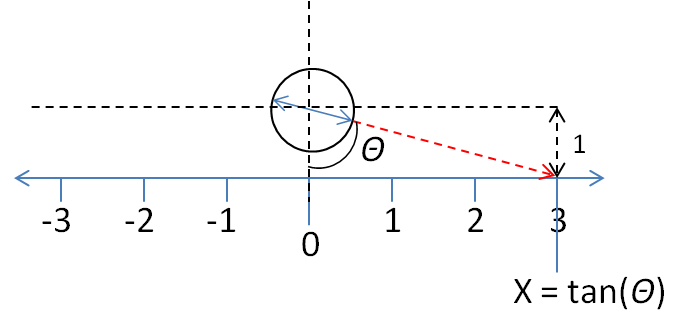
\includegraphics[height=45.1mm,width=102mm]{M2S1 Cauchy Figure.png}
\caption{A spinner 1 unit away from a number line. $\Theta$ is the angle of the spinner, $X$ the number pointed to.}
\end{center}
\end{figure}

\begingroup
\renewcommand*{\arraystretch}{1.5}
$$\begin{array}{rll}
&f_\Theta (\theta) &= \frac{1}{\pi}\\
\Rightarrow \quad &F_\Theta (\theta) &= \int\limits_{-\pi/2}^{\theta}\!\! \frac{1}{\pi} \;\mathrm{d}t\\
& &=\frac{\theta + \pi/2}{\pi}\\
\Rightarrow \quad &F_X(x) &= P(X \leq x)\\
& &= P\left(\tan(\Theta) \leq x \right)\\
& &= P\left(\Theta \leq arctan(x)\right)\\
& &= \frac{1}{\pi}\left(arctan (x) + \frac{\pi}{2}\right)\\
& &= \frac{1}{2} + \frac{1}{\pi} arctan(x)\\
\Rightarrow \quad &f_X(x) &= \frac{\mathrm{d}}{\mathrm{d}x}\left(\frac{1}{2} + \frac{1}{\pi} arctan(x)\right)\\
& &= \frac{1}{\pi} \frac{\mathrm{d}}{\mathrm{d}x}\left( arctan(x)\right)\\
& &= \frac{1}{\pi (1 + x^2)} \quad : \; -\infty < x < +\infty
\end{array}$$

\endgroup
\end{ex}
$\qquad$This distribution for $X$ is called the Cauchy distribution. The ratio of two i.i.d. standard Normal r.v.s is Cauchy (not proved here). We gave a derivation from first principles rather than using the above result for injective transformations purely for illustrative purposes. It is easy to check that the same result will be obtained by either method.

What if we wish to apply a non-injective transformation? The standard technique then is to proceed by considering the c.d.f. This is best shown with an example:

\begin{ex}[Non-Injective Transformations]

$\quad$Suppose $X \sim Uniform(-1, 3)$ s.t. $f_X(x) = 1/4, \; F_X(x) = (x + 1)/4 \; : -1 < x < 3$. Let $Y = X^2$. Find the p.d.f. of $Y$.
\end{ex}

Observe that the transformation function is injective for $x > 1$, so we can simply write $X = \sqrt Y : 1 < Y < 9$. So by the above theorem for injective functions,
\begin{align*}
f_Y(y) &= f_X(\sqrt y) \left| \frac{\mathrm{d}}{\mathrm{d}y}(\sqrt y) \right|\\
&= \frac{1}{8 \sqrt y} \;\; : 1 < y \leq 9
\end{align*}

Now consider $0 \leq y \leq 1$. We cannot apply our result for injective functions, but, by considering the c.d.f., much as we did in example \ref{Cauchy}, we can reach the desired result:
\begin{align*}
F_Y(y) &= P(Y \leq y)\\
&= P(X^2 \leq y)\\
&= P(-\sqrt y \leq X \leq +\sqrt y)\\
&= P(X \leq \sqrt y) - P(X \leq -\sqrt y)\\
&= F_X(\sqrt y) - F_X(- \sqrt y)\\
&= \frac{1}{4}[(\sqrt y + 1) - (-\sqrt y + 1)]\\
&= \frac{\sqrt y}{2}\\
\Rightarrow\quad f_Y(y) &= \frac{1}{4 \sqrt y} \; \; : 0 \leq y \leq 1
\end{align*}\hfill $Q.E.I.$

\noindent Combining these two results:
$$f_Y(y) = \left\{ \begin{array}{ccl} \frac{1}{4 \sqrt y} \;\; &: \;\; &0 \leq y \leq 1\\ \frac{1}{8 \sqrt y} \;\; &: \;\; &1 < y \leq 9 \end{array}\right.$$

\clearpage
\section{Expectation and Higher Moments}$\;$

It is often desirable to pr\'ecis the information in a distribution with a single number or a few numbers. A useful way of doing this is via the \uline{moments} of the r.v.

\subsection{Expectation}$\;$

\begin{defn}[Expectation]
\vspace{1cm}

The first and most commonly used moment is the \uline{expectation}, or mean, which gives us a summary of the location of the probability mass of the distribution. It is defined as follows:\par
\vspace{1cm}
\noindent For $X$ a discrete r.v.:
$$E_{f_X}(X) = \sum_{\mathcal{X}}x f_X(x)$$

\noindent For $X$ a continuous r.v.:
$$E_{f_X}(X) = \int\limits_{\mathcal{X}} x f_X(x)\; \mathrm{d}x$$

\end{defn}

Read ``the expectation of $X$ under the density $f_X$,'' or simply ``under the density of $X$.'' This may seem like an unecessary, tautological notation, but when considering multivariate distributions, it can be very useful to keep track of the subscripts on expectations. Although the notation is standard, it can be unwieldy at times, so the subscripts may be omitted when the meaning is clear; for clarity and legibility, we will tend to write expectations here simply as $E_X(X)$, rather than $E_{f_X}(X)$.

It is also possible to find the expectation of a function of a r.v.:

$$E_{X}(g(X)) = \int\limits_{\mathcal{X}} \!\!g(x) f_X(x)\; dx$$
for continuous $X$ and the analagous sum in the discrete case. In the following we will typically give only the continuous form; this can be converted into the discrete form simply by changing the integral to a summation.

A useful result, not proved here, is that if the expectation of the absolute value of $X$ exists, then so too does the expectation of $X$. This can help in determining the convergence of these integrals/sums.

It is trivial to show from the properties of the integral and of summation that expectation is a linear operator. That is to say:
$$E_{X}(aX + b) = aE_{X}(X) + b$$

It is often useful when calculating the expectation of a r.v. to find a way to transform the integral and then relate the integrand to the p.d.f. of a known distribution over its support - this allows the integral to be evaluated immediately. The following example illustrates this:

\begin{ex}[The Expectation of the Normal Distribution]
\vspace{1cm}

$\quad$Let $X \sim N(\mu, \sigma^2)$, s.t $f_X(x) = 1/\sqrt{2 \pi \sigma^2} exp[-(x - \mu)^2/\sigma^2]$. Find the expectation of $X$.
\end{ex}

\begin{align*}
E_{X}(X) &= \int\limits_{\mathbb{R}}\!\! \frac{x}{\sqrt{2 \pi \sigma^2}} e^{-(x - \mu)^2/2\sigma^2}\;\mathrm{d}x\\
&= \int_{-\infty}^{+\infty}\!\!\frac{y + \mu}{\sqrt{2 \pi \sigma^2}}e^{-y^2/2\sigma^2}\;\mathrm{d}y \; : \; y := x - \mu \\
&= \int_{-\infty}^{+\infty}\!\! \frac{y}{\sqrt{2 \pi \sigma^2}}e^{-y^2/2\sigma^2}\;\mathrm{d}y + \int_{-\infty}^{+\infty} \!\!\frac{\mu}{\sqrt{2 \pi \sigma^2}}e^{-y^2/2\sigma^2}\;\mathrm{d}y \\
&= \mu \int_{-\infty}^{+\infty} \!\!\frac{1}{\sqrt{2 \pi \sigma^2}}e^{-y^2/2\sigma^2}\;\mathrm{d}y\quad \text{ as the other integrand is odd}
\end{align*}

But observe that the integrand is simply the p.d.f. of a Normal r.v.: $Y \sim N(0,\sigma^2)$, hence its integral over the whole real line (the support of $Y$) is 1.
$$\Rightarrow \quad E_{X}(X) = \mu$$
\hfill $Q.E.I.$

\noindent Similarly, in the discrete case:

\begin{ex}[The Expectation of a Binomial R.V.]
\vspace{1cm}

$\quad X \sim Binomial(n, p)$ s.t.$f_X(x) =$ $^nC_x p^x (1 - p)^{n - x}$ Find the expectation of $X$.
\end{ex}

\begin{align*}
E_{X}(X) &= \sum_{x = 0}^n \frac{n!}{x! (n - x)!} x p^x (1 - p)^{n - x}\\
&= \sum_{x = 1}^n \frac{n!}{(x - 1)! (n - x)!} p^x (1 - p)^{n - x}\\
&= np \sum_{x = 1}^n \frac{(n - 1)!}{(x - 1)! (n - x)!}p^{x - 1} (1 - p)^{n - x}\\
&= np \sum_{y = 0}^{n - 1} \frac{(n - 1)!}{y! (n - 1 - y)!} p^y (1 - p)^{n - 1 - y} \; : \; y = x - 1\\
\end{align*}
But the summand is the p.m.f. of $Y \sim Binomial(n - 1, p)$, summed over the support of $Y$, so the sum is equal to unity, leaving
$$E_{X}(X) = np$$
\hfill $Q.E.I.$

\subsubsection{Monte Carlo Integration}

$\quad$It is possible to use expectation to find numerical approximations to integrals via a method called Monte Carlo Integration. Suppose we wish to evaluate
$$\int\limits_{G}\!\!x g(x)\; \mathrm{d}x$$
where $G \subseteq \mathbb{R}$ is the domain of $g(x)$ and $g$ is such that $g(x) \geq 0 \; : \; \forall x \in G$ and $\int\limits_G\!\! g(x)\;\mathrm{d}x = k$

The function $g_X(x) = g(x)/k$ is then a well-defined p.d.f. for some random variable $X$. Take a sample from this distribution: $X_1, \; X_2, \; ... \; X_n \sim g_X(x)$ for some large $n$, $X_i$ i.i.d. Then let $\mu = E_{g_X}(X_i)$. Then, by the linearity of expectation:
$$\overline{X_n} = E_{g_X}(\frac{1}{n}\sum_{i = 1}^n X_i) = \mu$$

\noindent Therefore, $\overline{X_n}$ gives us an estimate for $\mu$. But by the definition of expectation:
$$\mu = \int\limits_G \!\!xg_X(x)\; \mathrm{d}x = \frac{1}{k}\int\limits_G \!\!xg(x)\;\mathrm{d}x$$
So we conclude that $k\overline{X_n}$ is an estimate for the integral we desire to find. More generally, we have:
$$\frac{k}{n} \sum_{i=1}^n f(X_i) \approx \int\limits_G \!\!f(x)g(x)\;\mathrm{d}x$$

This gives us a useful way of estimating integrals where the integrand can be written $f(x)g(x)$, where $g(x) \geq 0$ over the range of integration and $\int g(x)\mathrm{d}x = k$ is a known constant, where the integral is over the same range as the integral we wish to estimate.

In some situations, we might not be able to sample the p.d.f. $g_X(x)$. We can overcome this if we can find another p.d.f., $h_X(x)$, with $G \subseteq \mathcal{X}_h$; i.e., the support of $X$ distributed according to $g_X(x)$ contained in the support of $X$ distributed according to $h_X(x)$. That is simply to say, $h_X(x)$ must be everywhere non-zero where $g$ is non-zero ($h_X$ may, however, be non-zero in places for which $g$ is zero). This requirement enables us to divide by $h_X(x)$ without any problems arising anywhere in the range of integration, $G$. Thus, we write:
$$\int\limits_G \!\!f(x)g(x)\;\mathrm{d}x = \int\limits_G \!\!f(x) \frac{g(x)}{h_X(x)} h_X(x)\; \mathrm{d}x = \int\limits_G\!\! f(x)w(x) h_X(x) \;\mathrm{d}x$$
where $w(x) = g(x)/h_X(x)$ is called an \emph{importance weight}.

We then sample $h_X$: $X_1, \; ... \; X_n \sim h_X(x)$ i.i.d. and approximate the integral as before:
$$\frac{k}{n} \sum_{i = 1}^n w(X_i)f(X_i) \approx \int\limits_G \!f(x) g(x)\; \mathrm{d}x$$
This technique is known as \emph{importance sampling.}

Importance sampling works best when the weights are all roughly equal. This requires the bulk of the probability density of $g_X$ to be entirely within the bulk of $h_X$'s density. Otherwise samples which occur but rarely can have enormous weight, skewing the estimate substantially. Figure \ref{importance sampling} illustrates this. For this reason, it is usually best to choose $h_X$ with ``heavy tails'' or with a support extending far beyond that of $g$ in both directions.

In Figure \ref{importance sampling}, there are three regions of interest noted, A, B and C. In A, values occur fairly frequently (most of the probability mass of $h$, the sampling distribution, is in this region, but the samples here have a very low importance weight, so are suppressed. A moderate number of sample points are likely to occur in B and they will have a reasonable weight attached. In C, although samples are extremely rare, their weights are so high that they will skew the estimate substantially. In this case, then, $h$ would be a very bad sampling distribution to use to obtain a Monte Carlo estimate of the integral.

\begin{figure}[h]
\begin{center}
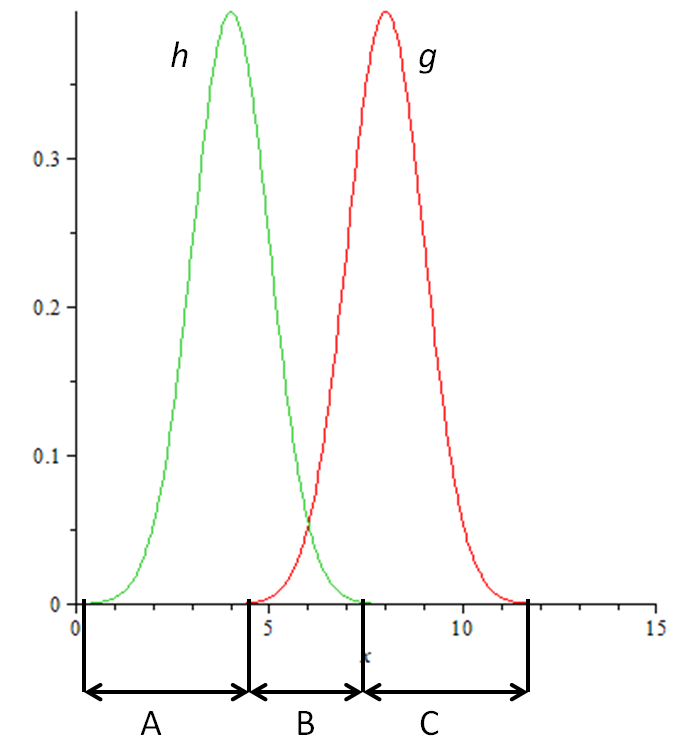
\includegraphics[height=12.6cm,width=11.44cm]{M2S1 Importance Sampling.png}
\caption{density functions of $g$ and $h$, with three regions of note labelled}\label{importance sampling}
\end{center}
\end{figure}

\subsection{Higher Moments}$\;$

Expectation is not the only useful quantity in describing a distribution. In general, the \uline{$\mathrm{k^{th}}$ moment} is defined as the expectation of $X^k$:

\begin{defn}[The $\mathbf{k^{th}}$ Moment]
$$E_{X}(X^k) = \int\limits_{\mathcal{X}}\! x^k f_X(x) \;\mathrm{d}x$$
With an equivalent definition in terms of summation for the discrete case.
It is often more useful to consider the \uline{$\mathrm{k^{th}}$ central moment}, defined as:
$$E_{X}[(X - \mu)^k] = \int\limits_{\mathcal{X}}\! (x - \mu)^k f_X(x)\;\mathrm{d}X$$
where $\mu$ is the expectation (the $\mathrm{1^{st}}$ moment).
\end{defn}

Most useful of these is the \emph{variance}, the $\mathrm{2^{nd}}$ central moment, which gives a measure of the spread of the data. The following result, using the linearity property of expectation, is often extremely useful in evaluating the variance:
\begin{align*}
Var_{X}(X) &= E_{X}[(X - \mu)^2]\\
&= E_{X}(X^2 - 2X\mu + \mu^2)\\
&= E_{X}(X^2) - 2\mu E_{X}(X) + \mu^2\\
&= E_{X}(X^2) - 2\mu^2 + \mu^2\\
&= E_{X}(X^2) - \mu^2
\end{align*}

It is easy to show that variance has the property that:
$$Var_{X}(aX + b) = a^2 Var_{f_X}$$

Because the units of the variance are the square of the units of the variable itself, it is often convenient to consider the \uline{standard deviation} (\uline{s.d.}), which is defined to be the square root of the variance and given the symbol $\sigma$:
$$\sigma = \sqrt{Var_{f_X}(X)}$$
Just as $\mu$ is often used to denote the mean, variance is often denoted $\sigma^2$.

\clearpage
\section{Univariate Distributions}$\;$

In this section, we will look at many of the common, univariate distributions. This should primarily be revision of material covered in M1S. Three new continuous distributions (Beta, chi-squared and Student's-t) will be introduced, but without detailed analysis; we will simply assert the results. They will see some use later in the course.

\subsection{Discrete Distributions}

\subsubsection{The Discrete Uniform Distribution: $X \sim DiscreteUnif(n)$}

$\quad$An extremely simple distribution, this models simple situations such as rolling a die, with a finite number of equiprobable outcomes. The probability mass and cumulative distribution functions are:
\begin{align*}
f_X(x) &= \frac{1}{n} \; : x = x_1, \; x_2, \; ... x_n\\
F_X(x) &= \frac{\lfloor x \rfloor}{n} \; \mbox{where $\lfloor x \rfloor$ here denotes the largest $x_i \leq x$}
\end{align*}

\subsubsection{The Bernoulli Distribution: $X \sim Bernoulli(\theta)$}

$\quad$Another almost trivial distribution, but this one is useful for building up larger distributions. A Bernoulli distribution has a single event with two possible outcomes (often referred to as ``success'' and ``failure'') with known probabilities. In fact, a Bernoulli trial may have more than two outcomes, so long as we are only interested in two mutually exclusive and exhaustive \emph{events}; for instance, if we roll a (normal) die, there are six possible outcomes, but if we are only interested in whether or not we roll a six, then we may group the other five outcomes together as a single event and model the roll as a Bernoulli trial.

Letting $X=1$ denote ``success'' and $X=0$ ``failure,'' the distribution functions and first two (central) moments for a Bernoulli r.v. are:
\begin{align*}
f_X(x) &= \left\{ \begin{array}{cl} \theta \quad & : \; x = 1\\ 1-\theta \quad & : \; x = 0 \end{array} \right. = \theta^x(1-\theta)^{1-x} \; : x \in \mathcal{X}\\
F_X(x) &= \left\{ \begin{array}{cl} 0 \quad & : \; x < 0\\ 1-\theta \quad & : \; 0 \leq x < 1\\ 1 \quad & : \; x \geq 1 \end{array} \right.\\
E_{X}(X) &= \theta\\
Var_{X}(X) &= \theta(1-\theta)\\
\mathcal{X} &= \{0,1\}
\end{align*}

\subsubsection{The Binomial Distribution: $X \sim Binomial(n,\theta)$}

$\quad$Suppose $X_i \sim Bernoulli(\theta) \; : i = 1,\; 2,\; ... n$ are $n$ i.i.d. Bernoulli r.v.s with probability $\theta$. Define $X = \sum_{i=1}^n X_i$. Then $X \sim Binomial(n, \theta)$ is a binomial r.v. with $n$ trials and probability $\theta$. That is to say that a binomial r.v. records the number of ``successes'' in $n$ independent, identically distributed Bernoulli trials.

It is easy to derive the p.m.f., c.d.f., mean and variance of a binomial r.v. from the Bernoulli distribution. They are:
\begin{align*}
f_X(x) &= \frac{n!}{x! (n - x)!} \theta^x (1 - \theta)^{n - x}\\
F_X(x) &= \left\{ \begin{array}{cl} 0 \quad & : \; x < 0\\ \sum\limits_{i=0}^{x} \frac{n!}{i! (n - i)!} \theta^i (1 - \theta)^{n - i} \quad & : \; 0 \leq x < n\\ 1 \quad & : \; x \geq n \end{array} \right.\\
E_{X}(X) &= n\theta\\
Var_{X} &= n\theta(1-\theta)\\
\mathcal{X} &= \{1,\; 2,\; ... \; n\}
\end{align*}

The c.d.f. does not have an elegant closed form, so it is usual to consider and write only the p.m.f. This practice will hereafter be followed and c.d.f.s only given when they have a simple form.

\subsubsection{The Geometric Distribution: $X \sim Geo(\theta)$}

$\quad$Consider a sequence of repeated, i.i.d. Bernoulli trials with parameter $\theta$, as for the binomial distribution, except proceeding without limit, rather than having a fixed number of trials. Let $X$ be the number of trials before the first success (including the trial on which that success occurs). Then $X \sim Geo(\theta)$. Clearly, $P(X=x)$ is the probability of having $x-1$ failures followed by 1 success, so for a geometric r.v.:
\begin{align*}
f_X(x) &= \theta (1-\theta)^{x-1}\\
F_{X}(x) &= 1 - (1-\theta)^x\\
E_{X}(X) &= \frac{1}{\theta}\\
Var_{X} &= \frac{1-\theta}{\theta^2}\\
\mathcal{X} &= \mathbb{Z}^+
\end{align*}

\subsubsection{The Negative Binomial Distribution: $ X \sim NegBin(n,\theta)$}

$\quad$Similar to the geometric distribution, consider an infinite sequence of i.i.d. Bernoulli trials, except that this time $X$ denotes the number of trials up to and including the $n^{th}$ success. Sometimes it is convenient to subtract $n$ from this, so that $X$ represents the number of trials \emph{after the $n^{th}$} trial before the $n^{th}$ success/ This gives rise to two alternative forms for the p.m.f., range, mean and variance:
\begin{align*}
f_X(x) &= \left(\!\!\!\begin{array}{c} x-1 \\ n-1 \end{array}\!\!\!\right) \theta^n (1-\theta)^{x-n}\\
E_{X}(X) &= \frac{n}{\theta}\\
Var_{X}(X) &= \frac{n(1-\theta)}{\theta^2}\\
\mathcal{X} &= \mathbb{Z}_{\geq n}
\end{align*}

\begin{center} or \end{center}
\begin{align*}
f_X(x) &= \left(\!\!\!\begin{array}{c} n+x-1 \\ x \end{array}\!\!\!\right) \theta^n (1-\theta)^x\\
E_{X}(X) &= \frac{n(1-\theta)}{\theta}\\
Var _{X}(X) &= \frac{n(1-\theta)}{\theta^2}\\
\mathcal{X} &= \mathbb{Z}_{\geq 0}
\end{align*}
In the above, we use bracket notation for combinations, so that:
$$\left(\!\!\!\begin{array}{c} n\\x\end{array}\!\!\!\right) = \frac{n!}{x! (n-x)!}$$

\subsubsection{The Hypergeometric Distribution: $X \sim Hypergeo(N,R,n)$}

$\quad$Consider a population of $N$ objects/people/\&c., of which $R$ are of ``type I'' and the remaining $N-R$ of ``type II.'' Suppose we take a random sample of size $n$ and let $X$ be the number of type I's in the sample. By combinatorial reasoning, considering the number of ways of choosing the sample, it is clear that:
\begin{align*}
f_X(x) &= \frac{\left(\!\!\! \begin{array}{c} R\\ x\end{array}\!\!\!\right) \left(\!\!\!\begin{array}{c} N-R\\ n-x \end{array}\!\!\!\right)}{\left(\!\!\!\begin{array}{c} N\\ n\end{array}\!\!\!\right)}\\
\mathcal{X} &= [max\{0,n-(N-R)\},min\{n,r\}]
\end{align*}
We also find:
\begin{align*}
E_{X}(X) &= \frac{n(N-R)}{N}\\
Var_{X}(X) &= \frac{nR(N-R)(N-n)}{N^2(N-1)}
\end{align*}
These last two results are included for completeness only and were not covered in the course.

\subsubsection{The Poisson Distribution: $X \sim Poisson(\lambda)$}

$\quad$Suppose we have $n$ i.i.d. Bernoulli trials, as for the binomial distribution. But now suppose $\theta = \lambda/n$ for some constant $\lambda$. Now let $n \rightarrow \infty$, $\theta \rightarrow 0$ and observe:
\begin{align*}
\lim_{n \rightarrow \infty} \left[\frac{n!}{x! (n - x)!} \theta^x (1 - \theta)^{n - x}\right] &= \frac{1}{x!}\lim_{n \rightarrow \infty} \left[\frac{\lambda^x}{n^x} \frac{n!}{(n-x)!} (1-\theta)^{n-x}\right]\\
&= \frac{\lambda^x}{x!}\lim_{n\rightarrow\infty}\left[ \frac{n!}{n^x (n-x)!}\left(1 - \frac{\lambda}{n}\right)^{n-x}\right]\\
&= \frac{e^{-\lambda}\lambda^x}{x!}\lim_{n\rightarrow\infty} \left[\frac{n!}{n^x(n-x)!}\right]
\end{align*}
where we have used, with $a = -\lambda$, the fact that:
$$\lim_{n\rightarrow\infty}\left[\left(1+\frac{a}{n}\right)^{n}\right] = e^a$$

Now, observe that:
\begin{align*}
\frac{n!}{n^x(n-x)!} &= \frac{\prod\limits_{i=1}^n\!\! i}{\prod\limits_{i=1}^x\!\! n \times \prod\limits_{i=1}^{n-x} \!\!i}\\
&= \frac{\prod\limits_{i=n-x+1}^n\!\! i}{\prod\limits_{i=n-x+1}^n \!\!n}\\
&= \prod\limits_{i=n-x+1}^n \!\!\frac{i}{n}\\
&= \frac{n-x+1}{n}\times\frac{n-x+2}{n}\times\; ... \; \times \frac{n-1}{n} \times \frac{n}{n}\\
&= \left(1 - \frac{x-1}{n}\right) \times \left(1 - \frac{x-2}{n}\right)\times \; ...\; \times \left(1 - \frac{1}{n}\right) \times 1\\
&\rightarrow 1 \text{ as } n \rightarrow \infty
\end{align*}

Hence we conclude that for a binomial r.v. $X$, if $p = \lambda/n$:
$$f_X(x) \rightarrow \frac{e^{-\lambda}\lambda^x}{x!} \text{ as } n \rightarrow \infty$$

We define a Poisson r.v. to be one following this distribution. We can regard this as a sequence of Bernoulli events occurring in a time $T$, divided into $n$ subintervals of length $T/n$. If events in separate subintervals are independent of one another, as $n \rightarrow \infty$, there will be at most 1 event in each subinterval and the probability of an event occurring in a given subinterval will be the same for all intervals, proportional to the length $T/n$ of the interval. Let $X$ be the number of events occurring in time $T=1$. Then as $n \rightarrow \infty$, the limiting distribution of $X$ is Poisson.

This distribution is often useful for modelling events which occur at a certain, fixed rate, independently of one another. Radioactive decay is very successfully modelled as a Poisson r.v., for example. For $X \sim Poisson(\lambda)$:
\begin{align*}
f_X(x) &= \frac{e^{-\lambda}\lambda^x}{x!}\\
E_{X}(X) &= \lambda\\
Var_{X}(X) &= \lambda\\
\mathcal{X} &= \mathbb{Z}_{\geq 0}
\end{align*}

The Poisson process described above also leads to some continuous probability distributions.

\subsection{Continuous Distributions}

\subsubsection{The Exponential Distribution: $X \sim Exp(\lambda)$}

$\quad$Consider a Poisson process, as in the previous section. Let $X$ be the time until the first event (or, equivalently, between the $n^{th}$ and $(n+1)^{th}$ events). Then\\ $P(X>x) = P(\{\text{no events in the interval of length $y$}\})$. Hence:
\begin{align*}
 P(Y>y) &= \frac{e^{-\lambda y}(\lambda y)^0}{0!}\\
 &= e^{-\lambda y}\\
\Rightarrow \quad F_Y(y) &= 1 - e^{-\lambda y}\\
\Rightarrow\quad f_X(x) &= \lambda e^{-\lambda y}
\end{align*}

This is the p.d.f. of an exponential r.v. Its c.d.f., as found in the derivation above, is $1-e^{-\lambda x}$. Its mean and variance are:
$$E_{X}(X) = \frac{1}{\lambda}$$
$$Var_{X}(X) = \frac{1}{\lambda^2}$$

The exponential distribution exhibits an interesting and useful property called \uline{lack of memory}. It is the only continuous distribution with this property.

\begin{prop}[The Lack of Memory Property]$\quad$\par
\vspace{1cm}

For $X \sim Exp(\lambda)$, $P(X>x\; | \; X>x_0) = P(X>x-x_0)$
\end{prop}

\noindent\textsc{Proof:}
\begin{align*}
P(X>x\; | \; X>x_0) &= P(X > x_0 + a\; | \; X > x_0) \; : \; a>0\\
&= \frac{P(\{X > x_0 + a\}\cap \{X > x_0\})}{P(X > x_0)}\\
&= \frac{P(X > x_0 + a)}{P(X > x_0)}\\
&=\frac{e^{-\lambda (x_0 + a)}}{e^{-\lambda x_0}}\\
&= e^{-\lambda a}\\
&= e^{-\lambda (x-x_0)}\\
&= P(X>x-x_0)
\end{align*}
\hfill$Q.E.D.$

\subsubsection{The Gamma Distribution: $X \sim \Gamma(\alpha,\beta)$}

Before considering this distribution, we require a new function:

\begin{defn}[The Gamma Function]
$$\Gamma(x) = \int_0^{\infty}\!\!t^{x-1}e^{-t}\;\mathrm{d}t \; : \; x>0$$
\end{defn}

\noindent The Gamma function has several useful properties:

\begin{prop}[Properties of the Gamma function]$\quad$\par
\textbf{1:}  $\Gamma(x) = (x-1)\Gamma(x-1)$\par
\textbf{2:} $\Gamma(1) = 1$\par
\textbf{3:} $\Gamma(n) = (n-1)! \; : \; n \in \mathbb{N}$\par
\textbf{4:} $\Gamma(1/2) = \sqrt \pi$\par
\end{prop}

\noindent\textsc{Proof:}\par
\textbf{1:}
\begin{align*}
\Gamma(x) &= \int_0^\infty \!\! t^{x-1}e^{-t}\;\mathrm{d}t\\
&=\left[ -t^{x-1}e^{-t}\right]_0^\infty + (x-1)\int_0^\infty\!\! t^{x-2}e^{-tx}\;\mathrm{d}t\\
&= (x-1)\Gamma(x-1)
\end{align*}
\hfill$Q.E.D.$

\noindent \textbf{2:}
\begin{align*}
\Gamma(1) &= \int_0^\infty \!\! e^{-t}\;\mathrm{d}t\\
&= \left[-e^{-t}\right]_0^\infty\\
&= 1
\end{align*}
\hfill$Q.E.D.$

\noindent \textbf{3:}
\begin{center}
by \textbf{2}, $\Gamma(1) = 1 = 0!$, so true for $n=1$\\
by \textbf{1}, $\Gamma(n+1) = n\Gamma(n)$\\
hence if $\Gamma(n)=(n-1)!$, then $\Gamma(n+1) = n!$\\
hence, by induction, $\Gamma(n) = (n-1)! \;\; \forall n \in \mathbb{N}$
\end{center}
\hfill$Q.E.D.$

\noindent \textbf{4:}\par
\indent Proof beyond the scope of this course. The result may be assumed.
\hfill $\blacksquare$\par
\vspace{1cm}

Let $X$ be the waiting time for the $r^{th}$ event in a Poisson process. In order to help us derive the distribution for $X$, we define $Y$ to be the number of events before time $x$, so that $Y \sim Poisson(\lambda x)$. Then:
\begin{align*}
F_X(x) &= P(X\leq x)\\
&= 1 - P(X > x)\\
&= 1 - P(Y < r)\\
&= 1 - \sum_{y=0}^{r-1} \frac{e^{-\lambda x} (\lambda x)^y}{y!}\\
\Rightarrow \quad f_X(x) &= -\sum_{y=0}^{r-1}\left[\frac{-\lambda e^{-\lambda x} (\lambda x)^y}{y!} + \frac{y\lambda e^{-\lambda x}(\lambda x)^{y-1}}{y!}\right]\\
&= \sum_{y=0}^{r-1}\frac{\lambda e^{-\lambda x}(\lambda x)^y}{y!} - \sum_{y=0}^{r-2} \frac{\lambda e^{-\lambda x}(\lambda x)^y}{y!}\\
&= \frac{\lambda e^{-\lambda x}(\lambda x)^{r-1}}{(r-1)!}\\
&= \frac{\lambda^r}{(r-1)!}x^{r-1}e^{-\lambda x}
\end{align*}

We say $X \sim \Gamma(r-1,\lambda)$. Note that $(r-1)! = \Gamma(r)$. Generally, the p.d.f. of a Gamma r.v. $X$ with parameters $\alpha$ and $\beta$ is given by:
$$f_X(x) = \frac{\beta^\alpha}{\Gamma(\alpha)}x^{\alpha-1}e^{-\beta x}$$

Note that there are two conventions with regards to the parameterisation of the Gamma distribution. Sometimes, the p.d.f. of $X \sim \Gamma(\alpha,\beta)$ is given as:
$$f_X(x) = \frac{1}{\Gamma(\alpha)\beta^\alpha}x^{\alpha -1}e^{-x/\beta}$$

For this reason, it is always important to give the p.d.f. explicitly when discussing a Gamma r.v. The parametrisation used on the formula sheet provided with the course is the first one given above, with $\beta$ in the numerator. Using this parameterisation, the mean and variance of the distribution are:
$$E_{X}(X) = \frac{\alpha}{\beta}$$
$$Var_{X}(X) = \frac{\alpha}{\beta^2}$$

\noindent Based on the above derivation, we see that for $Y_i \sim Poisson(\lambda)$ i.i.d.:
$$\sum_{i=1}^n Y_i \sim Gamma(n,\lambda)$$

\subsubsection{The Continuous Uniform Distribution: $X \sim Unif(\alpha,\beta)$}

$\quad$A trivial distribution, for a r.v. with equal probability density between two endpoints, $\alpha$ and $\beta$. The \uline{standard uniform distribution} has $\alpha = 0$, $\beta = 1$.

$$f_X(x) = \frac{1}{\beta-\alpha}$$
$$F_X(x) = \frac{x-\alpha}{\beta-\alpha}$$
$$E_{X}(X) = \frac{\alpha+\beta}{2}$$
$$Var_{X}(X) = \frac{(\beta-\alpha)^2}{12}$$

\subsubsection{The Normal or Gaussian Distribution: $X \sim N(\mu, \sigma^2)$}

$\quad$An extremely useful distribution, this models all sorts of naturally occurring variables, such as heights or weights of men or women, size of pebbles on a stony beach, \&c. The normal distribution has its mean and variance as its parameters, which is convenient.
\begin{align*}
f_X(x) &= \frac{1}{\sqrt{2\pi\sigma^2}}e^{\frac{-(x-\mu)^2}{2\sigma^2}}\\
E_{X}(X) &= \mu\\
Var_{X}(X) &= \sigma^2\\
\mathcal{X} &= \mathbb{R}
\end{align*}

Of particular interest is the \uline{standard normal distribution}, with mean 0 and variance 1. This distribution is of such importance that it has its own notation; standard normal r.v.s are conventionally denoted $Z$ and the p.d.f. and c.d.f. of the standard normal distribution are denoted $\phi(z)$ and $\Phi(z)$ respectively. $Z \sim N(0,1)$:
$$f_Z(z) = \phi(z) = \frac{1}{\sqrt{2\pi}}e^{-x^2/2}$$
$$F_Z(z) = \Phi(z) = \int_{-\infty}^{z} \!\phi(t)\; \mathrm{d}t$$

The c.d.f., $\Phi(z)$, is not available in closed form, but is calculable to arbitrary accuracy by numerical methods.

It is useful to remember the ``68 - 95 - 99'' rule: the probability of a normal r.v. taking a value within 1, 2 or 3 standard deviations respectively of the mean is roughly 68\%, 95\%, 99\% respectively:
$$P\left( \frac{|X-\mu|}{\sigma}< 1\right) \approx 68\%$$
$$P\left( \frac{|X-\mu|}{\sigma} < 2\right) \approx 95\%$$
$$P\left( \frac{|X-\mu|}{\sigma} < 3\right) \approx 99\%$$

It is sometimes convenient to remember that, more precisely, the probability of a normal r.v. taking a value within $1.96\sigma$ of the mean is 95\%

\subsubsection{The Normal Approximation to the Binomial Distribution}\label{normal approx to bin}

$\quad$The Central Limit Theorem (to be covered later) allows us to approximate many distributions as Normal for appropriate values of their parameters. We will illustrate this for a binomial r.v., $X \sim Binomial(n,\theta)$. $E_{f_X}(X) = n\theta$ and $Var_{f_X}(X) = n\theta(1-\theta)$. Then:
$$X \sim_{approx} N(n\theta,n\theta(1-\theta))$$
for large $n$. As a general rule-of-thumb, the Normal approximation of a binomial r.v. is useful for\\$min\{n\theta,n\theta(1-\theta)\} \geq 10$.

\begin{ex}
\vspace{1cm}

Suppose $X \sim Binomial(100,0.1)$. Then $\mu = 10$, $\sigma^2 = 9$:
\begin{align*}
P(X \leq 9) &\approx P\left(Z \leq \frac{9-10}{3}\right)\\
&=P\left(Z \leq \frac{-1}{3}\right)\\
&= \Phi\left(\frac{-1}{3}\right)\\
&= 1-\Phi\left(\frac{1}{3}\right)\\
&\approx 37.07\%
\end{align*}
\end{ex}

The exact answer can be calculated from the binomial distribution as roughly 45.13\%. Here, the Normal approximation is fairly poor. We can improve it with the \uline{continuity correction}. Figure \ref{normal approximation} illustrates the reason for the error.

\begin{figure}[h]
\begin{center}
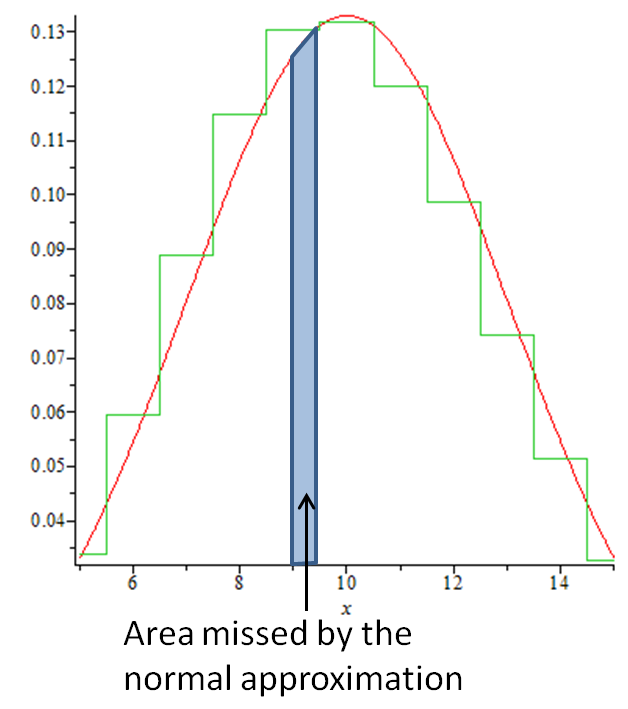
\includegraphics[height=11.97cm,width=10.6cm]{M2S1 Normal Approximation.png}
\caption{The Normal approximation to a Binomial r.v., illustrating the area missed, requiring the continuity correction}\label{importance sampling}\label{normal approximation}
\end{center}
\end{figure}

As the binomial distribution is discrete, $P(X \leq 9) = P(X \leq 9.5)$. We find that, using the Normal approximation, this gives us a much better estimate, of 43.25\%, which is close to the correct answer of 45.13\%. Thus, when using a continuous distribution to approximate a discrete r.v., we set $P(X \leq x) = P(X \leq x+0.5)$ and $P(X < x) = P(X \leq x-0.5)$. Great care must be taken with the strictness (or not) of inequalities.

\subsubsection{The Beta Distribution: $X \sim Beta(\alpha,\beta)$}

$\quad$The Beta distribution has support $(0,1)$, making it extremely useful for representing probabilities. This will be examined in more depth later in the course. For now, we merely cite the following results:
\begin{align*}
f_X(x) &= \frac{\Gamma(\alpha + \beta)}{\Gamma(\alpha)\Gamma(\beta)}x^{\alpha-1}(1-x)^{\beta-1}\\
E_{X}(X) &= \frac{\alpha}{\alpha + \beta}\\
Var_{X}(X) &= \frac{\alpha\beta}{(\alpha + \beta)^2(\alpha + \beta + 1)}\\
\mathcal{X} &= (0,1)
\end{align*}

\subsubsection{The Chi-Squared Distribution: $X \sim \chi^2_n$}

$\quad$Conventionally, the parameter for the $\chi^2$ distribution, $n$, called the \uline{degrees of freedom} of the r.v., is denoted by a subscript rather than in parentheses, as with most distributions.

Suppose $Z \sim N(0,1)$. Let $X = Z^2$. Then $X \sim Gamma(1\!/\!2,1\!/\!2) \sim \chi^2_1$. The chi-squared distribution is actually a special case of the Gamma distribution. More generally, if $Z_i \sim N(0,1)$ i.i.d., $X = \sum\limits_{i=1}^n Z_i^2$, then $X \sim Gamma(n\!/\!2,1\!/\!2) \sim \chi^2_n$
\begin{align*}
f_X(x) &= \frac{1}{2^{\frac{n}{2}}\Gamma\left(\frac{n}{2}\right)} x^{\frac{n}{2}-1}e^{-\frac{x}{2}}\\
E_{X}(X) &= n\\
Var_{X}(X) &= 2n\\
\mathcal{X} &= \mathbb{R}^+
\end{align*}

\subsubsection{Student's t-Distribution: $ X \sim t_n$}

$\quad$Again, as with the chi-squared distribution, the degrees of freedom of the distribution are denoted with a subscript, rather than in parentheses. Let $Z \sim N(0,1)$, $Y \sim \chi^2_n$. Let $X = Z/\sqrt{Y/}$. Then $X \sim t_n$ $t_1$ is the Cauchy distribution seen in example \ref{Cauchy}.
\begin{align*}
E_{X}(X) &= \left\{ \begin{array}{cl} 0 \quad& : \; n > 1\\ \mbox{undefined}\quad& : \; \mbox{otherwise}\end{array}\right.\\
Var_{X}(X) &= \left\{\begin{array}{cl} \frac{n}{n-2} \quad& : \; n>2\\ \mbox{undefined}\quad& \mbox{otherwise}\end{array}\right.\\
F_X(x) &\rightarrow \Phi(x) \;\; \text{as }\; n\rightarrow \infty
\end{align*}

\subsection{Families of Distributions}$\;$

Some distributions form ``families,'' which can be usefully considered together.

\subsubsection{The Exponential Family}

A family of p.d.f.s (or p.m.f.s) is called an exponential family if
$$f_X(x\; | \; \vec{\theta}) = h(x) c(\vec{\theta}) e^{\sum\limits_{i=1}^k w_i(\vec{\theta}) t_i(x)}$$
where $\vec{\theta}$ is a vector of parameters.

We call $w_1(\vec{\theta}),\; w_2(\vec{\theta}),\; ...\; w_k(\vec{\theta})$ the \uline{canonical parameterisation} or \uline{natural parameterisation}.

\begin{ex}[The Gamma Distribution]
\vspace{1cm}

Let $X \sim \Gamma(\alpha, \beta)$. Then:
\begin{align*}
f_X(x) &= \frac{1}{\Gamma(\alpha) \beta^\alpha} x^{\alpha-1}e^{-x/\beta}\\
&= \frac{1}{\Gamma(\alpha)\beta^\alpha}e^{(\alpha-1)log(x) - \frac{1}{\beta}x}
\end{align*}

Let $\vec{\theta} = (\alpha,\beta)$, $h(x) = 1$, $c(\alpha,\beta) = 1/(\Gamma(\alpha)\beta^\alpha)$, $w_1(\alpha,\beta) = (\alpha-1)$, $t_1(x) = log(x)$,\\ $w_2(\alpha, \beta) = 1/\beta$ and $t_2(x) = -x$. Then we see that the Gamma distribution is a member of the exponential family and has canonical parameterisation $(\alpha-1),\; 1/\beta$.

\end{ex}

\begin{ex}[A Cautionary Non-Example]
\vspace{1cm}

Let $f_X(x) = 1/\theta e^{1-x/\theta}\; : \; 0<\theta<x$. Then $f_X(x)$ is \textbf{not} a member of the exponential family, because although the p.d.f. has an appropriate form, the support is in terms of the parameter $\theta$; because of this, we can define an 'indicator function':
$$I\{\theta<x\} = \left\{\begin{array}{cl} 0 \quad :& \theta \geq x\\ 1\quad :& \theta<x \end{array}\right.$$
and then write:
$$f_X(x) = \frac{e}{\theta}e^{-\frac{1}{\theta}x}I\{\theta < x\}\; : \; x>0$$
And, though the first part is in the form for a member of the exponential family, the indicator function cannot be split into functions purely in $x$ and purely in $\theta$.

\end{ex}

\subsubsection{Location-Scale Families}

$\quad$Let $Z$ be a r.v. distributed according to $f_Z(z)$. Let $X_1 = Z+\mu$ for some constant $\mu$. Then $X_1$ is a member of the same \uline{location family} as $Z$. Now let $X_2 = \sigma Z$ for some constant $\sigma$. Then $X_2$ is in a \uline{scale family} with $Z$. Finally, let $X = \sigma Z + \mu$; then $X$ is in a \uline{location-scale family} with $Z$. $\mu$ is called a \uline{location parameter}, $\sigma$ a \uline{scale parameter}.

It is no co\"incidence that we used $\mu$ and $\sigma$ for the constants; it is often convenient to relate a r.v. to the one obtained by subtracting the mean and then dividing by the standard deviation. This is typically some sort of standard version of the distribution. By the properties of expectation and variance proved earlier, if $E(Z) = 0$ and $Var(Z) = 1$, then for $X=\sigma Z + \mu$, $E(X) = \mu$ and $Var(X) = \sigma^2$. Even more importantly:
$$P(a<X<b) = P\left(\frac{a-\mu}{\sigma}<Z<\frac{b-\mu}{\sigma}\right)$$

This means that if we can evaluate probabilities for $Z$, we can evaluate them for any $X$ in a location-scale family with $Z$. This lets us create standard tables of probability that are still widely applicable. For instance, the Normal cumulative distribution function has tabulated values for a range of arguments; from this, any probability associated with any other Normal r.v. can be easily calculated.

\clearpage
\section{Multivariate Random Variables}

\subsection{Introduction}$\;$

In this section, we will study how to model two (or more) r.v.s together with a single, multidimensional distribution. This will give us new tools for considering independence and the relationship between dependent variables. We will focus on bivariate distributions, but the ideas generalise easily to larger numbers of r.v.s.

\begin{defn}[Joint Distribution Functions]
\vspace{1cm}

Let $X$ and $Y$ be discrete r.v.s. Then the \uline{joint mass function} of $X$ and $Y$ is:
$$f_{X,Y}(x,y) = P(X=x \text{ and } Y=y) = P\{s \in S \; | \; X(s) = x \text{ and } Y(s) = y\}$$

Now let $X$ and $Y$ be continuous r.v.s. Then the \uline{joint density function} is any surface $f_{X,Y}(x,y)$ with the property that:
$$P\{s \in S \; | \; (X(s),Y(s)) \in R\} = \iint\limits_R \! f_{X,Y}(x,y)\; \mathrm{d}R$$
for any measurable region $R$.\par
\vspace{1cm}

This definition can trivially be extended to the joint distribution functions of three or more variables. We also define the joint cumulative distribution function:
\begin{align*}
F_{X,Y}(x,y) &= P(X\leq x \text{ and } Y\leq y)\\
&= \left\{ \begin{array}{cl} \int\limits_{-\infty}^y\int\limits_{-\infty}^x\!\! f_{X,Y}(s,t)\;\mathrm{d}s\mathrm{d}t\quad & : \; \text{continuous case}\\ \sum\limits_{t=0}^y\sum\limits_{s=0}^x f_{X,Y}(s,t)\quad & : \; \text{discrete case} \end{array} \right.
\end{align*}

\end{defn}

\subsubsection{Moments of Multivariate Distributions}

$\quad$We can define the expectation of functions of multivariate distributions in the obvious way, generalising from the univariate case:
$$E_{X,Y}(g(X,Y)) = \iint\limits_{\mathcal{X}\times\mathcal{Y}}\!\! g(x,y)f_{X,Y}(x,y)\; \diff x\diff y$$
where the integrals are replaced with summations in the discrete case.

\subsubsection{Marginal Distributions}

$\quad$Given $f_{X,Y}(x,y)$, we can find $f_X(x)$ and $f_Y(y)$; these are called the \uline{marginal distributions} of $X$ and $Y$. Consider first an example in the discrete case:

\begin{ex}[Sex and Age of U.S. College Students]
\vspace{1cm}

The following table summarises the sex- and age-distribution of college students in the U.S.A. in 1985:

\begin{center}
$$\begin{array}{|c|c|c|c|c|c|} \hline
\quad & \textbf{14 - 17} \; & \textbf{18 - 24} \; & \textbf{25-34} \; & \textbf{35+}\; & \mbox{\textbf{Any age}}\\ \hline
\text{\textbf{Male}}\; & 0.01\; & 0.3\; & 0.12\; & 0.04\; & \mathbf{0.47} \\ \hline
\mbox{\textbf{Female}}\; & 0.01\; & 0.3\; & 0.13\; & 0.09 & \mathbf{0.53}\\ \hline
\mbox{\textbf{Either sex}}\; & \mathbf{0.02}\; & \mathbf{0.6}\; & \mathbf{0.25} \; & \mathbf{0.13}\; & \mathbf{1}\\ \hline
\end{array}$$
\end{center}

\end{ex}
$\quad$In the margins of the table, the sums of each row and column have been included. These margins represent the marginal distributions of sex (in the final column) and age (in the bottom row), hence the term ``marginal distribution.'' By the theorem of total probability (see section \ref{total prob}), we know that:
$$P(female) = \sum\limits_i [P(\{female\} \cap \{age = i\})]$$
and similarly for the prior probability of being male. Furthermore,
$$P(age = i) = P(age = i \text{ and } male) +P(age = i \text{ and } female)$$
Thus, by summing along a row or down a column, we find the prior probability of a given sex or age respectively. This leads to the following:

\begin{thm}[Marginal Distributions]$\quad$\par
\vspace{1cm}

$\quad$For $X$, $Y$ discrete r.v.s with joint mass function $f_{X,Y}(x,y)$, the marginal distributions of $X$ and $Y$ are given by:
$$f_X(x) = \sum\limits_{\mathcal{Y}} f_{X,Y}(x,y) \qquad\qquad f_Y(y) = \sum\limits_{\mathcal{X}} f_{X,Y}(x,y)$$

For $X$ and $Y$ continuous r.v.s with joint density function $f_{X,Y}(x,y)$, the marginal distributions are:
$$f_X(x) = \int\limits_{\mathcal{Y}}\!\! f_{X,Y}(x,y)\; \diff y \qquad\qquad f_Y(y) = \int\limits_{\mathcal{X}} \!\! f_{X,Y}(x,y)\; \diff x$$

\end{thm}

\noindent\textsc{Proof:}\\
\indent Trivial, based on the above discussion, so not included here. Simply show that the function given satsifies the properties with respect to probability required of a mass/density function.

Note that it is possible to have $X$ discrete and $Y$ continuous, say. In this case, if we wish to find the marginal of $X$, we would integrate over $\mathcal{Y}$, or, to find the marginal distribution of $Y$, we would sum over $\mathcal{X}$. Whether summing or integrating is determined by the nature of the r.v. over whose support we are perfoming the summation or integration.

\subsection{Independence and Conditional Distributions}$\;$

Recall the conditional probability operator: $P(A|B) = P(A \cap B)/P(B)$. As the joint mass function of a dis\-crete, bi\-vari\-ate r.v. is sim\-ply a prob\-a\-bil\-ity, we can de\-fine the \uline{conditional p.m.f. of $X$ given $Y$} as:
\begin{align*}
f_{X|Y}(x|y) &= P(X = x\; | \; Y = y)\\
&= \frac{P(X = x \text{ and } Y = y)}{P(Y = y)}\\
&= \frac{f_{X,Y}(x,y)}{f_Y(y)}
\end{align*}

Note that this follows simply from previous knowledge. However, to extend this to the continuous case, we must \textbf{define} the conditional density function - density functions are \textbf{not} themselves probabilities and so we cannot directly apply the definition of conditional probability as we did in the discrete case. So we define the conditional probability density function of $X$ given $Y$ to be:
$$f_{X|Y}(x|y) = \frac{f_{X,Y}(x,y)}{f_Y(y)}$$
as above. Now we must justify that this is a useful and meaningful definition. Consider:
\begin{align*}
P(Y\leq y\; | \; X=x) &= \lim_{h\rightarrow 0} [P(Y\leq y\; | \; x\leq X\leq x+h)]\\
&= \lim_{h\rightarrow 0} \left[\frac{P(Y\leq y \text{ and } x\leq X \leq +h)}{P(x\leq X \leq X+h)}\right]\\
&= \lim_{h\rightarrow 0} \left[\frac{\int\limits_x^{x+h}\!\!\int\limits_{-\infty}^y\!\! f_{X,Y}(s,t)\;\diff t\diff s}{\int\limits_x^{x+h}\!\! f_X(s)\;\diff s}\right]
\end{align*}
Note that:
$$\frac{\diff}{\diff h}\!\left(\int_x^{x+h}\!\!\!\!f_X(s)\;\diff s\right) = \frac{\diff}{\diff h}\!\left[F_X(x+h)-F_X(x)\right] = f_X\!(x+h)$$
Also note that the numerator and denominator of the fraction in the above limit tend to 0 and the derivative of the denominator is non-zero in an interval around $x$, so by de l'H\^opital's rule:
\begin{align*}
P(Y\leq y\; | \; X=x) &= \lim_{h\rightarrow 0}\left[\frac{\int\limits_{-\infty}^y\!\! f_{X,Y}(x+h,t)\;\diff t}{f_X(x+h)}\right]\\
&= \int_{-\infty}^y\!\!\frac{f_{X,Y}(x,t)}{f_X(x)}\;\diff t\\
&= \int_{-\infty}^y\!\! f_{Y|X}(t|x)\;\diff t
\end{align*}
by our definition of the conditional density function, so the conditional density function, as defined, integrates to give the appropriate conditional probability, justifying our definition as reasonable.

Recall the notion of \uline{independence} (section \ref{conditional and independence}). We can easily extend this to see that two r.v.s (whether discrete or continuous) are independent iff $f_{X|Y}(x|y) = f_X(x) \; \Leftrightarrow \; f_{X,Y}(x,y) = f_X(x)f_Y(y)$ \textbf{and} the support of $(X,Y)$ is not 'mixed' - e.g., is of a form such as $x>0,\; y>0$ rather than $x>y>0$. In the latter case, we can use indicator functions such as I\{x>y\} to rewrite the joint mass/density function in a form that does not factorise into the marginal distributions, so $X$ and $Y$ are \textbf{not} independent. This is an important point to remember.

\begin{ex}[Independent and Non-Independent Bivariate R.V.s]

\begin{align*}
\mathbf{1\!: }\; f_{X,Y}(x,y) &= \frac{1}{\beta^2}e^{-\frac{x+y}{\beta}}\quad : x,y>0\\
&= \frac{1}{\beta^2}e^{-\frac{x}{\beta}}e^{-\frac{y}{\beta}}
\end{align*}
$$\Rightarrow X,\;Y \text{are independent.}$$

\begin{align*}
\mathbf{2\!: }\; f_{X,Y}(x,y) &= 6x\quad : 0<x<1,\; 0<y<1-x\\
&= 6x \times I\{0<x<1\} \times I\{0<y<1-x\}\\
&\neq f_X(x)f_Y(y)\; \Rightarrow\; X,\; Y \text{ are not independent.}
\end{align*}

\end{ex}

\subsubsection{Covariance and Correlation}

\begin{defn}[Covariance and Correlation]\vspace{1cm}

Given two r.v.s $X$ and $Y$ with means $\mu_X,\; \mu_Y$ and variances $\sigma_X^2,\; \sigma_Y^2$ respectively, the \uline{covariance} of $X$ and $Y$ is defined by:
$$Cov(X,Y) = E_{X,Y}[(X-\mu_X)(Y-\mu_Y)]$$
The \uline{correlation} is defined by:
$$\rho_{X,Y} = \frac{Cov(X,Y)}{\sigma_X \sigma_Y}$$
\end{defn}

\begin{thm}[Basic Properties of Covariance and Correlation]\vspace{1cm}

\noindent\textbf{1: } the sign of $Cov$ (and $\rho$) indicates the sense of the relationship between $X$ and $Y$ - positive correlation means that as one variable increases, the other tends to increase too, and negative correlation the converse

\noindent\textbf{2: } $$Cov(X,Y) = E_{X,Y}(XY) - E_{X}(X)E_{Y}(Y)$$

\noindent\textbf{3: } if $X$ and $Y$ are independent, then $Cov(X,Y) = \rho_{X,Y} = 0$

\noindent\textbf{4: } the converse of \textbf{3} is \textbf{not} true. There are uncorrelated, dependent variables

\noindent\textbf{5: } $$-1 \leq \rho_{X,Y} \leq +1$$

\noindent\textbf{6: } $$|\rho_{X,Y}| = 1 \; \Leftrightarrow\; \exists a,b \; : \; P(Y=a+bX) = 1,\; b\neq 0,\; sgn(b) = sgn(\rho_{X,Y})$$
\end{thm}
where $sgn(x)$ is the signum function, giving the sign of a number:
$$sgn(x) = \left\{\begin{array}{cl} -1\quad& : \; x<0\\ 0\quad& : \; x=0\\ +1\quad& :\; x >0\end{array}\right.$$

\noindent\textsc{Proof:}\par\vspace{1cm}

\noindent\textbf{1: } beyond the scope of this course. Result may be assumed.

\noindent\textbf{2: } \begin{align*}
Cov_{X,Y} &= E_{{X,Y}}[(X-\mu_X)(Y-\mu_Y)]\\
&= E_{{X,Y}}(XY - X\mu_Y - Y\mu_X + \mu_X\mu_Y)\\
&= E_{{X,Y}}(XY) - E_{X,Y}(X)\mu_Y - E_{{X,Y}}(Y)\mu_X + \mu_X\mu_Y\\
&= E_{{X,Y}}(XY) - \mu_X\mu_Y - \mu_X\mu_Y + \mu_X\mu_Y\\
&= E_{{X,Y}}(XY) - \mu_X\mu_Y\\
&= E_{{X,Y}}(XY) - E_{X}(X)E_{Y}(Y)
\end{align*}
\hfill$\blacksquare$

\noindent\textbf{3: }
\begin{align*}
E_{X,Y}(XY) &= \iint\limits_{\mathcal{X}\mathcal{Y}} xyf_{X,Y}(x,y)\;\diff y\diff x\\
&= \int\limits_{\mathcal{X}} xf_X(x) \int\limits_{\mathcal{Y}} yf_Y(y) \;\diff y \diff x\\
&= E_X(X)E_Y(Y)\\
\overset{2}{\imply} Cov(X,Y) &= 0
\end{align*}

\noindent\textbf{4: } See example \ref{uncorrelated, dependent}.

\noindent\textbf{5} and \textbf{6: }

\noindent We take as given the Cauchy-Schwartz Inequality:
$$|E(XY)| \leq E(|XY|) \leq \sqrt{E(X^2)E(Y^2)}$$
with equality only if $X = cY$ for some constant $c$.

\begin{align*}
\Rightarrow\quad |E[(X-\mu_X)(Y-\mu_Y)] &\leq \sqrt{E[(X-\mu_X)^2]E[(Y-\mu_Y)^2]}\\
&= \sqrt{\sigma_X^2\sigma_Y^2}\\
&= \sigma_X\sigma_Y\\
\Rightarrow \quad |Cov(X,Y)| &\leq \sigma_X\sigma_Y\\
\Rightarrow\quad |\rho_{X,Y}| &\leq 1
\end{align*}
with equality only if $X-\mu_X = c(Y-\mu_Y)$, whence \textbf{6} follows \hfill$Q.E.D.$

\begin{ex}[Uncorrelated but Dependent Variables]\label{uncorrelated, dependent}\vspace{1cm}

Let $X \sim Unif(-1,+1)$, $Z \sim Unif(0,0.1)$, $X$, $Z$ independent. Define $Y=X^2 + Z$. Then $(X,Y)$ is uniform on the region $R$ depicted in figure \ref{figure uncorrelated, dependent}. So $Y|X \sim Unif(x^2,x^2+0.1)$. Hence:
\begin{align*}
f_{X,Y}(x,y) &= f_{Y|X}(y|x) \times f_X(x)\\
&= 10 \times \frac{1}{2}\\
&= 5 \; : \; x^2 < y < x^2 + 0.1
\end{align*}

As the support for $(X,Y)$ mixes the two variables, they are not independent. However, they are uncorrelated:
\begin{align*}
Cov(X,Y) &= E(XY) - \mu_X\mu_Y\\
&= E[X(X^2+Z)] - \mu_XE(X^2+Z)\\
&= E(X^3) + E(XZ) - E(X)E(X^2) - E(X)E(Z)\\
&= E(X^3)-E(X)E(X^2) + E(XZ) - E(XZ) \mbox{ by independence of $X$ and $Y$}\\
&=E(X^3)-E(X)E(X^2)
\end{align*}

But $E(X) = 0$, hence:
\begin{align*}
Cov(X,Y) &= E(X^3)\\
&= \int_{-1}^{+1}\!\! \frac{x^3}{2}\;\diff x\\
&= \left[\frac{x^4}{8}\right]_{-1}^{+1}\\
&= 0
\end{align*}

So $X$ and $Y$ are not independent, but their covariance is zero, as claimed. This counterexample proves part \textbf{4} of the above theorem.
\end{ex}

\begin{figure}[h]
\begin{center}
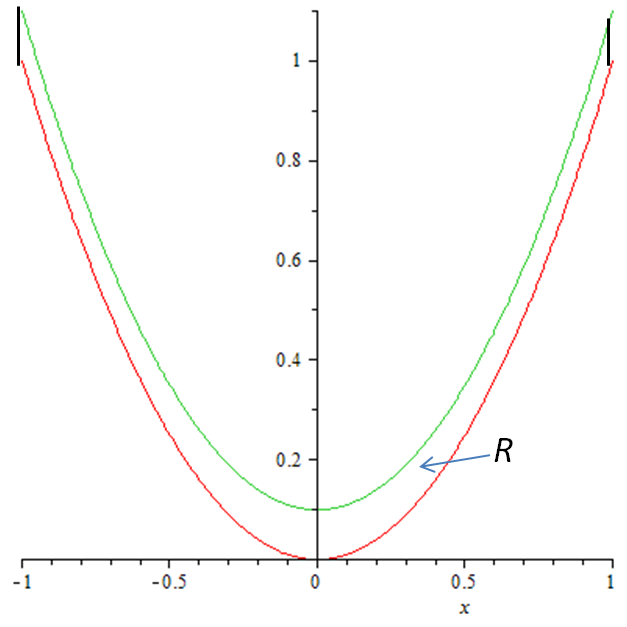
\includegraphics[height=10.58cm,width=10.58cm]{M2S1 Uncorrelated but Dependent.png}\label{figure uncorrelated, dependent}
\caption{The support of $(X,Y)$, where $X \sim Unif(-1,+1)$, $Z \sim Unif(0,0.1)$ and $Y = X^2 + Z$}
\end{center}
\end{figure}

\subsection{Multivariate Transformations}$\;$

\begin{thm}[The Convolution Theorem]$\quad$\par\vspace{1cm}

\noindent\textbf{1: } Let $X$, $Y$ be discrete r.v.s with joint mass function $f_{X,Y}(x,y)$. Define $Z=X+Y$. Then:
$$f_Z(z) = \sum\limits_{\overline{\mathcal{X}}} f_{X,Y}(x,z-x)$$

\noindent\textbf{2: } Let $X$, $Y$ be continuous r.v.s with joint density function $f_{X,Y}(x,y)$. Define $Z=X+Y$ as before. Then:
$$f_Z(z) = \int\limits_{\overline{\mathcal{X}}}\!\! f_{X,Y}(x,z-x)\;\diff x$$

\noindent where, in both the discrete and continuous cases, $\overline{\mathcal{X}}\subseteq\mathcal{X}$ is the set of values that $X$ can take such that $Y$ can take the value $X-z$.

\end{thm}

\noindent\textsc{Proof:}\par\vspace{1cm}
\indent Trivial. Partition the event $\{X+Y=z\}$ into events $\{X=x\}\cap\{Y=z-x\}$, then apply the theorem of total probability.\par\vspace{1cm}

For more general transformations, suppose $(X,Y)$ is a bivariate r.v. and let $U=g_1(X,Y)$, $V=g_2(X,Y)$. Then, for any $B \subseteq \mathbb{R}$:
$$P((U,V)\in B) = P((X,Y) \in A)\; : \; A =\{(X,Y)\; | \; (g_1(X,Y),g_2(X,Y)) \in B\}$$

\noindent If $(X,Y)$ is discrete:
\begin{align*}
f_{U,V}(u,v) &= P((U,V)=(u,v))\\
&= P((X,Y)\in A)\\
&= \!\!\!\!\!\!\!\sum\limits_{(X,Y)\in A} \!\!\!\!\!\!\!\!f_{X,Y}(x,y)
\end{align*}

If $(X,Y)$ is continuous, suppose $g_1$ and $g_2$ are injective. Then we can define $h_1,\; h_2$ s.t. $X=h_1(U,V)$, $Y=h_2(U,V)$. Recall that, in the univariate case:
$$f_U(u) = f_X\left(g^{-1}(u)\right) \left| \frac{\diff}{\diff u}\left(g^{-1}(u)\right)\right|$$
Now, in the bivariate case:
$$f_{U,V}(u,v) = f_{X,Y}(x,y)|J|$$
where $J$ is the \uline{jacobian of the transformation}:
\begingroup
\renewcommand*{\arraystretch}{1.5}
$$J = \left|\begin{array}{cc} \frac{\partial h_1}{\partial u}\quad & \frac{\partial h_1}{\partial v}\\ \frac{\partial h_2}{\partial u}\quad & \frac{\partial h_2}{\partial v}\end{array}\right|$$
\endgroup

Note that the jacobian is itself the determinant of a matrix and so $|J|$ is the \emph{absolute value} of the determinant. Thus, and given the definitions of $h_1$ and $h_2$, we have:

$$|J| = \left| \frac{\partial x}{\partial u}\frac{\partial y}{\partial v} - \frac{\partial y}{\partial u}\frac{\partial x}{\partial v}\right|$$

\begin{ex}
\vspace{1cm}

Let $X \sim \Gamma(r,1),\; Y \sim \Gamma(s,1)$ independent. Define $Z_1=X+Y,\; Z_2=X/(X+Y)$. Find the distribution of $(Z_1,Z_2)$ and the marginals of $Z_1$ and $Z_2$.
\end{ex}

\noindent First we note that, from the independence of $X$ and $Y$ and the definitions of $Z_1$ and $Z_2$,
$$0<Z_1<\infty\qquad\qquad 0<Z_2<1$$

Now, $Z_1 = X/Z_2$, hence $X = Z_1Z_2$, whence $Y=Z_1 - X = Z_1-Z_1Z_2$. Therefore:
\begingroup
\renewcommand*{\arraystretch}{1.5}
\begin{align*}
J &= \left|\begin{array}{cc} \frac{\partial x}{\partial z_1}\quad & \frac{\partial x}{\partial z_2}\\ \frac{\partial y}{\partial z_1}\quad & \frac{\partial y}{\partial z_2}\end{array}\right|\\
&= \left| \begin{array}{cc} z_2 \; & z_1\\ 1-z_2\; & -z_1 \end{array}\right|\\
&= -z_1z_2 - (1-z_2)z_1\\
&= -z_1\\
\Rightarrow\quad |J| &= |z_1|\\
&=z_1
\end{align*}
\endgroup

\noindent By independence,
\begin{align*}
f_{X,Y}(x,y) &= f_X(x)f_Y(y)\\
&= \frac{1}{\Gamma(r)\Gamma(s)}x^{r-1}y^{s-1}e^{-(x+y)}\\
\Rightarrow\quad f_{Z_1,Z_2}(z_1,z_2) &= \frac{1}{\Gamma(r)\Gamma(s)}(z_1z_2)^{r-1}[z_1(1-z_2)]^{s-1}e^{-z_1}z_1\\
&= \frac{1}{\Gamma(r)\Gamma(s)}z_1^{(r-1)+(s-1)+1}z_2^{r-1}(1-z_2)^{s-1}e^{-z_1}\\
&= \frac{1}{\Gamma(r)\Gamma(s)} (z_1^{r+s-1}e^{-z_1}) (z_2^{r-1}(1-z_2)^{s-1})\\
\end{align*}

We see that the joint density function factorises and the supports are independent of one another, so $Z_1$ and $Z_2$ are independent. By examining the \uline{kernel of the distribution}, that is, the part of the density function \emph{dependent on the r.v.} without the normalising constant in front, we can see that $Z_1 \sim Gamma(r+s,1)$ and $Z_2 \sim Beta(r,s)$:
$$f_{Z_1}(z) = \frac{1}{\Gamma(r+s)}z^{r-1}e^{-z}\qquad\qquad f_{Z_2}(z) = \frac{\Gamma(r+s)}{\Gamma(r)\Gamma(s)}z^{r-1}(1-z)^{s-1}$$
\hfill$Q.E.I.$

\subsection{Moments of Sums of Random Variables}\label{moments of sums}$\;$

\begin{defn}[Mean and Variance-Covariance Matrix of a Random Vector]\vspace{1cm}

We can conveniently represent sums (and, more generally, weighted sums) of r.v.s using vector notation.
Let $\vec{X} = (X_1,\; X_2,\; ...\; X_n)^T$ be a \uline{vector-valued} r.v. - that is, a random vector, so that each of its entries, $X_i$ are themselves random variables. Then the mean of $\vec{X}$ is:
$$\vec{\mu_X} = \left(\begin{array}{c}\overline{X_1}\\ \overline{X_2}\\ \vdots\\ \overline{X_n} \end{array}\right)$$
and the \uline{variance-covariance matrix} of $\vec{X}$ is:
$$\Sigma = \left( \begin{array}{cccc} Var(X_1)\quad& Cov(X_1,X_2)\quad& \hdots\quad& Cov(X_1,X_n)\\Cov(X_1,X_2)\quad& Var(X_2)\quad& \hdots\quad& Cov(X_2,X_n)\\ \vdots\quad& \vdots & \vdots\quad & \vdots\\ Cov(X_1,X_n) & Cov(X_2,X_n)\quad& \hdots& Var(X_n) \end{array}\right)$$
that is, the matrix whose i-j element is the covariance of $X_i$ and $X_j$ - noting that the covariance of $X_i$ with itself is simply the variance.

\end{defn}


$\quad$Let $\vec{X}$ be a random $n$-vector with mean $\vec{\mu_X}$ and variance-covariance matrix $\Sigma$. Let $\vec{b}$ be a constant vector, $a$ a scalar constant. Then:
$$E(a+\vec{b}^T\vec{X}) = a + \vec{b}^T\vec{\mu_X}$$
and
$$Var(a + \vec{b}^T\vec{X}) = \vec{b}^T\Sigma\vec{b}$$

The proof is omitted for brevity. It proceeds by simple, direct calculation.


\subsection{Multivariate Generalisations of Univariate Distributions}$\;$

$\quad$In this section we will study 3 multivariate distributions that generalise univariate distributions we have previously encountered.

\subsubsection{The Multinomial Distribution: $\vec{X}\sim Multinomial(n, \vec{p})$}

$\quad$Recall the binomial distribution, which models $n$ independent trials, each with two outcomes, which occur with the same probability in each trial. Now suppose a similar setup, but with $k$ possible outcomes to each trial, each with a fixed probability $p_i$. Let $X_i$ be the number of trials in which outcome $i$ occurred and let the vector of $X_i$ be $\vec{X}$. Then $\vec{X}$ is multinomial and:
$$f_{\vec{X}}(\vec{x}) = \left(\begin{array}{ccccc} & & n\;& & \\ x_1\;&x_2\;&\hdots\;&x_{k-1}\;&x_k\end{array}\right)\prod_{i=1}^k p_i^{x_i}$$
where:
$$\left(\begin{array}{ccccc} & & n\;& & \\ x_1\;&x_2\;&\hdots\;&x_{k-1}\;&x_k\end{array}\right) = \frac{n!}{\prod\limits_{i=1}^k x_i!}$$

The binomial distribution is the special case of the multinomial distribution when $k=2$.

\subsubsection{The Dirichlet Distribution: $\vec{X}\sim Dirichlet(\vec{\alpha})$}

$\quad$The Dirichlet distribution generalises the Beta distribution to multivariate r.v.s. It has p.d.f.:
$$f_{\vec{X}}(\vec{x}) = \frac{\Gamma(\sum\limits_{i=1}^k \alpha_i)}{\prod\limits_{i=1}^k \Gamma(\alpha_i)} \prod_{i=1}^k x_i^{\alpha_i -1}$$

with:
$$0 < x_i < 1\qquad\qquad \sum_{i=1}^k x_i = 1$$

The Beta distribution is the special case for $k=2$.

\subsubsection{The Multivariate Normal Distribution: $\vec{X} \sim MVN(\vec{\mu},\Sigma)$}

$\quad$Let $\vec{X}$ be a vector of Normal r.v.s with mean $\vec{\mu}$ and variance-covariance matrix $\Sigma$. Then $\vec{X}$ is multivariate Normal and:
$$f_{\vec{X}}(\vec{x}) = \frac{1}{\sqrt{2 \pi |\Sigma|}}e^{-\frac{1}{2}(\vec{x}-\vec{\mu})^T\Sigma^{-1}(\vec{x}-\vec{\mu})}$$

\clearpage
\section{Order Statistics}\label{order stats}$\;$

\begin{defn}[Order Statistics]\vspace{1cm}

Suppose we wish to find the distribution of the maximum, minimum or median of a random sample. Given a random sample $X_1,\; X_2,\; ...\; X_n$ i.i.d., we define the \uline{order statistics} $X_{(i)}$ of that sample to be the sample values put in ascending order. That is:
$$\{X_{(1)},\; X_{(2)},\; ...\; X_{(n)}\} = \{X_1,\; X_2,\; ...\; X_n\} \text{ where } X_{(1)}<X_{(2)}< ... < X_{(n)}$$
\end{defn}

Note that here we have assumed that $X_i \neq X_j \; \forall i \neq j$. For continuous distributions, the probability of any individual point is actually 0, so this assumption is reasonable. For discrete distributions, it is not a reasonable assumption. However, we will not consider this issue here. For the purposes of this course, we will assume that all elements of the sample are distinct.

Now, we can clearly see that $X_{(1)}$ is the minimum of the sample, $X_{(n)}$ the maximum and, given $n$ odd, $X_{((n+1)/2)}$ is the median. We can now study the distributions of these statistics. In fact, should we wish too, we can study the distribution of any of the order statistics. For instance, we might be interested in the distributions of the upper and lower quartiles of the data, which are the $[n/4]^{th}$ and $[3n/4]^{th}$ order statistics.

Suppose $X_1,\; ...\; X_n$ i.i.d. are a sample taken from a distribution with c.d.f. $F_X$. Let $Y$ be the $r^{th}$ order statistic: $Y=X_{(r)}$. Then:
\begin{align*}
F_Y(y) &= P(Y\leq y)\\
&= P(\{\text{at least r of the $X_i$ are} \leq y\})
\end{align*}
Note:
$$P(X_i \leq y) = F_X(y)\; \forall i$$

As $X_i$ are i.i.d., the conditions for a binomial process are met, so the number of order statistics less than or equal to $y$ follows a binomial distribution: $(no. \leq y) \sim Binomial(n, F_X(y))$.
$$\Rightarrow \quad F_Y(y) = \sum_{j=r}^n \left(\!\!\!\begin{array}{c} n\\j\end{array}\!\!\!\right) [F_X(y)]^j [1-F_X(y)]^{n-j}$$

Note that although the presence of a sum makes this look like a discrete c.d.f., the sum is \textbf{not} over $\mathcal{Y}$. This is, in fact, generally a continuous distribution.

\clearpage
\section{Hierarchical and Mixture Models}$\;$

By the definition of conditional mass/density fucntions, we can write:
$$f_{X,Y,Z}(x,y,z) = f_{X|Y,Z}(x|y,z) f_{Y|Z}(y|z) f_Z(z)$$
and similar expressions for larger numbers of r.v.s. This allows us to combine models to derive a variety of ``multi-level'' models. This is best illustrated by example:

\begin{ex}[Sizes of Fish]$\quad$\par\vspace{1cm}

Suppose we wish to model the sizes of fish of a particular species in a lake. The Normal distribution is normally a good model for sizes of animals, with a slight catch. Most animals, including fish, mate seasonally. Therefore, there will be a subpopulation of fish conceived in the most recent mating cycle, whose ages will all be very close and whose sizes we expect to follow a Normal distribution with a particular mean and variance, another subpopulation one year older, whose sizes will be Normally distributed \emph{with a different mean and variance}, and so on, the number of subpopulations being equal to the maximum number of years one of these fish can live. Because of this segregation of the population into discrete subpopulations with different size distributions, a Normal model for the whole population will not be accurate. Note that this problem is present to a lesser extent in humans because although, as a species, we mate all year round, the difference in size of the two sexes prevents a Normal model from fitting the whole population appropriately.

Let $X$ denote the size of a fish, $A$ its age (taking $A=1$ for the youngest subpopulation, $A=2$ for the next youngest, \&c.). Then $A$ is a discrete r.v. with support $\mathcal{A} = \{1,2,\; ...\; k\}$, where $k$ is the maximum age of the fish. Let $f_A(a) = \beta_a$, where $\beta_a$ is the ratio of the number of fish of age $a$ to the total number.

Now, we assume a Normal model for size \emph{given that the fish is of a particular age}. That is:
$$f_{X|A}(x|a) \sim N(\mu_a,\sigma_a^2)$$
where $\mu_a$ and $\sigma_a^2$ are, of course, the mean and variance of the size of the fish of age $a$. Then:
\begin{align*}
f_{X,A}(x,a) &= f_{X|A}(x|a) \times f_A(a)\\
&= \beta_a \frac{1}{\sqrt{2 \pi \sigma^2_a}} e^{-(x-\mu_a)^2/2\sigma^2_a}\\
&= \frac{\beta_a}{\sigma_{a}} \phi\left(\frac{x-\mu_a}{\sigma_a}\right)
\end{align*}
where $\phi(x)$ is the standard Normal density function.

But we might not be able to easily measure the age of a given fish directly, so we are more interested in the marginal distribution of $X$:
\begin{align*}
f_X(x) &= \sum_{a=1}^k f_{X,A}(x,a)\\
&= \sum_{a=1}^k \frac{\beta_a}{\sigma_a} \phi\left(\frac{x-\mu_a}{\sigma_a}\right)
\end{align*}
This is effectively a weighted average of Normal distributions. This is an example of a (finite) mixture model.

We can also, of course, derive $f_{A|X}(a|x)$, should we so desire.

\end{ex}

Generally, \uline{mixture models} like the above model populations consisting of a mixture of subpopulations, each of which follows its own distribution for a particular r.v. They are a particular case of \uline{hierarchical models}, which model r.v.s whose parameters are themselves r.v.s (this is extremely useful for modelling uncertainty or measurement error in parameters).

\begin{thm}[Calculating Moments in Hierarchical Models]\label{iterated expectation}\vspace{1cm}

\noindent\textbf{1: } $E_{X}(X) = E_{Y}[E_{{X|Y}}(X|Y)]$

\noindent\textbf{2: } $Var_{X}(X) = E_{Y}[Var_{{X|Y}}(X|Y)] + Var_{Y}[E_{{X|Y}}(X|Y)]$

\end{thm}

\noindent\textsc{Proof:}\par\vspace{1cm}

\textbf{1: }
\begin{align*}
E_{X}(X) &= \int\limits_{\mathcal{X}}\!\! xf_X(x)\;\diff x\\
&= \iint\limits_{\mathcal{X}\times\mathcal{Y}}\!\! xf_{X,Y}(x,y)\;\diff x \diff y\\
&= \iint\limits_{\mathcal{X}\times\mathcal{Y}}\!\! xf_{X|Y}(x|y) f_Y(y)\; \diff x \diff y\\
&= \iint\limits_{\mathcal{X}\times\mathcal{Y}}\!\! xf_{X|Y}(x|y)\;\diff x\; f_Y(y)\; \diff y\\
&= \int\limits_{\mathcal{Y}}\!\! E_{{X|Y}}(X|Y) f_Y(y)\; \diff y\\
&= E_{Y}[E_{X|Y}(X|Y)]
\end{align*} \hfill$\blacksquare$

\textbf{2: }
\begin{align*}
Var_{X}(X) &= E_{{X}}(X^2) - [E_{X}(X)]^2\\
&= \int\limits_{\mathcal{X}}\!\! x^2 f_X(x)\;\diff x - \left[\;\int\limits_{\mathcal{X}}\!\! x f_X(x)\;\diff x\right]^2\\
&= \iint\limits_{\mathcal{X}\times\mathcal{Y}}\!\! x^2 f_{X,Y}(x,y)\;\diff x \diff y - \left[ \;\;\iint\limits_{\mathcal{X}\times\mathcal{Y}}\!\! x f_{X,Y}(x,y)\;\diff x\diff y\right]^2\\
&= \iint\limits_{\mathcal{X}\times\mathcal{Y}}\!\! x^2 f_{X|Y}(x|y) f_Y(y) \;\diff x\diff y - \left[\;\;\iint\limits_{\mathcal{X}\times\mathcal{Y}}\!\! x f_{X|Y}(x|y) f_Y(y) \;\diff x\diff y\right]^2\\
&= \iint\limits_{\mathcal{X}\times\mathcal{Y}}\!\! x^2 f_{X|Y}(x|y) \;\diff x\; f_Y(y)\;\diff y - \left[\;\;\iint\limits_{\mathcal{X}\times\mathcal{Y}}\!\! x f_{X|Y}(x|y)\;\diff x\; f_Y(y)\;\diff y\right]^2\\
&= \int\limits_{\mathcal{Y}}\!\! E_{{X|Y}}(X^2|Y) f_Y(y)\;\diff y - \left[\;\int\limits_{\mathcal{Y}}\!\! E_{{X|Y}}(X|Y) f_Y(y)\;\diff y\right]^2\\
&= E_{Y}[E_{{X|Y}}(X^2|Y)] - (E_{Y}[E_{{X|Y}}(X|Y)])^2\\
&= E_{Y}[Var_{{X|Y}}(X|Y) + (E_{{X|Y}}[X|Y])^2] + Var_{Y}[E_{{X|Y}}(X|Y)] - E_{Y}([E_{{X|Y}}(X|Y)]^2)\\
&= E_{Y}[Var_{{X|Y}}(X|Y)] + E_{Y}([E_{{X|Y}}(X|Y)]^2) + Var_{Y}[E_{{X|Y}}(X|Y)] - E_{Y}([E_{{X|Y}}(X|Y)]^2)\\
&= E_{Y}[Var_{{X|Y}}(X|Y)] + Var_{Y}[E_{{X|Y}}(X|Y)]
\end{align*}\hfill$Q.E.D.$

Note that all the lines with the integrals in the second part could have been omitted by using \textbf{1}. They are included to illustrate that the iterated expectation formula \textbf{1} need not ever be used - it is always possible to solve problems from the definition of expectation - but that to do so can easily double the length of working.

\begin{ex}[Normal-Normal Hierarchical Models]$\quad$\par\vspace{1cm}

Suppose $Y|(\mu,\xi) \sim N(\mu,\sigma^2\xi)$ and $\mu \sim N(\alpha,\tau^2)$, $\xi \sim \chi^2_\nu$, with $\vec{\theta} = (\sigma^2, \alpha, \tau^2, \nu)$ known. Then:
\begin{align*}
E_Y(Y) &= E_{\mu,\xi}[E_{Y|(\mu,\xi)}(Y|(\mu,\xi))]\\
&= E_{(\mu,\xi)}(\mu)\\
&= \alpha\\
Var_Y(Y) &= E_{(\mu,\xi)}[Var_{Y|(\mu,\xi)}(Y|(\mu,\xi))] + Var_{(\mu,\xi)}[E_{Y|(\mu,\xi)}(Y|(\mu,\xi))]\\
&= E_{(\mu,\xi)}(\sigma^2\xi) + Var_{(\mu,\xi)}(\mu)\\
&= \sigma^2E_{(\mu,\xi)}(\xi) + \tau^2\\
&= \sigma^2\nu + \tau^2
\end{align*}

This is much easier than finding the moments by integrating, as we would normally need to do.

\end{ex}

\clearpage
\section{Statistics and their Sampling Distributions}$\;$

\begin{defn}[Simple Random Samples]\vspace{1cm}

A \uline{simple random sample} (or \uline{s.r.s.}) is a number of i.i.d. r.v.s from a given distribution:\\ $X_1,\;X_2,\; ...\; X_n \overset{\text{i.i.d.}}{\sim} f_X(x)$.
\end{defn}

\begin{defn}[Statistics and Sampling Distributions]\vspace{1cm}

A \uline{statistic} is any real-valued function of a s.r.s. A statistic may not involve the parameters of the distribution from which the sample is drawn, but may involve the size of the sample and its values. As a statistic is a function of r.v.s, it is itself a r.v. It's distribution is called the \uline{sampling distribution} for the statistic.

\end{defn}

\begin{ex}[2 Common Statistics]\vspace{1cm}

\noindent\textbf{The sample mean:}
$$\overline{X} = \frac{1}{n} \sum_{i=1}^n X_i$$

\noindent\textbf{The sample variance:}
$$S^2 = \frac{1}{n-1}\sum_{i=1}^n (X_i - \overline{X})^2$$
From the sample variance we can define the sample standard deviation, $S=\sqrt{S^2}$.

\end{ex}

\begin{prop}[Properties of Sample Mean and Variance]\label{sample moments}\vspace{1cm}

Let $X_1,\;\hdots\; X_n$ be a s.r.s. from a distribution with mean $\mu$ and variance $\sigma^2$. Then:

\textbf{1: }
$$(n-1)S^2 = \sum_{i=1}^n X_i^2 - n\overline{X}^2$$

\textbf{2:}
$$E(\overline{X}) = \mu$$

\textbf{3:}
$$Var(\overline{X}) = \frac{\sigma^2}{n}$$

\textbf{4:}
$$E(S^2) = \sigma^2$$

\end{prop}

\noindent\textsc{Proof:}\par\vspace{1cm}

\textbf{1: }
\begin{align*}
(n-1)S^2 &= \sum_{i=1}^n (X_i-\overline{X})^2\\
&= \sum_{i=1}^n X_i^2 - \sum_{i=1}^n \overline{X}^2\\
&= \sum_{i=1}^n X_i^2 - n\overline{X}^2
\end{align*}\hfill$\blacksquare$

\textbf{2:}
\begin{align*}
E(\overline{X}) &= E(\frac{1}{n}\sum_{i=1}^n X_i)\\
&= \frac{1}{n}\sum_{i=1}^n E(X_i)\\
&= \frac{1}{n} \sum_{i=1}^n \mu\\
&= \mu
\end{align*}\hfill$\blacksquare$

\textbf{3:} Let $\vec{X} = (X_1,\; \hdots\; X_n)^T,\; \vec{1} = (1,1,\; \hdots\; 1)^T,\; \Sigma$ the variance-covariance matrix of $\vec{X}$. Then:
\begin{align*}
\Sigma &= \left(\begin{array}{ccc} Var(X_1)\quad& \hdots\quad& Cov(X_1,X_n)\\ \vdots\quad & \ddots\quad & \vdots\\ Cov(X_n,X_1)\quad& \hdots\quad& Var(X_n)\end{array}\right)\\
&= \left(\begin{array}{ccc} \sigma^2\quad& \hdots\quad& 0\\ \vdots\quad & \ddots\quad & \vdots\\ 0\quad &\hdots\quad &\sigma^2\end{array}\right)\quad\mbox{as $X_i$ are i.i.d.}\\
Var(\overline{X}) &= Var(\frac{1}{n}\sum_{i=1}^n X_i)\\
&= \frac{1}{n^2}Var(\vec{1} \cdot \vec{X})\\
&= \frac{1}{n^2} \vec{1}^T\Sigma\vec{1}\quad\mbox{by section \ref{moments of sums}}\\
&= \frac{1}{n^2}n\sigma^2\\
&= \frac{\sigma^2}{n}
\end{align*}\hfill$\blacksquare$

\textbf{4:}
\begin{align*}
E(S^2) &= E\left[\frac{1}{n-1}\left(\sum_{i=1}^n X_i^2 -n\overline{X}^2\right)\right]\quad\mbox{by \textbf{1}}\\
&= \frac{1}{n-1}\left[\sum_{i=1}^n E(X_i^2) - nE(\overline{X}^2)\right]\\
&= \frac{1}{n-1}\left[n(\sigma^2 + \mu^2) - n\left(\frac{\sigma^2}{n} + \mu^2\right)\right]\quad\mbox{by \textbf{2} and \textbf{3}}\\
&= \frac{1}{n-1}(n\sigma^2 + n\mu^2 - \sigma^2 -n\mu^2)\\
&= \sigma^2
\end{align*}\hfill$Q.E.D.$

\subsection{Parameter Estimation}$\;$

\begin{defn}[Estimators and Estimates]\vspace{1cm}

An \uline{estimator} of a parameter is a statistic used to estimate that parameter. As it is a statistic, it is a random variable. An \uline{estimate} is a value taken by an estimator.

\end{defn}

$\overline{X}$ is an estimator of the mean $\mu$ and $S^2$ an estimator of the variance $\sigma^2$. Estimates of these quantities would be the mean, $\overline{x}$, and variance, $s^2$, of a \emph{particular} random sample.

\begin{defn}[The Bias of an Estimator]\vspace{1cm}

Let there be a s.r.s. drawn from a distribution with some unknown parameter $\theta$. Let $T$ be an estimator of $\theta$. Then the \uline{bias} of $T$ is defined to be $E(T) - \theta$. If $E(T) = \theta$, we say that $T$ is an \uline{unbiased} estimator.

\end{defn}

From proposition \ref{sample moments}, we see that $\overline{X}$ and $S^2$ are unbiased estimators of mean and variance respectively. Generally, an unbiased estimator is to be preferred to a biased one, but there are times when an estimator, though biased, might be preferable to an unbiased alternative for some other reason. For instance, if $T$ is an unbiased estimator of $\theta$ with some variance $\sigma_T^2$ and $S$ is a biased estimator with variance $\sigma_S^2\ll \sigma^"_T$, then $S$ might be preferable to $T$ as an estimator if its bias is sufficiently small, as $T$, by virtue of its large variance, might give a value far away from the true value of $\theta$, whereas $S$, though biased, is at least likely to give a value \emph{close to} the true value, even if it is less likely to give the true value exactly. Bias, then, is not the only factor to consider in an estimator.

\subsubsection{The Method of Moments}

$\quad$Suppose we have a s.r.s. $X_1,\;\hdots\; X_n$ from a distribution with unknown parameters $\theta_1,\;\hdots\; \theta_k$, which we wish to estimate. Suppose also we can find an expression for the first $k$ (non-central) moments of the distribution in terms of the $\theta_i$. Then we define the following estimators of these moments:

\begin{align*}
\frac{1}{n}\sum_{i=1}^n X_i &\approx E(X)\\
&\vdots\\
\frac{1}{n}\sum_{i=1}^n X_i^k &\approx E(X^k)
\end{align*}

As the expectations on the right-hand side can be expressed in terms of the $\theta_i$ and the statistics on the left-hand side are all readily calculable from the sample, we have $k$ equations in $k$ unknowns, so we can generally solve for all of the $\theta_i$. This will let us express each of the $\theta_i$ as a function of the above statistics, thus giving us an estimator for each $\theta_i$. This technique is called the \uline{Method of Moments} (M.o.M.).

\begin{ex}[The Method of Moments]\vspace{1cm}

Let $X_i \overset{\text{i.i.d.}}{\sim} Binomial(k,p)$ be a s.r.s., $i = 1,\;\hdots\;n$. Our two M.o.M. equations are:
$$\overline{X}=\frac{1}{n}\sum_{i=1}^n X_i = kp \quad\mbox{ and }\quad \frac{1}{n}\sum_{i=1}^n X_i^2 = kp(1-p) + k^2p^2$$

\begin{alignat*}{3}
\Rightarrow\quad & & \frac{1}{n} \sum_{i=1}^n X_i^2 &= \overline{X} - \overline{X}p + \overline{X}^2\\
& & &= \overline{X} - \frac{\overline{X}^2}{k} + \overline{X}^2\\
\Rightarrow \quad & & \frac{-\overline{X}^2}{k} &= \frac{1}{n}\sum_{i=1}^n X_i^2 - \overline{X}^2 - \overline{X}\\
\Rightarrow\quad & & k &= \frac{\overline{X}^2}{\overline{X}+\overline{X}^2 - \frac{1}{n}\sum\limits_{i=1}^n X_i^2}\\
& & &= \frac{\overline{X}^2}{\overline{X} - \frac{1}{n}\sum\limits_{i=1}^n \left[(X_i - \overline{X})^2\right]}\\
\Rightarrow\quad &  & p &= \frac{\overline{X}}{k}\\
& & &= \frac{\overline{X} - \frac{1}{n}\sum\limits_{i=1}^n \left[(X_i - \overline{X})^2\right]}{\overline{X}}
\end{alignat*}

\end{ex}

The main advantage of the Method of Moments estimates is that they are relatively quick and easy to compute, making them useful for ``back-of-the-envelope'' calculations, or for obtaining an initial estimate for an iterative estimating technique. However, it is not always very accurate (note that the estimators used for all moments but the first are biased) and does not respect parameter spaces - occasionally it can give an impossible value for a parameter, such as a negative estimate for a parameter that is constrained to be positive.

\subsubsection{Maximum Likelihood Estimation}

$\quad$Our objective in parameter estimation is to obtain the ``best'' estimate for unknown parameters. Consider what we mean by ``best.'' If we wish to find the mean height of adult humans, say, and draw a s.r.s. of people, getting heights of 1.78m, 1.56m and 1.63m, it is clearly absurd to postulate a value for the population mean of 2m. This is obvious, but, if you think about it, the \emph{reason} this is such a bad estimate is that if the population mean really were 2m, the probability of obtaining the sample we did would be very low. On the other hand, if the population mean were around 1.66m (the sample mean), then the probability of getting the sample we did would be relatively high. In this way, we can sensibly define the ``best'' estimate of a parameter given a sample to be the value that maximises the probability of obtaining the given sample.

A piece of notation: in the following we speak of the $argmax$ of a function. This is simply the value of the argument which globally maximises the function (of course, this need not be a unique value, or even well-defined). For instance, $argmax_x (1-x^2) = 0$, as the maximum of the function $1 - x^2$ occurs at $x=0$. Similarly, we may, of course, consider the $argmin$. Simply, $argmax_x[f(x)] = a$ where $f(a) = max\{f(x)\}$.

\begin{defn}[The Likelihood Function]\vspace{1cm}

Given a s.r.s. $\vec{X} = (X_1,\; \hdots\; X_n)$ drawn from a distribution with unknown parameters \\$\vec{\theta}=(\theta_1,\;\hdots\; \theta_k)$, the \uline{likelihood} of $\theta$ given the sample is the function:

$$\mathcal{L}(\vec{\theta} | \vec{X}) = P(\vec{X} | \vec{\theta})$$

\noindent By the independence of a s.r.s., we can factorise the likelihood function as:

$$\mathcal{L}(\vec{\theta} | \vec{X}) = \prod_{i=1}^n P(X_i | \vec{\theta})$$

Note that, although the function is written as a function of $\vec{\theta}$ conditional upon $\vec{X}$, it is in fact the opposite - a function of $\vec{X}$ conditional upon $\vec{\theta}$. This notation reflects a shift in emphasis, not in the actual direction of the conditioning. We are interested in the probability of a given value for the parameter given a sample and are using as a proxy for this the probability of the sample given values of the parameters, as described above.

As the likelihood function consists of a product of many terms, it is often convenient to take its logarithm (usually to the natural base) and thus convert the product into a sum. We thus define the \uline{loglikelihood} function:

\begin{align*}
l(\vec{\theta} | \vec{X}) &=\log[\mathcal{L}(x)]\\
&= \sum_{i=1}^n \log\left[P\left(X_i | \vec{\theta}\right)\right]
\end{align*}

\end{defn}

\begin{defn}[Maximum Likelihood Estimation]\vspace{1cm}

Given a s.r.s., the \uline{maximum likelihood estimate} (\uline{m.l.e.}), $\hat{\theta}$, of a parameter $\theta$ of the sampling distribution is the value that maximises the probability of drawing the sample that was, in fact, obtained:

$$\hat{\theta} = argmax_\theta \left[\mathcal{L}\left(\vec{\theta} | \vec{X}\right)\right]$$

As the logarithm function is strictly monotone, its stationary points occur at the same values and with the same characters (i.e., maximum, minimum or inflected point) as the stationary points of its argument. Thus we can also express the m.l.e. of $\theta$ as:

$$\hat{\theta} = argmax_\theta \left[l\left(\vec{\theta} | \vec{X}\right)\right]$$

Of course, when attempting to maximise this, we will typically differentiate; sums are much easier to differentiate than products, so this is why the loglikelihood function is far more convenient than the simple likelihood.

\end{defn}

This, then, gives us a method for estimating a parameter from a sample. We express the probability of getting the given sample given a value of the parameter as if it were instead a function of the parameter given the sample values, then find the value of the parameter which maximises this probability (usually by considering its logarithm). In a certain sense, this value can be considered the ``best'' estimate for the parameter, as it is the one which makes the sample we have maximally likely. Its downfall comes when the sample is unlikely under \emph{any} reasonable value for the parameter; but, by definition, this happens but rarely.

\begin{ex}[Maximum Likelihood Estimation for a Continuous Parameter Space]\vspace{1cm}

Let $X_i \overset{\text{i.i.d.}}{\sim} N(\mu, \sigma^2)$ for $i = 1,\;\hdots\; n$ be a s.r.s. We wish to estimate $\vec{\theta} = (\mu,\sigma^2)$.

\begin{align*}
\mathcal{L}(\vec{\theta}|\vec{X}) &= \prod_{i=1}^n \frac{1}{\sqrt{2 \pi \sigma^2}} e^{\frac{-(x_i - \mu)^2}{2\sigma^2}}\\
&= (2\pi\sigma^2)^{-n/2} e^{\frac{-1}{2\sigma^2} \sum\limits_{i=1}^n (x_i - \mu)^2}\\
\Rightarrow \quad l(\vec{\theta}|\vec{X}) &= -\frac{n}{2}\log(2\pi) - \frac{n}{2}\log(\sigma^2) - \frac{1}{2\sigma^2} \sum_{i=1}^n (x_i - \mu)^2\\
\Rightarrow\quad \frac{\partial l}{\partial \mu} &= \frac{1}{\sigma^2}\sum_{i=1}^n(x_i - \mu)\\
\frac{\partial l}{\partial \sigma^2} &= \frac{-n}{2\sigma^2} + \frac{1}{2\sigma^4}\sum_{i=1}^n(x_i - \mu)^2
\end{align*}

\noindent Setting both partial derivatives equal to zero to find the stationary points:
\begin{align*}
\frac{\partial l}{\partial \mu} = 0 \quad&\Leftrightarrow\quad \sum_{i=1}^n x_i - \sum_{i=1}^n \mu = 0 & \frac{\partial l}{\partial \sigma^2} = 0 \quad&\Leftrightarrow\quad \frac{-n}{2\sigma^2} + \frac{1}{2\sigma^4}\sum_{i=1}^n (x_i - \mu)^2 = 0\\
&\Rightarrow\quad \hat{\mu} = \bar{X} & &\Rightarrow\quad \hat{\sigma}^2 = \frac{1}{n} \sum_{i=1}^n (X_i - \bar{X})^2
\end{align*}

We must now confirm that this stationary point is indeed a maximum. This may be done by considering second partial derivatives and is omitted for brevity.

\end{ex}

When the parameter can take any value in a continuous range, as above, we typically maximise by differentiating and setting the derivative equal to zero; when the parameter's values are constrained to a finite or countable set, some more subtle methods are required. It is often convenient to consider the \uline{forward difference operator} (see M1M2), which acts like a discrete analogue of the derivative, or a \uline{forward} \uline{quotient operator}, which can be more tractable in maximum likelihood problems because of cancellations. This is best illustrated by example.

\begin{defn}[The Forward Difference and Quotient Operators]\vspace{1cm}

Given any ordered (finite or countable) sequence of values $a_n$, the \uline{forward difference operator} $\Delta$ is defined by:
$$\Delta(n) = a_{n+1}-a_n$$

Similarly, the \uline{forward quotient operator} (or forward ratio operator) $R$ is defined by:
$$R(n) = \frac{a_{n+1}}{a_n}$$

\end{defn}

These two operators can, like the differential operator, give us information about the rate of change of a function. If $\Delta(n) < 0$, the sequence is decreasing at the $n^{th}$ term; if $\Delta(n) > 0$, the sequence is increasing at the $n^{th}$ term. If $\Delta(n) = 0$, then $a_n = a_{n+1}$ and the sequence can be viewed as having a stationary point at the $n^{th}$ term. The same results hold for $R(n)$, but with 1 substituted for 0.

\begin{ex}[Maximum Likelihood Estimation for a Countable Parameter Space]\vspace{1cm}

Let $X_i \overset{\text{i.i.d.}}{\sim} Binomial(k,p)$, with $p$ known, $k$ unknown (this is highly unrealistic, but we will make this assumption for illustrative purposes). $k \in \mathbb{Z}_+$, so differentiating w.r.t. $k$ is not a permissible approach, in general. Of course, it might be that the maximum found by differentiating will occur at an integer value, in which case the problem is solved, but generally this will not be the case. First, we find the likelihood function:

$$\mathcal{L}(k | \vec{X},p) = \prod_{i=1}^n \frac{k!}{x_i! (k - x_i)!} p^{x_i} (1-p)^{k-x_i}$$

Now, the $x_i$ are to be regarded as known values (when we have a sample, we know the values found in the sample), so this is a function purely of $k$, which is constrained to positive integer values, so we can consider the sequence $\mathcal{L}(k | \vec{X},p)$ and define the forward quotient operator on this sequence:

\begin{align*}
R(k) &= \frac{\mathcal{L}(k+1 | \vec{X},p)}{\mathcal{L}(k | \vec{X},p)}\\
&= \frac{\prod\limits_{i=1}^n \frac{(k+1)!}{x_i! (k+1-x_i)!} p^{x_i} (1-p)^{k+1-x_i}}{\prod\limits_{i=1}^n \frac{k!}{x_i!(k-x_i)!} p^{x_i}(1-p)^{k-x_i}}\\
&= \frac{[(k+1)(1-p)]^n}{\prod\limits_{i=1}^n (k+1-x_i)}
\end{align*}

If the forward quotient is equal to 1, then consecutive terms in the sequence are equal, which is necessary and sufficient for the forward difference to be 0, which is equivalent to the derivative being 0, so we wish to find the value(s) of $k$ such that the forward ratio is 1. Of course, as $k$ is constrained to integer values, this might never occur, so we seek the value for which the forward ratio comes as close to unity as we can achieve. For convenience, we henceforth consider $R(k-1)$.

\begin{align*}
R(k-1) = 1 \quad&\Leftrightarrow\quad [k(1-p)]^n = \prod_{i=1}^n (k-x_i)\\
&\Leftrightarrow\quad k^n(1-p)^n = k^n \prod_{i=1}^n \left(1 - \frac{x_i}{k}\right)\\
&\Leftrightarrow\quad (1-p)^n = \prod_{i=1}^n (1-zx_i)\quad \textrm{where } z = \frac{1}{k}
\end{align*}

Now, we note that $k$ has no upper bound, but is certainly positive, so $z>0$. Also, $k \geq max\{x_i\}$, as there clearly cannot be fewer trials than there are successes in a binomial process. Hence $z \leq max\{x_i\}$. This gives us constraints for $z$: $0<z\leq 1/max\{x_i\}$

Note that as $z \rightarrow 0$, the right-hand side of the above expression tends to unity. The right-hand side is equal to 0 when $z = 1/max\{x_i\}$. Within the range $(0,1]$, the right-hand side is decreasing in $z$. This allows us to sketch a graph of $\prod_{i=1}^n (1-zx_i)$ against $z$ (figure \ref{figure discrete MLE}).

\begin{figure}[h]
\begin{center}
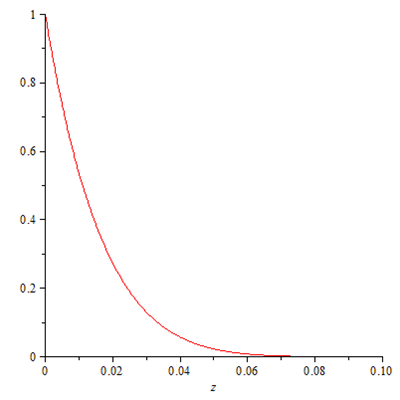
\includegraphics[height=7cm,width=7cm]{M2S1 Discrete MLE.png}\label{figure discrete MLE}
\caption{$\prod\limits_{i=1}^n (1-zx_i)$ for $z$ from 0 to $1/max\{x_i\}$}
\end{center}
\end{figure}

We can see from the sketch that the function plotted is decreasing in the range of interest, so we can expect a unique solution to $(1-p)^n = \prod_{i=1}^n (1-zx_i)$, which was the necessary and sufficient condition for the forward quotient to be unity, which occurs at the maximum of the likelihood. So we solve this equation for $z$ (perhaps by numerical methods), and then take the reciprocal, which is the value of $k$ such that $R(k-1) = 1$. Of course, this might not be an integer value, but we should expect that the maximum should occur at either of the integers adjacent to this value. So we then manually check the comparative sizes of the likelihood at these two values and the largest is therefore the maximum likelihood. The value of $k$ for which this occurs is thus the m.l.e. of $k$.

\end{ex}



Sometimes, we might not have the complete data available to calculate the expectation. This is often the case for continuous distributions due to measurement errors; it can also arise due to participant non-responsiveness in surveys. We therefore use the expectation of the data and iteratively approach an estimate. This is best illustrated by example.

\begin{ex}[The Expectation-Maximisation Algorithm]\vspace{1cm}

Let $X_i \overset{\text{i.i.d.}}{\sim} N(\mu, 1)$ be a s.r.s. Due to measurement errors (rounding), we observe $\{(a_i,b_i)\}\; : \; a_i < X_i < b_i$. With the complete data, maximum likelihood estimation would be easy:

\begin{align*}
\mathcal{L}\left(\mu \big| \vec{X}\right) &= \prod_{i=1}^n \frac{1}{\sqrt{2\pi}} \exp\left[\frac{-(x_i-\mu)^2}{2}\right]\\
\Rightarrow\quad l\left(\mu \big| \vec{X}\right) &= \frac{-n}{2} \log(2\pi) - \frac{1}{2} \sum_{i=1}^n (x_i - \mu)^2\\
&= \mu \sum_{i=1}^n x_i - \frac{n \mu^2}{2} + c
\end{align*}

Note that we have subsumed the terms constant in $x_i$ into a constant $c$; this is because these terms do not affect the location of the maximum (they will disappear upon differentiation) and so their actual values are irrelevant.

Letting $X_{obs}$ denote the observed data and $\mu_0$ an initial estimate of the mean (perhaps a M.o.M. estimate), the expected loglikelihood of $\mu$ given $\vec{X}$ conditional upon $X_{obs}$ is:

\begin{align*}
E\left[l\left(\mu | \vec{X}\right) \bigg| \; X_{obs},\mu_0\right] &= E\left(\mu \sum_{i=1}^n X_i - \frac{n\mu^2}{2} + c\;\Bigg|\; X_{obs},\mu_0\right)\\
&= \mu_0 \sum_{i=1}^n E(X_i \mid X_{obs}) - \frac{n\mu_0^2}{2} + c
\end{align*}

So we need to find $E(X_i \mid a_i < X_i < b_i)$.

Let $Z \sim N(0,1)$ such that $Z=X-\mu$. Then:
$$E(X\mid a<X<b) = E(Z \mid a-\mu<Z<b-\mu) + \mu$$

We therefore have the problem of finding the expectation of a Normal r.v. given that it is between two limits. Define a r.v. $Y$ to have the following density:
$$f_Y(y) = \left\{ \begin{array}{cl} k\phi(y)\quad& : u<y<v\\ 0 \quad& \mbox{otherwise}\end{array}\right.$$
where $\phi(z)$ is the standard Normal density function and $u,v$ are constants. Then, as the p.d.f. of any r.v. must enclose unit area:
\begin{align*}
\int_u^v\!\! f_Y(y)\;\diff y = 1 \quad &\Leftrightarrow\quad \int_u^v \!\! \phi(z) \diff z = \frac{1}{k}\\
&\Leftrightarrow\quad k = \frac{1}{\Phi(v) - \Phi(u)}
\end{align*}
Whence we conclude:
\begin{align*}
E(Z \mid u<Z<v) &= E(Y)\\
&= \int_u^v \!\! \frac{y\phi(y)}{\Phi(v)-\Phi(u)}\;\diff y\\
&= \frac{\int_u^v \!\! \frac{y}{\sqrt{2\pi}} e^{-y^2/2}\;\diff y}{\Phi(v)-\Phi(u)}\\
&= \frac{\left[\frac{-1}{\sqrt{2\pi}}e^{-y^2/2}\right]_u^v}{\Phi(v)-\Phi(u)}\\
&= \frac{\phi(u)-\phi(v)}{\Phi(v)-\Phi(u)}
\end{align*}\hfill$Q.E.I.$

\noindent Hence:
$$E(X_i \mid a_i< X_i<b_i) = \frac{\phi(a_i-\mu_0)-\phi(b_i-\mu_0)}{\Phi(b_i-\mu_0)-\Phi(a_i-\mu_0)}+\mu_0$$
Denote this quantity by $X_i^{(1)}$. Then:

\begin{align*}
E\left[l\left(\mu | \vec{X}\right) \bigg| \; X_{obs},\mu_0\right] &= \mu_0 \sum_{i=1}^n X_i^{(1)} - \frac{n\mu_0^2}{2} + c\\
\Rightarrow\quad \frac{\partial E(l)}{\partial \mu} &= \sum_{i=1}^n X_i^{(1)} - n\mu_0\\
&= 0 \quad\Leftrightarrow\quad \mu = \frac{1}{n}\sum_{i=1}^n X_i^{(1)}
\end{align*}

So we let our revised estimate of $\mu$ be:
$$\mu_1 = \frac{1}{n} \sum_{i=1}^n \frac{\phi(a_i-\mu_0)-\phi(b_i-\mu_0)}{\Phi(b_i-\mu_0)-\Phi(a_i-\mu_0)}+\mu_0$$

We can then use this revised estimate to obtain $X_i^{(2)}$, the expected loglikelihood given the observed (incomplete) data and $\mu_1$, whence we can find $\mu_2$. Iterating in this manner, we can converge to an estimate for $\mu$ \hfill$Q.E.F.$

\end{ex}

\subsubsection{Bayesian Inference}

\begin{defn}[Prior and Posterior Distributions]\vspace{1cm}

The \uline{prior distribution}, $f_\Theta(\theta)$ summarises our state of knowledge/belief about a parameter $\theta$ before we observe the data (from a sample). The \uline{posterior distribution} $f_{\Theta \mid X}(\theta \mid x)$ summarises our revised state of knowledge after observing the data.

\end{defn}

By Bayes' theorem:
$$f_{\Theta \mid X}(\theta\mid x) = \frac{f_{X\mid\Theta}(x\mid \theta) \times f_{\Theta}(\theta)}{f_X(x)}$$

We can use the \uline{posterior mean}, $E_{\Theta|X}(\Theta | X)$ as an estimator of the mean and the posterior variance to model uncertainty in the estimate. We can then formulate a distribution for the r.v. explicitly in terms of the parameters for $\Theta$. Bayesian inference requires formulating a prior distribution for the unknown parameter(s). Cf. example \ref{envelope}.

There is an important difference in philosophy between Bayesian inference and the two methods of parameter estimation covered above (M.o.M. and M.L.E.). In the two previous methods, the parameter to be estimated is regarded as an unknown constant. In Bayesian parameter estimation, it is instead treated as if it itself were a random variable. By using the uncertainty in the value of the parameter to model the parameter as a r.v., we can apply the techniques of probability, but this requires us to specify a prior distribution for the parameter, which can be problematic, and to use the more general, subjective interpretation of probability.

\begin{ex}[Bayesian Inference in a Binomial Distribution]\vspace{1cm}

Suppose $Y\mid\Theta \sim Binomial(n,\theta)$, where $n$ is known and we have a prior distribution for $\theta$: $\Theta \sim Beta(\alpha,\beta)$ (the Beta distribution is often useful for modelling probabilities, as its support is the interval $(0,1)$). $\alpha$ and $\beta$ are referred to as \uline{hyperparameters}. Given $\alpha$ and $\beta$, find the marginal distribution of $Y$ and its mean and variance.

The joint distribution of $Y$ and $\Theta$ is given by:

\begin{align*}
f_{Y,\Theta}(y,\theta) &= f_\Theta(\theta) \times f_{Y\mid\Theta}(y\mid\theta)\\
&= \left(\begin{array}{c} \!\!n\!\! \\ \!\!y\!\!\end{array}\right)\theta^y (1-\theta)^{n-y} \times \frac{\Gamma(\alpha + \beta)}{\Gamma(\alpha)\Gamma(\beta)}\theta^{\alpha-1} (1-\theta)^{\beta -1}\\
&= \left(\begin{array}{c}\!\!n\!\! \\ \!\!y\!\!\end{array}\right) \frac{\Gamma(\alpha + \beta)}{\Gamma(\alpha)\Gamma(\beta)} \theta^{y+\alpha-1} (1-\theta)^{n+\beta - y -1}
\end{align*}

We are now in a position to calculate the posterior distribution of $\Theta$ given our datum $Y$. Note that denominator in the Bayes' theorem expression for the prior distribution is dependent only on $Y$; as we are conditioning on $Y$, this can be treated as a constant. This allows us to write a proportionality instead of equality and neglect the prior distribution of $Y$, which would require further calculation. We can then manipulate the kernel of the distribution until we recognise it as a distribution, then simply affix the appropriate normalising constant. This technique works because we know that the result must be a valid p.d.f. (or p.m.f.), so we can proceed back from a proportionality to an equality. This simplifies the calculations hugely in many problems.

\begin{align*}
f_{\Theta\mid Y}(\theta\mid y) &\propto f_{Y,\Theta}(y,\theta)\\
&\propto \theta^{y+\alpha-1} (1-\theta)^{n+\beta-y-1}
\end{align*}
which is recognisably the kernel of a Beta distribution, so we conclude: $\Theta\mid Y \sim Beta(y+\alpha,n+\beta-y)$. Hence:
$$f_{\Theta\mid Y}(\theta\mid y) = \frac{\Gamma(\alpha+\beta+n)}{\Gamma(y+\alpha)\Gamma(n+\beta -y)} \theta^{y+\alpha-1} (1-\theta)^{n+\beta-y-1}$$

We can now find the marginal distribution of $Y$ in terms of the hyperparameters. For convenience, define the Beta function:

$$B(\alpha,\beta) = \frac{\Gamma(\alpha)\Gamma(\beta)}{\Gamma(\alpha + \beta)}$$

\begin{align*}
f_Y(y) &= \frac{f_{\Theta,y}(\theta,y)}{f_{\Theta\mid Y}(\theta \mid y)}\\
&= \frac{\left(\!\!\begin{array}{c} n\\y \end{array}\!\!\right) \frac{1}{B(\alpha,\beta)} \theta^{y+\alpha-1} (1-\theta)^{n-y+\beta-1}}{\frac{1}{B(y+\alpha,n-y+\beta)} \theta^{y+\alpha-1} (1-\theta)^{n-y+\beta -1}}\\
&= \left(\!\!\begin{array}{c} n\\y \end{array}\!\!\right) \frac{B(y+\alpha,n-y+\beta)}{B(\alpha,\beta)}\\
&= \frac{B(y+\alpha,n-y+\beta)}{B(y+1,n-y+1)B(\alpha,\beta)}
\end{align*}

By theorem \ref{iterated expectation} and the standard results for the Beta and Binomial distributions:

\begin{align*}
E_Y(Y) &= E_\Theta[E_{Y\mid \Theta}(Y\mid\Theta)]\\
&= E_\Theta(n\Theta)\\
&= \frac{n\alpha}{\alpha+\beta}
\end{align*}
\begin{center} and \end{center}
\begin{align*}
Var_Y(Y) &= E_\Theta[Var_{Y\mid\Theta}(Y\mid\Theta)] + Var_\Theta[E_{Y\mid\Theta}(Y\mid\Theta)]\\
&= E_\Theta[n\Theta(1-\Theta)] + Var_\Theta(n\Theta)\\
&= nE_\Theta(\Theta) - n[E_\Theta(\Theta)]^2 + n^2 Var_\Theta(\Theta)\\
&=  \frac{n\alpha\beta(\alpha+\beta+n)}{(\alpha+\beta)^2(\alpha+\beta+1)}
\end{align*}\hfill$Q.E.I.$

\end{ex}

Note that, in the above example, the prior and posterior distributions of $\Theta$ are the same distribution, simply with different parameters. This is a particular relationship between the Binomial distribution (of $Y$) and the Beta distribution; we say that the Beta distribution is the \uline{conjugate prior} of the Binomial. For this reason, the marginal distribution of $Y$ is called a ``Beta-Binomial distribution.''

In the special case where $\alpha = \beta = 1$, the Beta distribution is the same as the standard Uniform distribution, so $\Theta \sim Unif(0,1)$, which models absolute uncertainty about $\theta$, allowing it to take any value in its permitted range with equal probability. In this case, the mean and variance of the marginal distribution of $Y$ are found to be:

$$E_Y(Y) = \frac{n}{2} \qquad Var_Y(Y) = \frac{n}{12}(n+2)$$

\begin{defn}[Conjugate Prior Distributions]\vspace{1cm}

If the prior and posterior distributions of a parameter of a particular sampling distribution are of the same family, we say that the prior distribution is the \uline{conjugate prior} to that sampling distribution.

\end{defn}

\subsection{Confidence Intervals}$\;$

Let $X \sim N(\mu,\sigma^2)$. Consider the interval $\mathscr{J}(X) = (X-1.96\sigma,X+1.96\sigma)$, which is an \emph{interval-valued} random variable, or \uline{random interval}. Recall that, for a Normal r.v., $95\%$ of the data lie within $1.96\sigma$ of the mean:
$$P(\mu-1.96\sigma < X < \mu+1.96\sigma) = 95\%$$

We are interested in when the interval $\mathscr{J}(X)$ contains $\mu$. Define $\mathcal{I}=\mathscr{J}(\mu) = (\mu-1.96\sigma,\mu+1.96\sigma)$. Then, clearly:

\begin{align*}
&\mu \in \mathscr{J}(X) \quad \Leftrightarrow\quad X \in \mathcal{I}\\
\Rightarrow\quad &P[\mu\in \mathscr{J}(X)] = 95\%
\end{align*}

95\% of the intervals thus calculated will therefore contain $\mu$. This gives us a measure, then, of our certainty of the value of $\mu$. If the interval is wide, there is a large range of values which $\mu$ could take; conversely, a small interval means we know $\mu$ very precisely. Such an interval is called a \uline{95\% confidence interval}. Other sizes of interval are, of course, possible, but 95\% is the accepted standard; it is called the \uline{confidence level}. It is common practice in scientific papers to give results with a 95\% confidence interval; for instance, a value obtained in an experiment might be reported as ``$12.4 \pm 0.9$'' or ``$7.3\; {}^{+2.1}\!\!/\!\!{}_{-0.3}$,'' say (note that the interval need not be centred around the estimate). When it is not specifically stated what confidence level is used, 95\% may be assumed.

We use confidence intervals (C.I.s) to show our certainty of estimates of parameters including, but not limited to, the mean.

It is important to note that confidence intervals are \emph{not} generally unique. When multiple intervals contain the same probability mass (95\% or whatever the confidence level is), the shortest is usually given by preference, as it more precisely specifies the estimate. Fig \ref{confidence intervals} illustrates this.

\begin{figure}[h]
\begin{center}
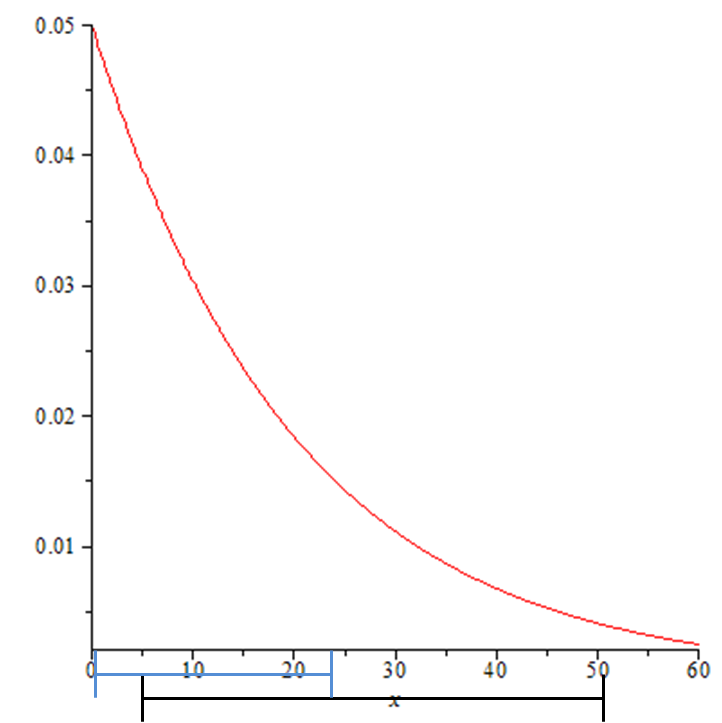
\includegraphics[height=10cm,width=10cm]{M2S1 Confidence Intervals.png}\label{confidence intervals}
\caption{An exponential density function with two 70\% confidence intervals; the shortest (in blue) and a longer C.I. (black). The blue C.I. would be preferred.}
\end{center}
\end{figure}

\subsubsection{Bayesian Intervals}$\;$

Suppose we have used Bayesian inference to derive the posterior distribution of a parameter, $\theta$, given a datum $X$ (or several data, $\vec{X}$). Then we can compute a $(1-\alpha)\times 100\%$ central interval:
$$\left[ F_{\Theta\mid X}^{-1} \left(\frac{\alpha}{2}\right), F_{\Theta\mid X}^{-1} \left(1-\frac{\alpha}{2}\right)\right]$$
where $\alpha \in (0,1)$. For instance, we would use $\alpha=0.95$ for a 95\% interval.

Such an interval has a probability $\alpha$ of containing the 'true' value of $\theta$; note, however, that it might not be the shortest such interval, so it is not necessarily optimal.

There is an important philosophical difference between frequentist C.I.s and Bayesian intervals. A confidence interval is a \emph{random interval} and 95\% (say) of sampled values of this interval will contain the parameter, which is an unknown but \emph{fixed constant}. A Bayesian interval models the \emph{parameter itself} as a r.v., as there is uncertainty in its value, and creates a \emph{fixed, constant interval} such that there is a 95\% chance that the parameter will lie therein. It is important to remember that the randomness is in our \emph{estimate}, not inherent in the parameter itself.

\subsubsection{Pivots}$\;$

Suppose we have a s.r.s. from a Normal distribution with known variance but unknown mean, for which we wish to derive a confidence interval: $X_i \sim_{i.i.d.} N(\mu,\sigma^2)$. Then we can show by the convolution theorem that $\bar{X} \sim N(\mu,\sigma^2/n)$. Therefore, by a location-scale transformation:
$$\frac{\bar{X}-\mu}{\sigma/\sqrt{n}}\sim N(0,1)$$

\begin{alignat*}{3}
&\Rightarrow\quad P\left(-1.96 \leq \frac{\bar{X}-\mu}{\sigma/\sqrt{n}} \leq +1.96\right) &= 95\%\\
&\Rightarrow\quad P\left(-1.96\frac{\sigma}{\sqrt{n}} -\bar{X} \leq -\mu \leq +1.96\frac{\sigma}{\sqrt{n}} - \bar{X}\right) &= 95\%\\
&\Rightarrow\quad P\left(\bar{X}-1.96\frac{\sigma}{\sqrt{n}} \leq \mu \leq \bar{X} +1.96\frac{\sigma}{\sqrt{n}}\right) &= 95\%\\
&\Rightarrow\quad \left(\bar{X}-1.96\frac{\sigma}{\sqrt{n}}\; ,\;\bar{X}+1.96\frac{\sigma}{\sqrt{n}}\right) \mbox{ is a 95\% C.I. for $\mu$} & &
\end{alignat*}

Clearly, this method can easily be adapted for computing intervals at confidence levels other than 95\%. This is an example of a useful general method for finding C.I.

The quantity $(\bar{X}-\mu)\sqrt{n}/\sigma$ used above has a known distribution and is in terms of known quantities ($\bar{X}$ and $\sigma$) and the parameter $\mu$ for which we seek a C.I. Such a quantity is called a \emph{pivot}.\par\vspace{1cm}

\begin{defn}[Pivots]\vspace{1cm}

A \uline{pivot} is a function of a random sample, known population parameters, and precisely one unknown parameter, for which it is desired to find a C.I., which has a known distribution.

\end{defn}

\begin{ex}[Using Pivots when Multiple Parameters are Unknown]\vspace{1cm}

Suppose $X_i \overset{\text{i.i.d.}}{\sim} N(\mu,\sigma^2)$, as before, except that this time, we know neither $\mu$ nor $\sigma^2$. Again, suppose we seek a C.I. for $\mu$.

The quantity:
$$\frac{\bar{X}-\mu}{\sigma/\sqrt{n}} \sim N(0,1)$$

is no longer a pivot, as $\sigma$ is now also unknown. However, the quantity:
$$\frac{(n-1)S^2}{\sigma^2} \sim \chi^2_{n-1}$$

is a pivot for $\sigma$, so we can solve for this and hence obtain a pivot for $\mu$:
\begin{align*}
\text{let } T &= \frac{\frac{\bar{X}-\mu}{\sigma/\sqrt{n}}}{\sqrt{S^2/\sigma^2}}\\
&= \frac{\bar{X}-\mu}{S/\sqrt{n}}
\end{align*}

Recall:
$$Z\sim N(0,1) \quad \wedge\quad U \sim \chi^2_\nu \quad \Rightarrow\quad \frac{Z}{\sqrt{U/\nu}} \sim t_\nu$$

$$\Rightarrow\quad T \sim t_{n-1}$$

So $T$ is a function of $\mu$ and known values only and follows a known distribution. Hence $T$ is a pivot for $\mu$ and can be used to find a C.I.

\end{ex}

\subsection{Jensen's Inequality and Bias}$\;$

\begin{defn}[Convex and Concave Functions]\vspace{1cm}

A function $f$ is said to be \uline{convex} on an interval $I$ if:
$$\forall x\in I\;f''(x) \geq 0$$\par\vspace{1cm}

Conversely $f$ is said to be \uline{concave} on $I$ if:
$$\forall x \in I \; f''(x) \leq 0$$\par\vspace{1cm}

\end{defn}

\begin{thm}[Jensen's Inequalities]\vspace{1cm}

\textbf{1: } if $g$ is a convex function on the support of $X$, then:
$$E_X[g(X)] \geq g[E_X(X)]$$\par\vspace{1cm}

\textbf{2: } if $g$ is concave on the support of $X$, then:
$$E_X[g(X)] \leq g[E_X(X)]$$\par\vspace{1cm}

In both cases, equality holds iff $P[g(X) = a+bX] = 1$ for some $a$ and $b$; i.e., if $g$ is linear on the support of $X$.

\end{thm}

\noindent\textsc{Graphical Proof:}\par\vspace{1cm}

\begin{figure}[h]
\begin{center}
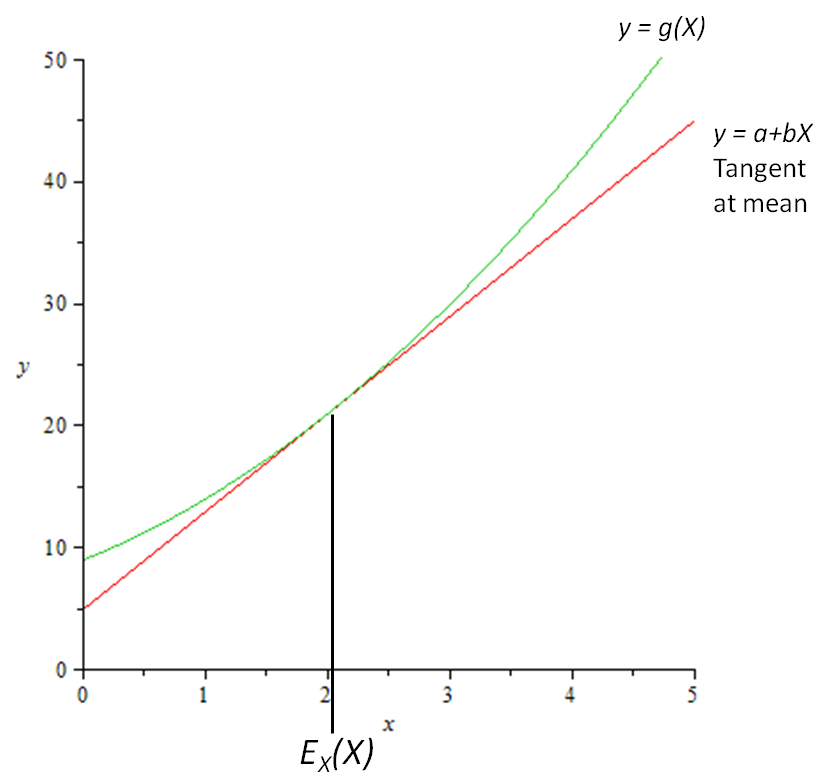
\includegraphics[height=12.86cm,width=13.8cm]{M2S1 Jensen's Inequalities.png}\label{jensen}
\caption{A convex function of $X$ and the tangent to that function at the mean.}
\end{center}
\end{figure}

As $g$ is convex, $g(X)\geq a+bX\;\forall X$. Hence:
\begin{align*}
E_X[g(X)] &\geq E_X(a+bX)\\
&=a+bE_X(X)\\
&= g[E_X(X)]
\end{align*}\hfill$Q.E.D.$

And similarly for $g$ concave.

\begin{ex}

Let $X\sim Binomial(n,p)$. Define $\hat{p} = X/n$ is an estimator of $p$.
\begin{align*}
E_X(\hat{p}) &= \frac{1}{n}E_X(X)\\
&= \frac{1}{n}np\\
&= p
\end{align*}

so $\hat{p}$ is an unbiased estimator of $p$.

Suppose we wish to estimate the odds ratio, $\xi$ (see M1S):
$$\xi = \frac{p}{1-p}=g(p)$$

We find that:
$$g''(p) = 2(1-p)^{-3} >0 \mbox{ on $[0,1]$}$$

so $g$ is convex on the support of $\hat{p}$.

Let $\hat{\xi} = g(\hat{p}) = \hat{p}/(1-\hat{p})$ be an estimator of the odds ratio. Then, by Jensen's inequality (using a strict inequality, as we know $g$ is non-linear):
\begin{align*}
E_X\left(\hat{\xi}\right) &> g[E_X(\hat{p})]\\
&= g(p)\\
&= \frac{p}{1-p}\\
&= \xi
\end{align*}

So we see that $\hat{\xi}$ is an (upwardly) biased estimator - it tends to overestimate the odds ratio. This is despite the fact that it is derived from an unbiased estimator.

\end{ex}

Generally speaking, bias is \emph{not} invariant under transformation. The exception is for linear transformations, which preserve bias, as can be seen from the necessary and sufficient condition for equality in Jensen's inequalities.


\clearpage
\section{Convergence}$\;$

\subsection{Convergence in Distribution}$\;$

\begin{defn}[Convergence in Distribution]\vspace{1cm}

A sequence of r.v.s $X_i$ is said to \uline{converge in distribution} to the r.v. $Y$ if:
$$\lim_{n\to\infty}\left[F_{X_n}(x)\right] = F_Y(x) \;\mbox{$\forall x$ at which $F_Y$ is continuous}$$

We write: $X_n \xrightarrow{\mathscr{D}}Y$

\end{defn}

\begin{defn}[Degeneracy]\vspace{1cm}

If $X_n \xrightarrow{\mathscr{D}} Y$ and $P(Y=c) = 1$ for some constant $c$, s.t.:
$$F_Y(y) = \left\{\begin{array}{cc} 0\quad &:\quad x<c\\ 1\quad&:\quad x\geq c \end{array}\right.$$
then we say that the limiting distribution of $X_n$ is \uline{degenerate} at $c$ and write $X_n \xrightarrow{\mathscr{D}} c$

\end{defn}

\begin{defn}[Moment Generating Functions]\vspace{1cm}

Recall from M1S that the \uline{moment generatign function} (\uline{m.g.f.}) of the r.v. $X$ is:
$$M_X(t) = E_X(e^{tX})$$

provided that this expectation exists in some neighbourhood of zero.

\end{defn}

\begin{thm}[Calculating Moments from M.G.F.s]\vspace{1cm}

Recall from M1S: if $X$ has a m.g.f., then:
\begin{align*}
E_X(X^n) &= M_X^{(n)}(0)\\
&= \left.\frac{\diff^n M_X(t)}{\diff t^n}\right|_{t=0}
\end{align*}

\end{thm}

\noindent\textsc{Sketch Proof:}\par\vspace{1cm}

\begin{align*}
\dot{M}_X(t) &= \frac{\diff}{\diff t}\left(\int\!\! e^{tx}f_X(x)\;\diff x\right)\\
&= \int\!\!\frac{\diff}{\diff t}\left(e^{tx}f_X(x)\right)\;\diff x\\
&= \int\!\!\frac{\diff}{\diff t}\left(e^{tx}\right)f_X(x)\;\diff x\\
&= \int\!\! xe^{tx}f_X(x)\;\diff x\\
&= E_X\left(Xe^{tX}\right)\\
\Rightarrow\quad \dot{M}_X(0) &= E\left(Xe^0\right)\\
&= E(X)
\end{align*}

and similarly for higher moments.

\begin{thm}[Properties of M.G.F.s]\label{mgf properties}\vspace{1cm}

\textbf{1: }
$$M_{aX+b}(t) = e^{bt}M_X(at)$$\par\vspace{1cm}

\textbf{2: } let $X_1,\;\hdots\;X_n$ be a sequence of independent r.v.s with m.g.f.s $M_{X_1}(t),\;\hdots\;M_{X_n}(t)$ respectively.\\ \indent\indent Let $Z= X_1 + \hdots + X_n$. Then:
$$M_Z(t) = \prod_{i=1}^n M_{X_i}(t)$$\par\vspace{1cm}

\textbf{3: } let $(X_1,\;\hdots\;X_n)$ be i.i.d. r.v.s, each with m.g.f. $M_X(t)$. Then:
$$M_{\bar{X}}(t) = \left[M_X\left(\frac{t}{n}\right)\right]^n$$\par\vspace{1cm}

\textbf{4: } if $M_X(t)$ exists (in a neighbourhood of zero), then for $r=0,\;1,\;2,\;\hdots$:\par
\indent\indent \textbf{(I) }  $\;\,M_X^{(r)}(t)$ exists near zero\par
\indent\indent \textbf{(II) }  $E\left(\left|X^r\right|\right) < \infty$\par

\textbf{5 (Characterisation): } if $X$ and $Y$ have m.g.f.s and $M_X(t) = M_Y(t)$ in a neighbourhood of zero,\\ \indent\indent then $F_X(u) = F_Y(u)\;\forall u$. I.e., m.g.f.s are sufficient to characterise distributions.\par\vspace{1cm}

\textbf{6 (Convergence of m.g.f.s): } Let $X_1,\;X_2,\;\hdots$ be a countable sequence of r.v.s with m.g.f.s $M_{X_i}(t)$\\ \indent\indent s.t.:
$$\lim_{i\to\infty}\left[M_{X_i}(t)\right] = M_X(t)$$
\indent\indent for $t$ in a neighbourhood of zero, $M_X(t)$ an m.g.f. Then there is a unique c.d.f. $F_X(x)$ with\\ \indent\indent moments determined by $M_X(t)$ and for which:
$$\lim_{i\to\infty}\left[F_{X_i}(x)\right] = F_X(x)$$
\indent\indent for all $x$ at which $F_X(x)$ is continuous. I.e., $X_n\xrightarrow{\mathscr{D}}X$

\end{thm}

\noindent\textsc{Partial Proof:}\par\vspace{1cm}

\textbf{1: }
\begin{align*}
M_{aX+b}(t) &= E_X\left[e^{(aX+b)t}\right]\\
&= E_X\left[e^{aXt}\right]e^{bt}\\
&= e^{bt}M_X(at)\qquad\square
\end{align*}

\textbf{2: }
\begin{align*}
M_Z(t) &= E_Z\left[e^{\left(X_1+\hdots + X_n\right) t}\right]\\
&= E_Z\left[\prod_{i=1}^n e^{X_i t}\right]\\
&= \prod_{i=1}^n E_{X_i}\left(e^{X_it}\right)\\
&= \prod_{i=1}^n M_{X_i}(t)\qquad\square
\end{align*}

\textbf{3: } follows directly from \textbf{1} and \textbf{2}\par\vspace{1cm}

\textbf{4-6:} beyond the scope of this course. Proof requires the study of Laplace transforms.\par\vspace{1cm}

The above theorem (in particular, part \textbf{6}) allows us to show convergence in distribution by showing convergence of m.g.f.s in a neighbourhood of zero. Although convergence of m.g.f.s is a sufficient condition for convergence in distribution, it is not necessary (after all, the m.g.f. might not even exist). There is a more general strategy, involving \uline{characteristic functions} of the form $\phi_X(t) = E_X\left(e^{itX}\right)$. This is beyond the scope of this course.

Note that moments alone do not characterise distributions. Two r.v.s can have identical moments but not be identically distributed. Identity of m.g.f.s is stronger than identity of all moments. However, if $X$ and $Y$ have \emph{finite support}, then they are identically distributed iff their moments are identical. I.e.,:
$$F_X(u) \equiv F_Y(u)\quad\Leftrightarrow\quad E_X(X^r) \equiv E_Y(Y^r)$$

\subsection{The Central Limit Theorem}$\;$

\begin{thm}[The Central Limit Theorem]\vspace{1cm}

Let $X_1,\;\hdots$ be a sequence of i.i.d. r.v.s, each with m.g.f. $M_X(t)$. Define $\bar{X}_n$ to be the sample mean of the first $n$ $X$'s; i.e.:
$$\bar{X}_n = \frac{1}{n}\sum_{i=1}^n X_i$$

Hence define $G_n(x)$ to be the c.d.f. of $\sqrt{n}(\bar{X}_n -\mu)/\sigma$, where $\mu$ and $\sigma$ are the mean and standard deviation of the distribution of the $X_i$. Then:
\begin{align*}
\lim_{n\to\infty}\left[G_n(x)\right] &= \int_{-\infty}^{x}\!\! \frac{1}{\sqrt{2\pi}}e^{-\frac{y^2}{2}}\;\diff y\\
&= \Phi(x)\\
\text{i.e., } G_n &\xrightarrow{\mathscr{D}} \Phi\\
\text{i.e., } \frac{\sqrt{n}\left(\bar{X}_n -\mu\right)}{\sigma} &\xrightarrow{\mathscr{D}} N(0,1)
\end{align*}

\end{thm}

\noindent\textsc{Proof:}\par\vspace{1cm}

Note: by assumption, $M_X(t)$ exists in some neighbourhood of zero and $\mu$ and $\sigma^2$ exist.

By theorem \ref{mgf properties}, it suffices to prove:
\begin{align*}
\lim_{n\to\infty}\left[M_{\sqrt{n}\left(\bar{X}_n -\mu\right)/\sigma}(t)\right] &= M_Z(t) \mbox{ where $Z\sim N(0,1)$}\\
&= e^{\frac{t^2}{2}}
\end{align*}

Let $W_i =\left(X_i-\mu\right)/\sigma$, s.t.:
$$\frac{\sqrt{n}\left(\bar{X}_n-\mu\right)}{\sigma} = \frac{1}{\sqrt{n}}\sum_{i=1}^n W_i$$

Note:
$$E_{W_i}(W_i) = 0 \qquad Var_{W_i}(W_i) = 1$$

By Taylor's theorem:
\begin{align*}
M_{W_i}(t) &= \sum_{k=0}^s \frac{M_{W_i}^{(k)}(0)t^k}{k!} + \frac{M_{W_i}^{(s+1)}\left(\xi\right)t^{s+1}}{(s+1)!} \mbox{ where $\left|\xi\right|<|t|$}\\
&= M_{W_i}(0) + \dot{M}_{W_i}(0)t + \frac{1}{2}\ddot{M}_{W_i}\left(\xi\right)t^2 \mbox{ for $s=1$}\\
&= E_{W_i}\left(e^0\right) + E_{W_i}\left(W_i\right) + \frac{1}{2}\ddot{M}_{W_i}\left(\xi\right)t^2\\
&= 1 + 0 + \frac{1}{2}\ddot{M}_{W_i}\left(\xi\right)t^2
\end{align*}

Now, from the definition of $W_i$ and theorem \ref{mgf properties}:
\begin{align*}
\lim_{n\to\infty}\left[M_{\sqrt{n}\left(\bar{X}_n-\mu\right)/\sigma}(t)\right] &= \lim_{n\to\infty}\left[M_{\sum\limits_{i=1}^n W_i/\sqrt{n}}(t)\right]\\
&= \lim_{n\to\infty}\left(\left[M_{W_i}\left(\frac{t}{\sqrt{n}}\right)\right]^n\right)\\
&= \lim_{n\to\infty}\left(\left[1+\frac{t^2}{2n}\ddot{M}_{W_i}(s_n)\right]^n\right) \mbox{ where $s_n = \frac{\xi}{\sqrt{n}}: |s_n| < \frac{|t|}{\sqrt{n}}$}\\
&= \exp\left(\lim_{n\to\infty}\left[n\log\left(1 + \frac{t^2}{2n}\ddot{M}_{W_i}(s_n)\right)\right]\right)\\
&= \exp\left(\lim_{n\to\infty}\left[\frac{t^2}{2}\ddot{M}_{W_i}(s_n)\frac{\log\left(1+\frac{t^2}{2n}\ddot{M}_{W_i}(s_n)\right) - \log(1)}{\frac{t^2}{2n}\ddot{M}_{W_i}(s_n)}\right]\right)
\end{align*}

Now, we know, by assumption, that $\dddot{M}_{W_i}$ exists in some neighbourhood of zero, so $\ddot{M}_{W_i}$ is continuous in this region. Hence:
\begin{align*}
\lim_{n\to\infty}\left[\ddot{M}_{W_i}(s_n)\right] &= \ddot{M}_{W_i}\left(\lim_{n\to\infty}[s_n]\right)\\
&= \ddot{M}_{W_i}(0) \mbox{ for $|s_n| < |t|/\sqrt{n}$}\\
&= E_{W_i}\left(W_i^2\right)\\
&= Var_{W_i}\left(W_i\right) + \left[E_{W_i}\left(W_i)\right)\right]^2\\
&= 1
\end{align*}

Therefore:
$$\lim_{n\to\infty}\left[\frac{t^2}{2n}\ddot{M}_{W_i}(s_n)\right] = 0$$

Let:
$$\delta_n = \frac{t^2}{2n}\ddot{M}_{W_i}(s_n)$$

Then $\delta_n \to 0$ as $n\to\infty$. Then:
\begin{align*}
\lim_{n\to\infty}\left[\frac{\log\left(1+\delta_n\right) - \log(1)}{\delta_n}\right] &= \lim_{\epsilon\to 0}\left[\frac{\log\left(1+\epsilon\right)-\log(1)}{\epsilon}\right]\\
&= \left.\frac{\diff \log(x)}{\diff x}\right|_{x=1}\\
&= 1
\end{align*}

Using the above results and basic properties of limits, we conclude:
\begin{align*}
\lim_{n\to\infty}\left[M_{\sqrt{n}\left(\bar{X}_n-\mu\right)/\sigma}(t)\right] &= \exp\left(\frac{t^2}{n}\right)\\
&= M_Z(t)\\
\Rightarrow\quad \frac{\sqrt{n}\left(\bar{X}_n-\mu\right)}{\sigma} &\xrightarrow{\mathscr{D}} N(0,1)
\end{align*}\hfill$Q.E.D.$

Recall section \ref{normal approx to bin}, in which we used the Normal distribution to approximate the Binomial distribution for suitable values of the parameters. We can now see why that is permissible. The Central Limit Theorem (C.L.T.) allows us to approximate the standardised mean from any distribution with a finite mean and variance and an extant m.g.f. by a Normal distribution, in the limit as the sample size goes to infinity.

In fact, the requirement of an m.g.f. is not needed, but the proof in the more general case is prohibitively long and difficult for this course. The C.L.T. may, however, be assumed, even for distributions whose m.g.f. does not exist. Be careful, however, as the requirement of finite mean and variance cannot be relaxed. The Cauchy distribution, for example, does not have finite variance and so it \emph{does not} obey the C.L.T. This next example will show us a partial way around this obstacle.

\begin{ex}\vspace{1cm}

Suppose $X_i \overset{\text{i.i.d.}}{\sim} Unif(0,1)$. Let:
$$M_n = X_{(r)}\; :\; r=\frac{n+1}{2}$$

be the median, with $n$ odd (this is not entirely necessary, but simplifies things). Find the limiting distribution of $M_n$ and $S_n = (M_n - 1/2)n^p$ for a constant $p$.\par\vspace{1cm}

Recall from section \ref{order stats} the c.d.f. of the $r^{th}$ order statistic:
$$F_{M_n}(x) = \sum_{j=r}^n \binom{n}{j}x^j (1-x)^{n-j}$$

which is equal to $P(J\geq r)$ where $J\sim Binomial(n,x)$, so:
\begin{align*}
F_{M_n}(x) &= P(J\geq r)\\
&= P\left(\frac{J-nx}{\sqrt{nx(1-x)}} \geq \frac{r-nx}{\sqrt{nx(1-x)}}\right)\\
&= P\left(\frac{J-nx}{\sqrt{nx(1-x)}} \geq \frac{n+1-2nx}{2\sqrt{nx(1-x)}}\right)
\end{align*}

We know, from the Central Limit Theorem, that a standardised Binomial converges in distribution to a standard Normal. Hence:
$$\frac{J-nx}{\sqrt{nx(1-x)}} \xrightarrow{\mathscr{D}} N(0,1)$$

Also, as $n\to\infty$:
$$\frac{n+1-2nx}{2\sqrt{nx(1-x)}} \rightarrow \left\{\begin{array}{cc} +\infty \quad&:\quad x<1/2\\ 0\quad&:\quad x=1/2\\-\infty\quad&:\quad x>1/2\end{array}\right.$$

Hence, as $n\to\infty$:
\begin{align*}
P(J\geq r) &\to \left\{\begin{array}{cc} P(Z\geq +\infty)\quad&:\quad x<1/2\\ P(Z \geq 0)\quad&:\quad x=1/2\\ P(Z\geq -\infty\quad&:\quad x>1/2\end{array}\right.\\
&= \left\{\begin{array}{cc} 0\quad&:\quad x<1/2\\ 1/2\quad&:\quad x=1/2\\ 1\quad&:\quad x>1/2\end{array}\right.\\
\Rightarrow\quad M_n &\xrightarrow{\mathscr{D}} \frac{1}{2}
\end{align*}\hfill$Q.E.I.$

Now, $S_n = (M_n - 1/2)n^p$:
\begin{align*}
P(S_n\leq s) &= P\left[ \left(M_n-\frac{1}{2}\right)n^p \leq s\right]\\
&= P\left(M_n \leq \frac{1}{2} + sn^{-p}\right)\\
&= \sum_{i=r}^n \binom{n}{i} \left(\frac{1}{2}+sn^{-p}\right)^i\left(\frac{1}{2}-sn^{-p}\right)^{n-i}\\
&= P(I\geq r) \mbox{ where $I\sim Binomial\left(n,\frac{1}{2}+sn^{-p}\right)$}\\
&= P\left(\frac{I-\frac{n}{2}-sn^{1-p}}{\sqrt{n\left(\frac{1}{2} + sn^{-p}\right)\left(\frac{1}{2}-sn^{-p}\right)}} \geq \frac{r-\frac{n}{2}-sn^{1-p}}{\sqrt{n\left(\frac{1}{2} + sn^{-p}\right)\left(\frac{1}{2}-sn^{-p}\right)}}\right)\\
&= P\left(\frac{I-\frac{n}{2}-sn^{1-p}}{\sqrt{n\left(\frac{1}{2} + sn^{-p}\right)\left(\frac{1}{2}-sn^{-p}\right)}} \geq \frac{\frac{n+1}{2}-\frac{n}{2} - sn^{1-p}}{\sqrt{n\left(\frac{1}{2}+sn^{-p}\right)\left(\frac{1}{2}-sn^{-p}\right)}}\right)\\
&=  P\left(\frac{I-\frac{n}{2}-sn^{1-p}}{\sqrt{n\left(\frac{1}{2} + sn^{-p}\right)\left(\frac{1}{2}-sn^{-p}\right)}} \geq \frac{\frac{1}{2}-sn^{1-p}}{\sqrt{\frac{n}{4}-s^2n^{1-2p}}}\right)\mbox{ write the second term as $c_n$:}\\
&= P\left(\frac{I-\frac{n}{2}-sn^{1-p}}{\sqrt{n\left(\frac{1}{2} + sn^{-p}\right)\left(\frac{1}{2}-sn^{-p}\right)}} \geq c_n\right)
\end{align*}

By the Central Limit Theorem, we know that this tends to a Normal probability. If $c_n\to\pm\infty$, we will obtain a degenerate probability; to avoid this, pick $p=1/2$:
\begin{align*}
c_n &= \frac{\frac{1}{2}-s\sqrt{n}}{\sqrt{\frac{n}{4}-s^2}}\\
&= \frac{1}{2\sqrt{\frac{n}{4}-s^2}} - \frac{s}{\sqrt{\frac{1}{4}-\frac{s^2}{n}}} \to -2s \mbox{ as $n\to\infty$}\\
\Rightarrow\quad P(S_n\leq s) &\to 1-\Phi(-2s)\\
&=\Phi(2s)\mbox{ by the symmetry of the Normal distribution}\\
\mbox{so } P(S_n\leq s)&\to P(Z\leq 2s)\mbox{ where $Z\sim N(0,1)$}\\
&= P\left(\frac{Z}{2}\leq s\right)\\
\Rightarrow\quad S_n &\xrightarrow{\mathscr{D}} \frac{Z}{2}\\
\mbox{i.e., } \sqrt{n}\left(M_n - \frac{1}{2}\right) &\xrightarrow{\mathscr{D}} \frac{Z}{2}\\
\Rightarrow\quad 2\sqrt{n}\left(M_n - \frac{1}{2}\right) &\xrightarrow{\mathscr{D}} N(0,1)
\end{align*}\hfill$Q.E.I.$

\end{ex}

This example illustrates an important property of the median; that for a s.r.s. from \emph{any} distribution, the distribution of the standardised median converges to a Normal distribution. So, although the C.L.T. requires the sampling distribution to have a finite mean and variance for the mean to converge to the Normal distribution, the median will converge to Normal for absolutely any distribution, even pathological examples like the Cauchy distribution.

\subsection{Convergence in Probability}$\;$

\begin{defn}[Convergence in Probability]\vspace{1cm}

A sequence $X_1,\;X_2,\;\hdots$ of r.v.s is said to \uline{converge in probability} to the distribution of the r.v. $X$ if:
$$\forall\epsilon>0\;\lim_{n\to\infty} \left[P\left(\left|X_n-X\right|<\epsilon\right)\right] = 1$$

or, equivalently:
$$\forall\epsilon >0\;\lim_{n\to\infty}\left[P\left(\left|X_n-X\right|\geq\epsilon\right)\right] = 0$$

We write $X_n \xrightarrow{\mathscr{P}} X$.

\end{defn}

\begin{thm}[Convergence in Probability and in Distribution]\vspace{1cm}

$$X_n\xrightarrow{\mathscr{P}} X \quad\Rightarrow\quad X_n\xrightarrow{\mathscr{D}} X$$

\end{thm}

\noindent\textsc{Proof (continuous case):}\par\vspace{1cm}

Suppose $X_n \xrightarrow{\mathscr{P}}X$. Now, by the theorem of total probability, for any $t$ and $\forall \epsilon>0$:
$$P(X\leq t-\epsilon) = P(X\leq t-\epsilon \AND \left|X_n-X\right| < \epsilon) + P(X\leq t-\epsilon \AND\left|X_n-X\right| \geq \epsilon)$$

Now note that:
\begin{align*}
(X\leq t-\epsilon \AND \left|X_n-X\right| < \epsilon) &\imply (X\leq t-\epsilon \AND X_n-X<\epsilon)\\
&\imply (X+\epsilon\leq t \AND X_n < X + \epsilon)\\
&\imply X_n\leq t\\
&\imply P(X\leq t-\epsilon)\leq P(X_n\leq t) + P(\left|X_n-X\right|\geq \epsilon)
\end{align*}

By similar reasoning:
$$P(X_n\leq t) \leq P(X\leq t+\epsilon)+P(\left|X_n-X\right|\geq \epsilon)$$

Combining the above two results:
$$P(X\leq t-\epsilon) - P(\left|X_n-X\right|\geq \epsilon) \leq P(X_n\leq t) \leq P(X\leq t+\epsilon)+P(\left|X_n-X\right|\geq \epsilon)$$

Taking $n\to\infty$,
$$P(\left|X_n-X\right|\geq \epsilon)\to 0 \mbox{ by assumption}$$

$$\imply P(X\leq t-\epsilon) \leq \lim_{n\to\infty}\left[P(X_n\leq t)\right] \leq P(X\leq t+\epsilon)$$

Now, as $\epsilon\to 0$, by the sandwich theorem:
\begin{align*}
P(X_n\leq t) &\to P(X\leq t)\\
\text{i.e., } F_{X_n}(t) &\to F_X(t)\\
\text{i.e., } X_n \xrightarrow{\mathscr{D}} X
\end{align*}\hfill$Q.E.D.$\par\vspace{1cm}

Note that the converse is not true. Convergence in distribution generally \emph{does not imply} convergence in probability. However, degenerate convergence in distribution \emph{does} imply convergence in probability:
$$X_n\xrightarrow{\mathscr{D}} c \imply X_n \xrightarrow{\mathscr{P}} c$$

\begin{thm}[Slutsky's Theorem]\vspace{1cm}

If $X_n\xrightarrow{\mathscr{D}} X$ and $Y_n\xrightarrow{\mathscr{D}}c$, then:
$$X_nY_n\xrightarrow{\mathscr{D}} cX \mbox{ and } X_n+Y_n\xrightarrow{\mathscr{D}} X+c$$

\end{thm}

\noindent\textsc{Proof:}\par\vspace{1cm}

Beyond the scope of this course. Result may be assumed.\par\vspace{1cm}

\subsection{The Weak Law of Large Numbers}$\;$

\begin{thm}[Chebyshev's Inequality]\vspace{1cm}

Let $X$ be a r.v. and g(X) a non-negative function thereof. Then:
$$\forall r>0\; P\left[g(X)\geq r\right] \leq \frac{E_X\left[g(X)\right]}{r}$$

\end{thm}

\noindent\textsc{Proof:}\par\vspace{1cm}

\begin{align*}
E_X\left[g(X)\right] &= \int\limits_{\mathcal{X}}\!\! g(x)f_X(x)\;\diff x\\
&\geq \int\limits_{A}\!\! g(x)f_X(x)\;\diff x \mbox{ where $A = \left\{x\in\mathcal{X}\mid g(X) \geq r\right\}$}\\
&\geq \int\limits_{A}\!\! rf_X(x)\;\diff x\\
&= r \int\limits_{A}\!\! f_X(x)\;\diff x\\
&= r P\left(X\in A\right)\\
&= r P\left[g(X)\geq r\right]\\
\imply P\left[g(X)\geq r\right] &\leq \frac{E_X\left[g(X)\right]}{r}
\end{align*}\hfill$Q.E.D.$\par\vspace{1cm}


\begin{defn}[Consistent Estimators]\vspace{1cm}

If $T_n$ is a statistic used to estimate some parameter $\theta$, we say $T_n$ is a \uline{consistent estimator} if $T_n\xrightarrow{\mathscr{P}}\theta$

\end{defn}

\begin{thm}[The Weak Law of Large Numbers (W.L.L.N.)]\vspace{1cm}

Suppose $X_1,\;X_2,\;\hdots \overset{\text{i.i.d.}}{\sim} f_X(x)$ is a sequence of i.i.d. r.v.s with:
$$E_X(X_i) = \mu\quad \text{ and }\quad Var_X(X_i) = \sigma^2 < \infty$$

Let $\bar{X}_n$ be the mean of the first $n$:
$$\bar{X}_n = \frac{1}{n} \sum_{i=1}^n X_i$$

Then $\bar{X}_n\xrightarrow{\mathscr{P}}\mu$. I.e.:
$$\forall \epsilon > 0 \;\lim_{n\to\infty}\left[P\left(\left|\bar{X}_n-\mu\right|<\epsilon\right)\right] = 1$$

That is, the sample mean is a consistent estimator of the population mean.

\end{thm}

\noindent\textsc{Proof:}\par\vspace{1cm}

Let $g(X) = (X-\mu)^2$. This function is non-negative, so Chebyshev's Inequality applies. Fix $\epsilon>0$ and let $r=\epsilon^2$. So $r>0$. Then, by Chebychev's Inequality:
\begin{align*}
P\left[(X-\mu)^2 \geq \epsilon^2\right] &\leq \frac{\sigma^2}{\epsilon^2}\\
\imply P(|X-\mu|\geq \epsilon) &\leq \frac{\sigma^2}{\epsilon^2}
\end{align*}

Now, substitute $\bar{X}_n$ for $X$ and $E_X\left(\bar{X}_n\right)$ for $\mu$:
$$P\left(\left|\bar{X}_n - E_X\left(\bar{X}_n\right)\right|\geq \epsilon\right) \leq \frac{\sigma^2}{n\epsilon^2}$$

as $Var_X\left(\bar{X}_n\right) = \sigma^2/n$. But $E_X\left(\bar{X}_n\right) = \mu$. So:
\begin{align*}
\lim_{n\to\infty}\left[P\left(\left|\bar{X}_n-\mu\right|\geq \epsilon\right)\right] &= 0\\
\imply \lim_{n\to\infty}\left[P\left(\left|\bar{X}_n-\mu\right| < \epsilon\right)\right] &= 1\\
\text{i.e., } \;\bar{X}_n &\xrightarrow{\mathscr{P}} \mu
\end{align*}\hfill$Q.E.D.$


\end{document}
